\documentclass[10pt,letterpaper]{article}

%% -packages-
\usepackage{graphics}
\usepackage{psfrag}
\usepackage[round]{natbib}
\usepackage{longtable}
\usepackage{rotating}
\usepackage{rotate}
\usepackage{lscape}
\usepackage{amssymb}
\usepackage{amsmath}
\usepackage[colorlinks,bookmarks,citecolor=magenta]{hyperref}
\usepackage{color}
\usepackage{multicol}
\usepackage{alltt}


%\usepackage[latin1]{inputenc} % To use characters such as � without typing \'e
%\usepackage[cyr]{aeguill} % To display characters such as �
%\usepackage{xspace} % To get the right spacings in front of : and so on
\usepackage[french,english]{babel}

%% ---------------------------------------------------------------------
%%Page Layout Properties-------------------------------------------------

%\voffset 0in \textwidth 7.0in  \oddsidemargin 0in
%\evensidemargin 0in \headheight 0.in \textheight 9in  %%Look at Box13.1 for text scale
\voffset -0.75in
\hoffset -0.75in
\textwidth 6.5in%
\textheight 9.0in%
%\evensidemargin 0.in%

%\textwidth 6in%
%\topmargin 0in%
\setlength{\LTcapwidth}{\textwidth} %caption width for longtables

%Arial font
\renewcommand{\rmdefault}{ppl} % Arial
\renewcommand{\sfdefault}{ppl} % Arial phv  % palatino ppl

%Logo
\usepackage{fancyhdr}
\renewcommand{\headheight}{0.6in}
\setlength{\headwidth}{\textwidth}
\fancyhead[L]{}% empty left
\fancyhead[R]{ % right
   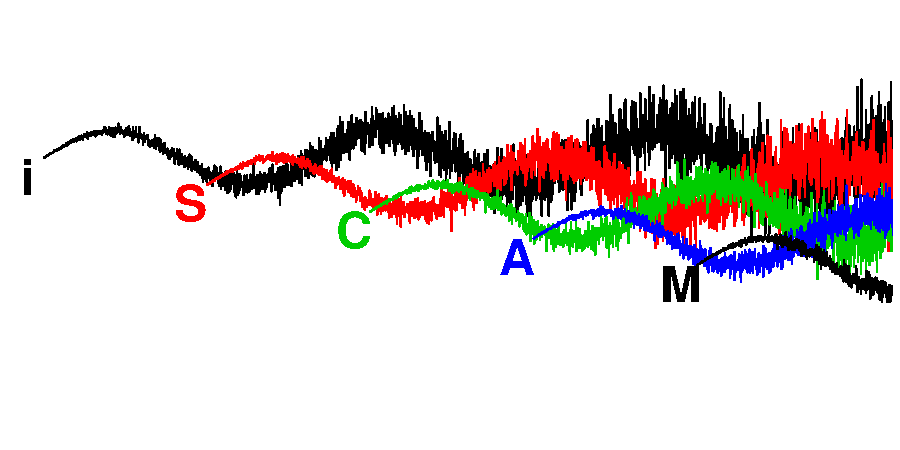
\includegraphics[height=0.53in]{iscamlogo.eps}
}
\pagestyle{fancy}


%-------------------------------------------------------------------------
%Water mark
%%\usepackage{eso-pic}
%%\usepackage{graphicx}
%%\usepackage{color}
%%\usepackage{type1cm}
%%\usepackage{float} 
%%
%%\makeatletter
%%  \AddToShipoutPicture{%
%%    \setlength{\@tempdimb}{.5\paperwidth}%
%%    \setlength{\@tempdimc}{.5\paperheight}%
%%    \setlength{\unitlength}{1pt}%
%%    \put(\strip@pt\@tempdimb,\strip@pt\@tempdimc){%
%%      \makebox(0,0){\rotatebox{45}{\textcolor[gray]{0.85}{\fontsize{1.75cm}{1.75cm}\selectfont{DRAFT  \today}}}}
%%    }
%%} \makeatother


%% -math-
\newcounter{saveEq}
  \def\putEq{\setcounter{saveEq}{\value{equation}}}
  \def\getEq{\setcounter{equation}{\value{saveEq}}}
  \def\tableEq{ % equations in tables
    \putEq \setcounter{equation}{0}
    \renewcommand{\theequation}{T\arabic{table}.\arabic{equation}}
    \vspace{-5mm}
    }
  \def\normalEq{ % renew normal equations
    \getEq
    \renewcommand{\theequation}{\arabic{section}.\arabic{equation}}}

  \def\puthrule{ %thick rule lines for equation tables
    \hrule \hrule \hrule \hrule \hrule}


%%\newcommand{\msy}{$C^*$}
%%\newcommand{\fmsy}{$F^*$}
%%\newcommand{\sbmsy}{$\rm{SB_{MSY}}$}
%%\newcommand{\sbfour}{$\rm{SB_{40}}$}
%%\newcommand{\�}{\'e}
%%\newcommand{\�}{\`e}
%%\newcommand{\�}{\`a}
%%\newcommand{\�}{\^e}
\newcommand{\iscam}{
{$^i$}\textcolor{red}{S}\textcolor{green}{\small{}C}{\textcolor{blue}{\footnotesize{}A}}\textcolor{black}{$_\textnormal{M}$}}%{\raisebox{-0.7ex}{M}}%

\newcommand{\fmsy}{F$_{\textnormal{MSY}}$}
\newcommand{\bmsy}{B$_{\textnormal{MSY}}$}

%% ---------------------------------------------------------------------


\makeatletter
\newenvironment{tablehere}
  {\def\@captype{table}}
  {}

\newenvironment{figurehere}
  {\def\@captype{figure}}
  {}
\makeatother

%% ---------------------------------------------------------------------


\title{
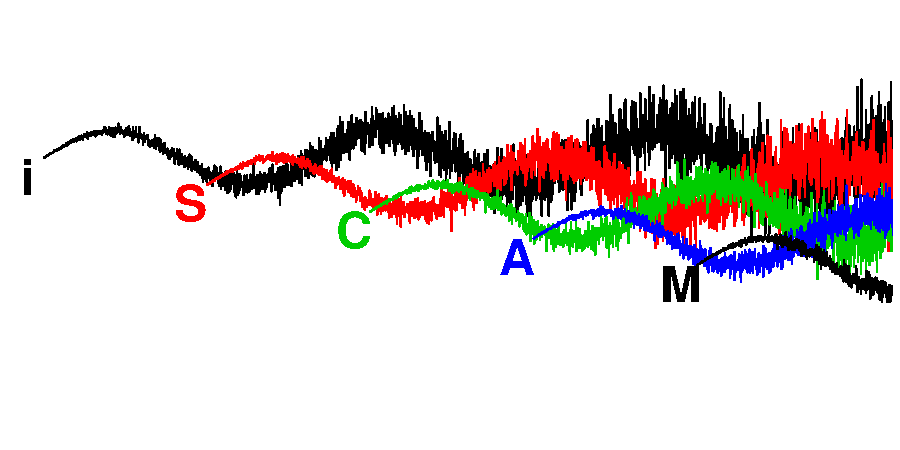
\includegraphics[height=2.53in]{iscamlogo.eps}
\vfill
\iscam\ Users Guide\\
Version 1.0\\
\vfill}
\author{Steven Martell\\
University of British Columbia\\
Fisheries Centre\\
2202 Main Mall\\
Vancouver, BC\\
V6T 1Z4\\
Canada\\ 
\texttt{s.martell@fisheries.ubc.ca}}
\date{\small{$^\copyright$  Copyright Steven Martell, \today.  All rights reserved.}}







\begin{document}

\pagenumbering{roman}
\setcounter{page}{1}
    \maketitle \thispagestyle{empty}
%    \vfill
%    \noindent\hrulefill\\
%    Draft document for peer review: Started on Wednesday, February 11, 2009\\
%    Draft document completed on Thursday, February 19, 2009\\
%    Final document completed on Wednesday, March 4, 2009.\\
%    CSAS revisions completed on Wednesday, March 11, 2009.
%    \clearpage
\thispagestyle{empty}
\clearpage


\newpage


%\begin{abstract}
%This is the abstract
%  \end{abstract}
%\clearpage


%%
 \selectlanguage{english}

    %\input{ToDoList}
%% -Executive summary material------------------------------------------

\pagenumbering{roman}
\section*{Preface}
\addcontentsline{toc}{subsection}{Preface}
This document is the users guide for the fisheries stock assessment model \iscam, or Integrated Statistical Catch Age model.  This assessment package was written by Steven Martell and may be freely used by others, but in no way am I responsible for the mess that may or may not happen if you use this software to do your job.  Although I try hard, I cannot guarantee that this application is 100\% free of bugs/coding errors so double check your own work and see if it makes sense.  If you find a bug, fix it, recompile the code and continue on.  Or let me know about the bug and I'll happily  fix it for you,  if I have time.

%%%!TEX root = /Users/stevenmartell/Documents/CURRENT PROJECTS/iSCAM-trunk/fba/BC-herring-2011/WRITEUP/BCHerring2011.tex


%\subsection*{Abstract}
%\addcontentsline{toc}{subsection}{Abstract}
%
%June 15, 2011.  Structure of this paper has changed a bit. This document will now consist of an assessment and forecast of the five major stocks and the two minor stocks.  There will be at least 5 appendixes that 1) describe the input data and the control files used for the assessment model, 2) a detailed description of \iscam, 3) a description of the methods used to develop the prior distribution, 4) simulation testing of the \iscam model, 5) moving toward the sustainable fisheries framework (see Cleary and Cox paper) and include discussion of the issues of developing an MSY-based framework for a multigear fishery with changing selectivities and natural mortality rates, and finally 6) a list of research recommendations.
%
%Summary:  Three major themes of the paper: 1) a comparing HCAM and iSCAM (where iSCAM is set up with nearly the same assumptions as 2010 HCAM assessment), 2) an iSCAM assessment with several scenarios addressing (a) q with various priors, (b) time-varying versus constant M, (c) alternative selectivity models, and (d) the interactions of all three of these confounded variables, and 3) an iSCAM assessment with the test fishery and seine roe fishery data separated into specific fleets.  The side by side comparison will examine similarities/differences between trends in biomass, fishing mortality rates, and residual fits to the spawn survey data an age-composition data.  These two models have some fundamental differences in the statistical assumptions about the catch-at-age data, so results are likely to be slightly different.  Results for all three themes will focus on reconstructing table 5 from last years assessment, with the addition of LRP and USRP to be compared with the cuttoffs and catch advice for low med and high recruitment.
%


\section*{Abstract}\addcontentsline{toc}{section}{Abstract}

Estimates of herring abundance in British Columbia (B.C.) waters  has been based on catch-age data and spawn survey abundance information.  These data are typically interpolated using a statistical catch-age framework; however, virtual methods (e.g., VPA) have been used in the past.  This document is broken into two parts: Part I deals with moving the herring assessments towards Canada's sustainable fisheries framework and introduces a new integrated statistical catch-age model for jointly estimating the abundance of Pacific herring and associated reference points to be used in the sustainable fisheries framework.  Part II of this document actually implements this new assessment framework using the data for the five major and two minor regions.  Finally, we present catch advice based on decision tables that utilize poor, average, and good age-3 recruitment forecasts.

In Part I of this document we provide a very brief description of the new assessment framework (a full technical description of the model is provided in the Appendix of this document).  We then conduct some simulation testing with perfect information to  demonstrate that the model is capable of estimating all the parameters. We further explore precision and bias in parameter estimates based on simulation data with both observation and process errors.  We then parameterize the new assessment model such that most of the assumptions of the previous assessment model (Herring Catch Age Model, or HCAM) are mostly met and compare parameter estimates and estimates of spawning stock biomass (using data from 1951:2010).  Using data from the Strait of Georgia only, we then compare alternative assumptions about the spawn survey scaling coefficient ($q$), natural mortality and selectivity, and examine how these alternative assumptions influence estimates of key parameters (unfished spawning biomass, steepness, average natural mortality).  Relaxing assumptions about $q$ and natural mortliaty rates had the largest impacts on estimated parameters.  Lastly, we compared estimates of spawning stock biomass from HCAM with the new model for all five major areas to understand the subtle differences between the assumptions in the two models \footnote{At the time of writing this document and submitting it for peer review, an error was notices in the formulation of the weight-based selectivity function for the gill net fishery.  This error has been corrected for all of the results presented in Part II, but has still to be corrected for the model comparisons in Part I of this document.  Time permitting, these comparisons will be conducted prior to the assessment meeting, and if not at least presented at the September 7, 2011 meeting.}.

In Part II of this document we present updated data from the herring fisheries and surveys in 2011, a brief description of the analytical methods used to construct the decision tables, and present the results of the application of the new assessment model to the 2011 data. New this year is a Bayesian prior for the dive survey spawn index ($q$) and the development of this prior is detailed in the appendix.  The expected value of $q$ was estimated to be 0.587 with a standard deviation of 0.155. To summarize the overall fit to the model, maximum likelihood estimates derived quantities and residuals between observed and predicted variables are used.  Retrospective analysis (i.e., the sequential removal of the most recent data) is used as a diagnostic for model misspecification.   Catch advice (decision tables) are based on the median values of random samples from the joint posterior distribution and not the maximum likelihood estimates.  Visual inspection of the trace plots from the posterior samples and pair plots were used to judge if the samples were taken from a stationary distribution. Historically catch advice was based on cuttoff values that were derived from 1996 estimates of the unfished biomass (\bo, cuttoff values are set at 0.25\bo).  This assessment provides updated estimates of \bo and presents catch advice based on new cuttoff values.  An alternative decision table, where catch advices is based on old cuttoffs, is also presented.  

Median estimates of the 2011 spawning stock biomass is as follows: Haida Gwaii (HG) --16,579 t, Prince Rupert District (PRD) -- 27,046 t, Central Coast (CC) -- 14,666 t, Strait of Georgia (SOG) 125,261 t, West Coast Vancouver Island (WCVI) 14,679 t.  Implementation of the current harvest control rule (HCR) advises no fishing in HG under poor recruitment and no fishing in CC under poor and average recruitment.  Based on the 20\% harvest rate and application of the harvest control rule the estimated maximum available harvest ranges from 4,296 t in HG to 27,690t in SOG (assuming good recruitment).  Catch advice for the minor areas is based on a 10\% fixed exploitation rate with no cuttoffs and ranges from 91 t in Area 27 (assuming poor recruitment) to 614 t in Area 2W (assuming good recruitment).

%\section*{Executive summary}\addcontentsline{toc}{section}{Executive summary}


\newpage
\tableofcontents
\addcontentsline{toc}{subsection}{Contents}
\newpage
%% -Main body of the document-------------------------------------------
\pagenumbering{arabic}
	
    \section{Introduction}
	
There are four major objectives of this paper: (1) to describe in detail an alternative integrated statistical catch-age model (iSCAM), (2) examine parameter estimation performance using iSCAM, (3) perform a side-by-side comparison of the previous HCAM and iSCAM on the five major herring stocks, and (4) explore alternative assumptions about selectivity, catchability, and natural mortality using iSCAM.  The most recent assessment of BC herring stocks was conducted in 2010 using the Herring Catch Age Model (HCAMv2) which is documented in \cite{Clear2010}.  Furthermore, a review sponsored by the Herring Research and Conservation Society (HRCS) was conducted June 17-18, 2010 in Nanaimo, BC where an expert panel addressed specific questions about the current implementation of the HCAMv2 model and suggested recommendations for each of the questions.  This paper also attempts to address some of the points brought up in the review.

BC herring are currently managed as five major stocks and 2 minor stocks (Figure \ref{Fig1}).  Annual catch advice for each of these areas is based on current estimates of stock status, and a 20\% exploitation rate if the stock is above the cutoff level for the five major stocks and a 10\% exploitation rate for the two minor stocks.  Cutoff levels for the five major stocks are based on 0.25$B_o$, and estimates of unfished biomass were established first in 1985 \citep{haist1986stock}.  These cutoffs are currently are thought to be more conservative 	than the current default Limit Reference Point of 0.4\bmsy\ \citep{dfo2006}. However, estimates of $B_o$ and MSY based reference points have not been examined for Pacific herring for some time.  In this paper we also describe the methods for updating estimates of $B_o$ and MSY based reference points using the iSCAM model framework.  We also compare estimates of MSY based reference points for the Strait of Georgia herring under the previously mentioned alternative assumptions (see point (4) in the previous paragraph).

We do not provide a detailed description of HCAMv2 in this paper and we refer the reader to \cite{schweigert2009stock} and \cite{Clear2010} for a more detailed description.  We first begin with a description of the input data required and assumptions about the data, followed by a detailed description of the analytical methods and assumptions in iSCAM. We then present the analytical methods and assumptions for exploring alternative hypotheses about selectivity, catchability and natural mortality, followed by a description of the elements that make up the joint posterior distribution (i.e., likelihoods, priors, and penalties).  Parameter estimating and quantifying uncertainty is carried out using AD Model Builder \citep{ADMB2009}.  We then explore estimation performance in iSCAM using simulation experiments where the model is used to generate simulated observations with known parameter values, then estimate parameter, and repeat this exercise a number of times to evaluate bias and precision in parameter estimates.  Finally, we present forecast of pre-fishery biomass and available harvest options using the cutoffs \cite[e.g., reproduce Table 5 in ][]{Clear2010} as well as available harvest options based on the Sustainable Fisheries Framework \citep[i.e.,][]{dfo2006} for comparison.

\begin{figure}[!tbp]
	% Requires \usepackage{graphicx}
	%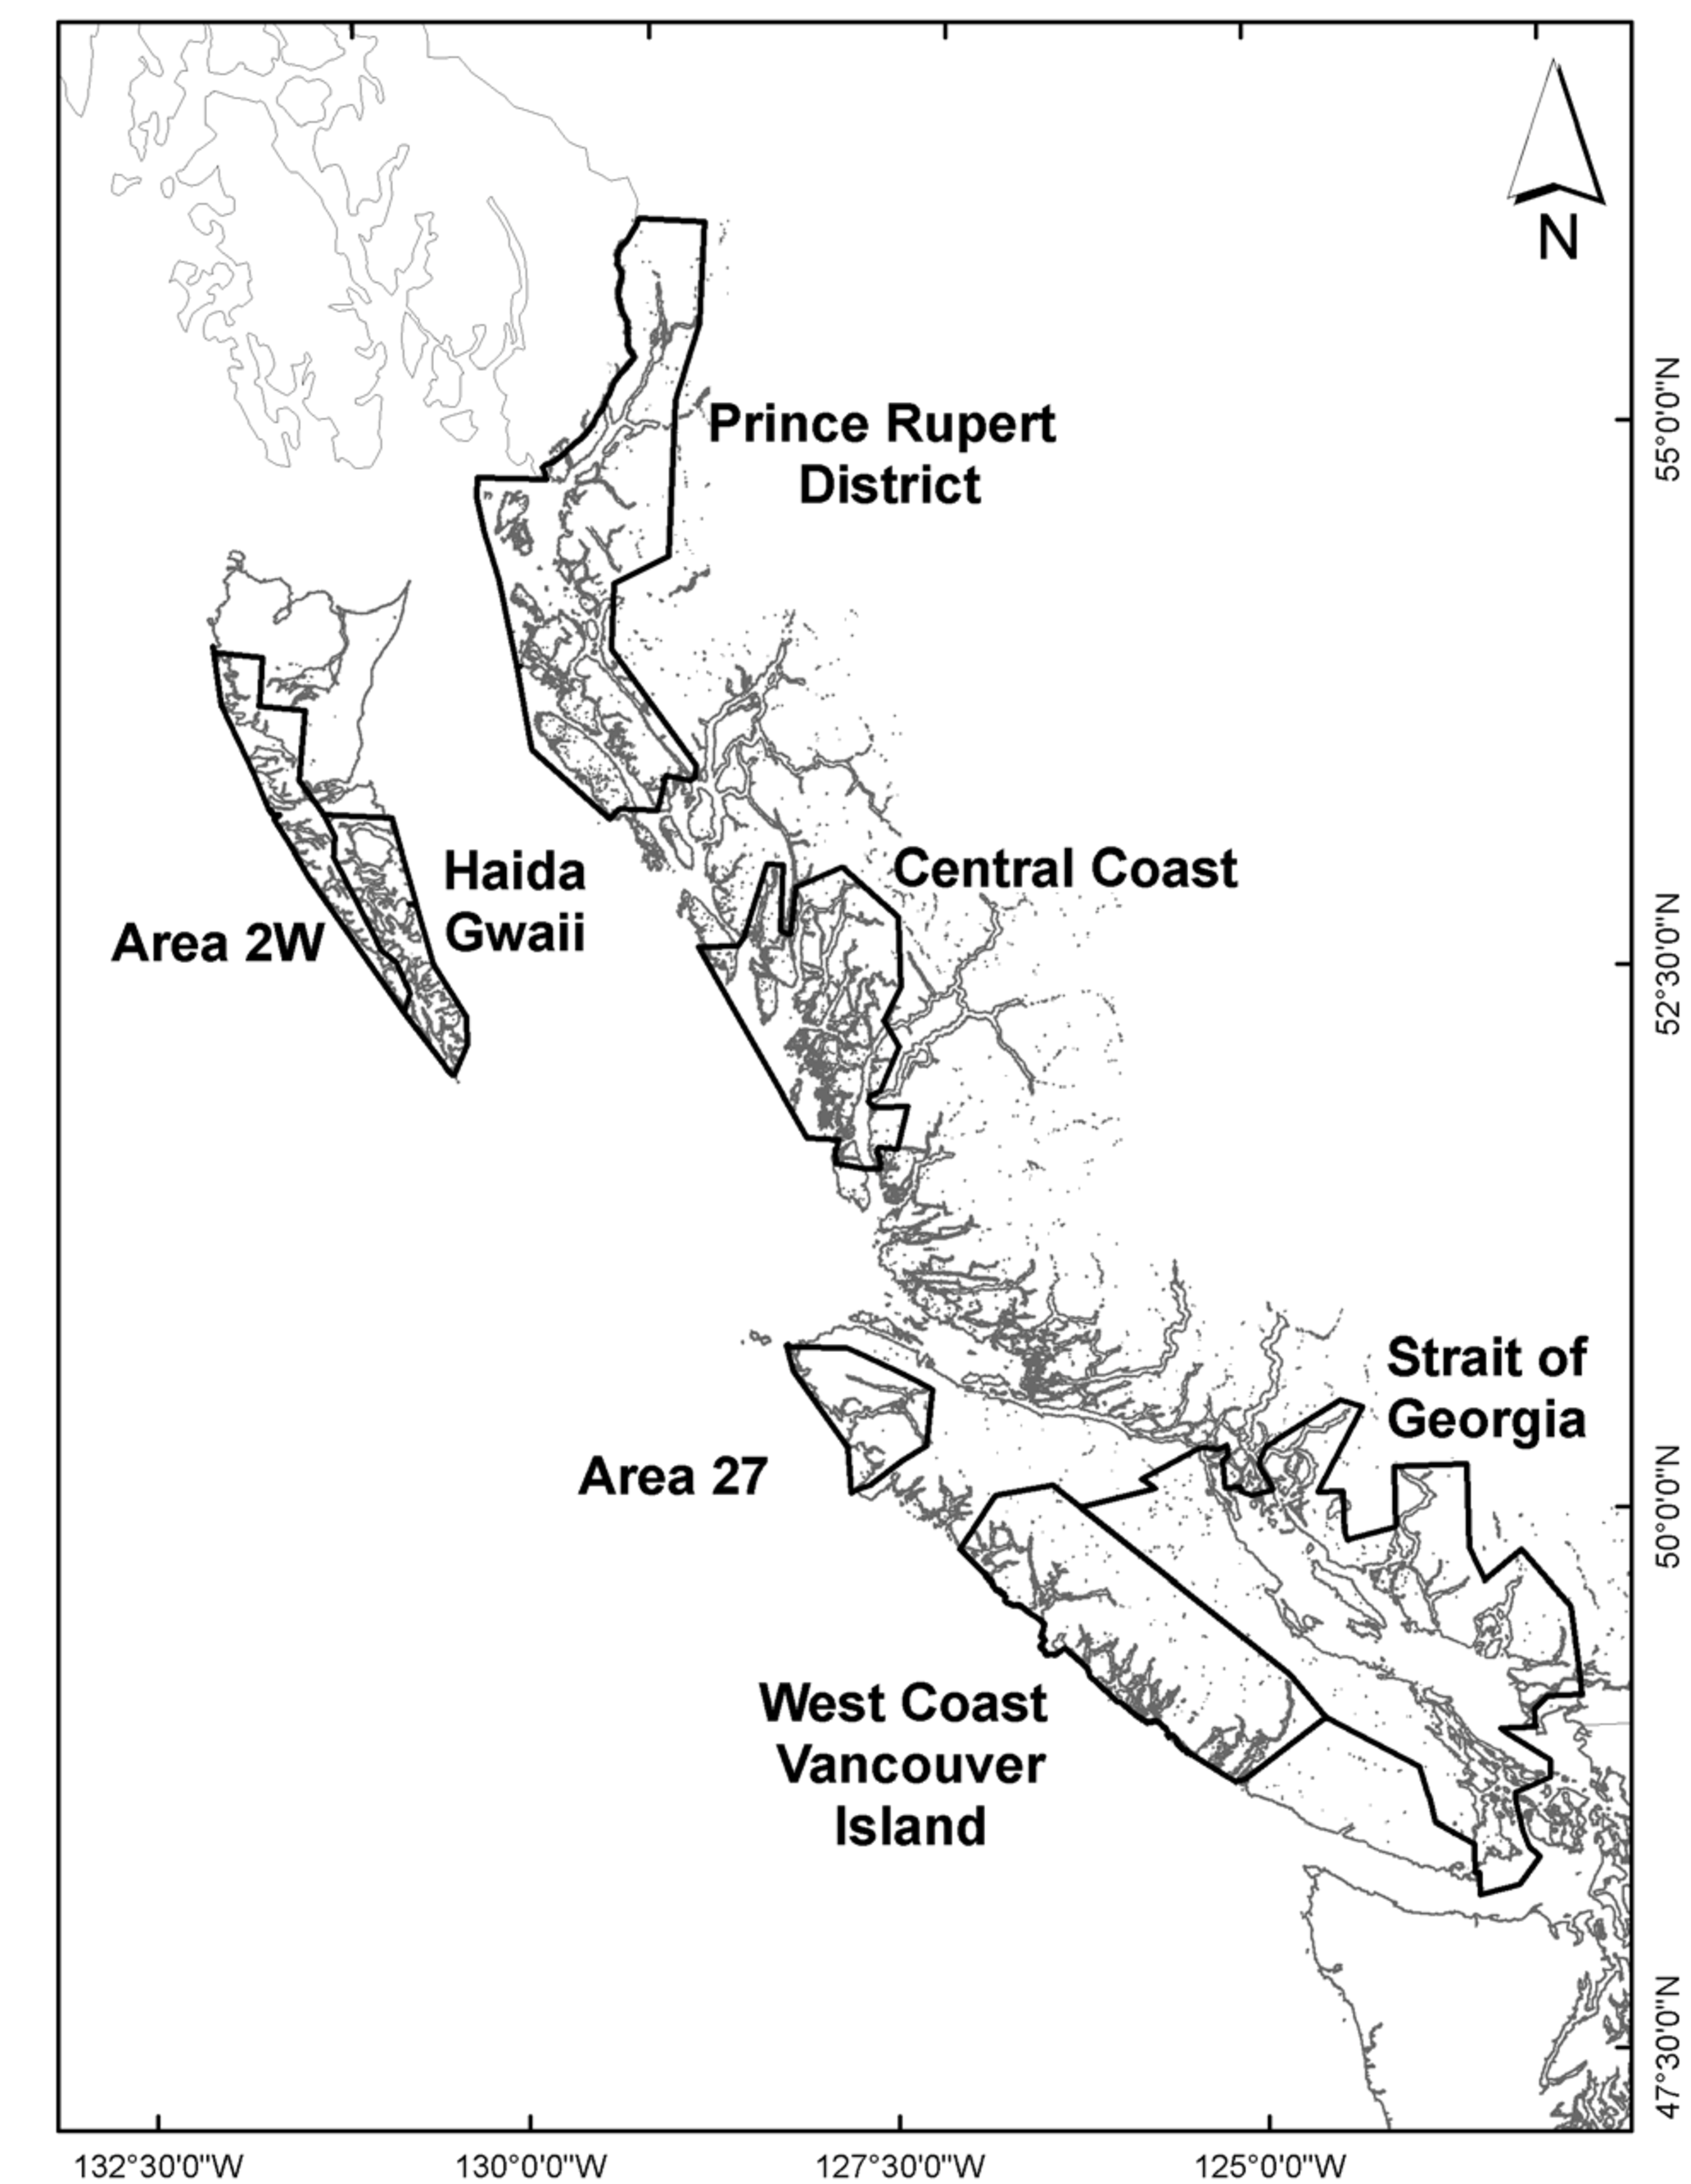
\includegraphics[width=\textwidth]{Figs/HerringAreaMap.pdf}
	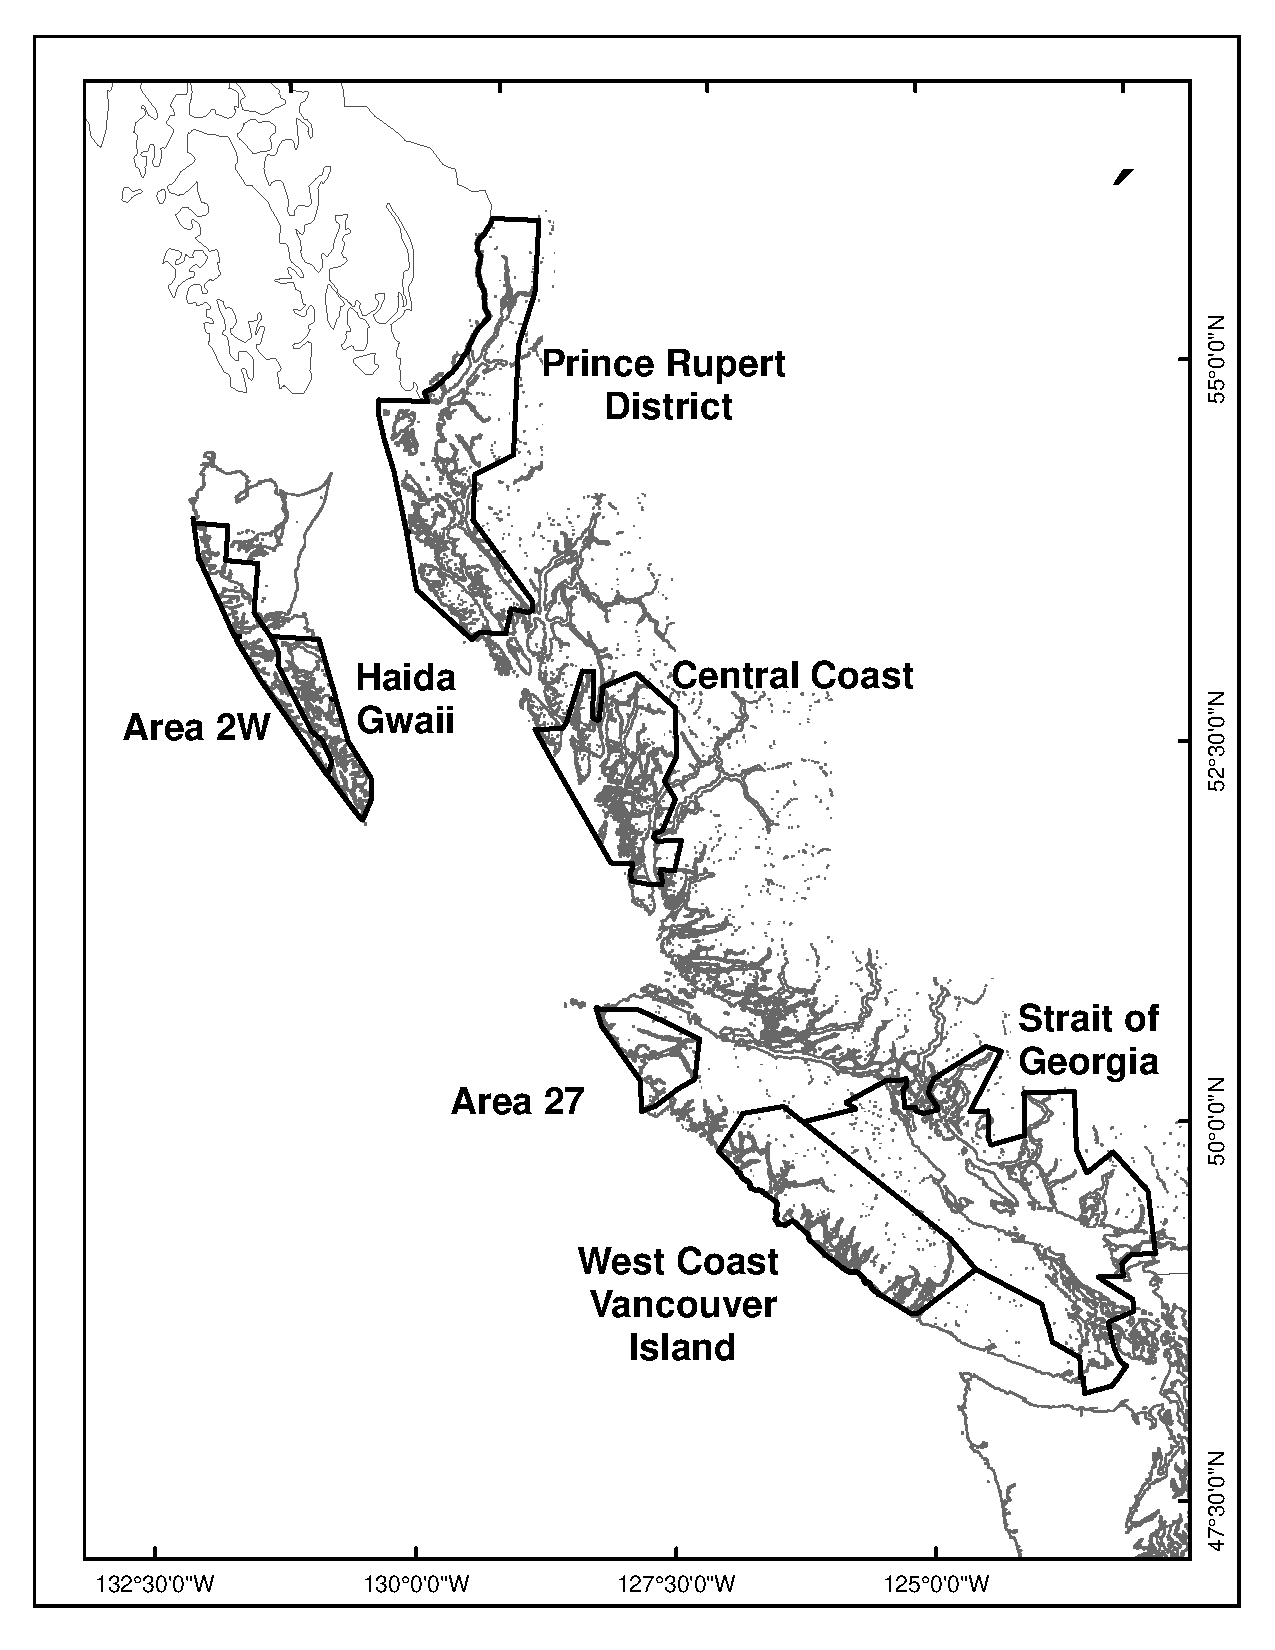
\includegraphics[width=\textwidth]{PBSfigs/Assessment_Regions_2W_27_2010_HG.pdf}
	\caption{B.C. herring major stock areas: Haida Gwaii (HG or QCI 2E), Prince Rupert District (PRD), Central
Coast (CC), Strait of Georgia (SOG), West Coast Vancouver Island (WCVI), and minor stock areas: Area 2W and
Area 27.}\label{Fig1}
\end{figure}
	
%%A reference for splines in selectivities can be found at \cite{aarts2009comprehensive}
    
\section{Running \iscam; input files \& command line options}
\begin{multicols}{2}


There are three required input files for \iscam: the \verb"iscam.dat" file, the \verb"datafile", and the \verb"controlfile".  By default when \iscam runs, the first file it looks for is the \verb"iscam.dat" file, unless otherwise specified by using the command line option \verb"-ind".  The following subsections explains the details of each of the data files.


%%%%%%%%%%%%%%%%%%%%%%%%%%%%%%%%%%%%%%%%%%%
\subsection{The \texttt{iscam.dat} file}
What is required in the \verb"iscam.dat" file is just the name of the data file and the control file, in that order.  An example is given below for the \texttt{PHake2010.dat} and \texttt{Phake2010.ctl} data and control files.
\begin{verbatim}
PHake2010.dat		#Data file name
PHake2010.ctl		#Control file name
\end{verbatim}
Note that it is necessary to have the \verb"*.dat", and \verb"*.ctl" extensions, as \iscam\ will read in the entire filename including the extension.  Also note that the \verb"#" symbol acts as a comment line, and \iscam\ will ignore the contents of the remaining line when reading in data.

%%%%%%%%%%%%%%%%%%%%%%%%%%%%%%%%%%%%%%%%%%%
\subsection{The data file}
The data file is composed of several required sections (required in the sense that they must be defined, but do not necessarily have to have data).  The first of these sections is the model dimensions.  Below is an example where the model starts in 1977 and the last year is 2009, the youngest age-group is 1 years old, and the oldest age-group is 15 years old and older (i.e., a plus group).  The total number of unique gears (including gear that samples fish in surveys is two, and last line is an integer vector that specifies if the gear is a fishery, or a survey (using 1 or 0, respectively).  For each gear you must specify 1 (a commercial fishery) or 0 (a fisheries independent survey).  Again the \verb"#" is a comment character and \iscam\ will ignore the contents after this character.  The following is an example of the model dimensions section:
\begin{verbatim}
##________________________
##____Model Dimensions____
1977		#first year of data
2009		#last year of data
1			#age of youngest age class
15			#age of plus group
2			#number of gears (ngear)
## flags for gears 
## fishery (1) or 
## survey (0) in ngears
1	0
##________________________
\end{verbatim}

The next required section is the age-schedule information pertaining to natural mortality, growth and maturity-at-age. For now, natural mortality is assumed to be age-independent.
\begin{verbatim}
## ________________________
## ___Age-schedules info___
#natural mortality rate (m)
0.23
#growth parameters (linf,k,to)
52, 0.32, 0
#length-weight allometry (a,b)
5e-6, 3.0
#maturity at age (am=log(3)/k) 
#& gm=std for logistic
3.45, 0.35
## ________________________
\end{verbatim}

Next is the time series data for the historical catch by year, fishery(ies) and survey(s).  Note that it is assumed that catch exists for each year that is specified in the model dimensions section (e.g., 1977-2009).  The first column is the year of the catch, and the subsequent columns are catch (in weight) for each fishery or survey.  Years where there are no catches (or no fishery) should be replaced by a 0.  In cases where surveys did not exist, or there were no removals (e.g., an acoustic survey), specify a zero catch for each year (row).  
\begin{verbatim}
## ________________________
#Time series data
#Observed catch 
#(1977-2009, 1,000,000 metric t)
#yr	commercial survey
1977 0.132693 0
1978 0.103639 0
1979 0.137115 0
...  omitted data for space
2008 0.321546 0
2009 0.176671 0
## ________________________
\end{verbatim}

The next section pertains to the relative abundance index, where first the number (\texttt{nit}) specified the number of independent surveys, and the next row specifies the number of observations (\texttt{nit\_nobs} ,or rows of data for each survey).  The first column is an integer vector that is used to index the survey year, the second column is the actual survey abundance index, and the third column is the gear index associated with this gear.  The fourth column is the relative weight that should be used for the index.  For example, setting wt=0 for a given year will result in omitting the data, or setting wt=2 would imply that the CV is one half of the other values.  The last column specifies the fraction of total mortality that has occurred when the survey was conducted (e.g., if the survey is conducted half way through the year then 0.5 implies that 1/2 of $Z_{t,a}$ has occurred when the survey was conducted).
\begin{verbatim}
## ________________________
#Relative Abundance index from 
#independent survey (it) 1970-2008
#nit
1
#nit_nobs
13
#iyr    it gear wt survey timing
1977 1.915  2  1   0.5
1980 2.115  2  1   0.5
1983 1.647  2  1   0.5
1986 2.857  2  1   0.5
...omitted data for space
2007 0.879  2  2   0.5
2009 1.460  2  0   0.5
## ________________________
\end{verbatim}

For age-composition information, a 3 dimensional array is used to store the information by gear-type (matrix), by year (rows of each matrix) and by age (columns of each matrix).  An example of the age composition data is shown on the following page.  

First you must specify the number of gears for which age-composition data exists.  If there are no data, then set this to 0. On  the next line you must specify the number of years of age-composition data there are for each gear type.  Next, for each gear, you must specify the first age-class of the data, and on the next row specify the oldest age-class of the data.  On the example in the next page, there are two gears, the first gear has 33 years of observations, and the second gear has 13 years of observations.  Each gear has the youngest age-class at 2 years and the oldest age-class at 15 years.  This means there are 14 columns of age-compositions for each gear type.  

The first two columns of the age-composition data refer to the year and gear type from which the data were obtained.  So in the example on the next page, the first 33 rows of the matrix (some of which is missing so it could fit on the page) corresponds to the years 1977-2009 for gear type 1, and from 1977 to 2009 every 2-3 years for gear type 2.  

The last component of the data file is an end of file ``eof'' marker, which is set to 999.  This is the last number read in from the datafile and \iscam\ checks to ensure it is 999.  If there is an error reading the datafile, \iscam\ will break and report that there was an error reading the data.


\begin{verbatim}
## ________________________
#eof
999
## ________________________
\end{verbatim}

\end{multicols}
%\begin{minipage}[b]{\linewidth}
%\centering
\begin{landscape}
\begin{footnotesize}
\begin{verbatim}
#Age composition data by year, gear (ages 2-15+)
#na_gears
2
#na_nobs
33	13
#a_sage
2	2
#a_page
15	15
#yr 	gear       V1       V2       V3       V4       V5       V6       V7       V8       V9      V10      V11      V12      V13      V14
1977    1 0.091087 0.039290 0.208628 0.028500 0.053160 0.211179 0.078270 0.079949 0.063640 0.058483 0.043761 0.029639 0.007592 0.006823
1978    1 0.022968 0.101932 0.068633 0.199094 0.033354 0.071961 0.208406 0.084622 0.072156 0.073040 0.024682 0.021006 0.013116 0.005030
1979    1 0.049457 0.089640 0.100254 0.046571 0.191908 0.071243 0.159754 0.158389 0.056370 0.037676 0.016184 0.010295 0.006469 0.005789
1980    1 0.009331 0.254593 0.042151 0.054263 0.050507 0.143816 0.065236 0.087843 0.169471 0.046122 0.037636 0.023076 0.008874 0.007079
1981    1 0.091224 0.062768 0.280898 0.012851 0.045430 0.047641 0.148751 0.062707 0.066417 0.125977 0.031183 0.012419 0.009671 0.002062
1982    1 0.181412 0.025886 0.016978 0.318964 0.032603 0.045648 0.045099 0.131034 0.027439 0.033879 0.119575 0.010972 0.006862 0.003648
1983    1 0.000322 0.327381 0.030386 0.021774 0.318861 0.034486 0.037515 0.044368 0.095257 0.024331 0.017871 0.037722 0.007340 0.002385
1984    1 0.000000 0.010415 0.546489 0.035445 0.072340 0.185115 0.023775 0.020842 0.014283 0.045333 0.009533 0.007920 0.024390 0.004121
1985    1 0.006798 0.006334 0.065169 0.607023 0.070421 0.058060 0.132423 0.011557 0.006879 0.007111 0.013539 0.002836 0.000000 0.011849
1986    1 0.111570 0.031159 0.007757 0.034088 0.485333 0.058011 0.043959 0.122124 0.022909 0.026576 0.014536 0.026627 0.004392 0.010957
1987    1 0.000000 0.264654 0.016305 0.003861 0.017893 0.540852 0.032262 0.016639 0.080708 0.003902 0.001822 0.005542 0.009811 0.005748
1988    1 0.002907 0.002881 0.325484 0.012085 0.007047 0.010794 0.464716 0.021331 0.009870 0.101698 0.001949 0.004157 0.001274 0.033806
1989    1 0.026833 0.022546 0.009612 0.452262 0.010250 0.004556 0.006132 0.394579 0.015267 0.006758 0.044542 0.000903 0.001179 0.004583
1990    1 0.048604 0.255566 0.024077 0.002273 0.251121 0.006576 0.001663 0.000990 0.323920 0.003924 0.000212 0.072414 0.000146 0.008513
1991    1 0.034754 0.176910 0.169392 0.027073 0.007271 0.316749 0.012094 0.001274 0.001349 0.206127 0.003853 0.000000 0.036791 0.006363
1992    1 0.035191 0.044184 0.126581 0.177710 0.021788 0.007533 0.344623 0.006212 0.001264 0.003920 0.198907 0.004982 0.000449 0.026655
1993    1 0.007327 0.219650 0.032109 0.141618 0.169717 0.014288 0.007544 0.287667 0.008052 0.001062 0.000425 0.104591 0.000492 0.005457
1994    1 0.000419 0.033794 0.194593 0.013819 0.121828 0.200067 0.013059 0.004773 0.307047 0.002355 0.004118 0.000280 0.096116 0.007732
1995    1 0.015172 0.001676 0.067824 0.247580 0.011946 0.076025 0.204514 0.017753 0.003065 0.259156 0.002369 0.003815 0.000000 0.089107
...	some missing data removed here to fit on page.
2005    1 0.008720 0.004799 0.070427 0.055023 0.684012 0.084118 0.021823 0.028355 0.019809 0.010432 0.008069 0.002582 0.000360 0.001470
2006    1 0.016047 0.109332 0.016100 0.086023 0.047267 0.606611 0.050565 0.017944 0.019738 0.012433 0.009263 0.004693 0.001532 0.002454
2007    1 0.135250 0.030604 0.145496 0.015585 0.070675 0.041936 0.441809 0.059055 0.018388 0.018549 0.012342 0.004254 0.004551 0.001507
2008    1 0.086419 0.307710 0.023174 0.134343 0.009449 0.035456 0.033322 0.305151 0.032058 0.010867 0.008882 0.005414 0.003330 0.004426
2009    1 0.007237 0.201241 0.298293 0.044466 0.140682 0.014182 0.025967 0.022153 0.193496 0.036166 0.005012 0.004290 0.003855 0.002961
1977    2 0.054308 0.051673 0.322415 0.029524 0.041387 0.358094 0.049372 0.036486 0.020920 0.019594 0.010201 0.003792 0.000997 0.001237
1980    2 0.004557 0.555127 0.053761 0.032569 0.026590 0.117668 0.043603 0.093838 0.037630 0.022180 0.003734 0.006424 0.001338 0.000983
1983    2 0.000265 0.785009 0.026011 0.007869 0.103384 0.016545 0.011402 0.008131 0.022356 0.005273 0.006223 0.006489 0.001042 0.000000
1986    2 0.604601 0.015879 0.002792 0.019748 0.266035 0.028628 0.022778 0.029920 0.003627 0.003812 0.000276 0.001440 0.000463 0.000000
1989    2 0.169990 0.058515 0.012874 0.526835 0.011735 0.004161 0.007554 0.179632 0.009473 0.000722 0.017782 0.000000 0.000000 0.000726
1992    2 0.089253 0.011915 0.069071 0.176823 0.021856 0.008862 0.432238 0.013086 0.007872 0.003964 0.149487 0.007606 0.000000 0.007967
1995    2 0.324964 0.043475 0.012039 0.212541 0.009810 0.032765 0.148871 0.002177 0.000000 0.158452 0.000354 0.006429 0.000000 0.048122
1998    2 0.168351 0.187074 0.157169 0.195749 0.014026 0.055093 0.087607 0.010731 0.015903 0.048868 0.003121 0.001999 0.042448 0.011861
2001    2 0.709921 0.089531 0.052761 0.056572 0.026180 0.026069 0.014190 0.008255 0.005804 0.002446 0.002162 0.004212 0.000400 0.001496
2003    2 0.029781 0.025334 0.640666 0.109500 0.027623 0.060058 0.039723 0.021949 0.022287 0.007181 0.004232 0.004367 0.003083 0.004214
2005    2 0.239916 0.024324 0.072095 0.051813 0.482518 0.052666 0.017966 0.024352 0.013884 0.011229 0.004744 0.002436 0.000323 0.001734
2007    2 0.428146 0.024375 0.101876 0.011527 0.041221 0.026044 0.289941 0.030229 0.013473 0.013191 0.007185 0.006086 0.002778 0.003928
2009    2 0.001881 0.229516 0.423131 0.024861 0.091878 0.007856 0.018074 0.024434 0.128613 0.029027 0.009417 0.005566 0.005402 0.000343
\end{verbatim}
\end{footnotesize}
\end{landscape}




%%%%%%%%%%%%%%%%%%%%%%%%%%%%%%%%%%%%%%%%%%%
\begin{multicols}{2}
\subsection{The control file (still under development)}
The first section of the control file pertains to the leading parameter vector which is summarized in Table \ref{Table.parameter.controls}.  For now, there are 6 leading parameters for which the initial values (ival) lower (lb) and upper bounds (ub) and estimation phase must be specified.  Each of these parameters also have parameters for the corresponding prior distributions defined by the prior\_type, and parameters p1 and p2.

\begin{tablehere}\caption{Controls for estimated parameters in the control file.}\label{Table.parameter.controls}
\begin{tiny}
\begin{verbatim}
## ____________________________________________________________________________ ##
##                            PACIFIC HAKE CONTROLS
## ___________________CONTROLS FOR ESTIMATED PARAMETERS________________________ ##
##  Prior descriptions:
##                      -0 uniform (0,0)
##                      -1 normal (p1=mu,p2=sig)
##                      -2 lognormal (p1=log(mu),p2=sig)
##                      -3 beta (p1=alpha,p2=beta)
##                      -4 gamma(p1=alpha,p2=beta)
## ____________________________________________________________________________ ##
6   ## npar
##  ival        lb      ub      phz     prior    p1      p2      parameter name
## ____________________________________________________________________________ ##
    1.6         -5.0    15       4       1       0.9     0.5     #log_ro/msy 
    0.65        0.2     1.0      4       3       3       2       #steepness/fmsy
    -1.469      -5.0    0.0      2       1       -1.469  0.05    #log.m
    1.6         -5.0    15       1       0       -5.0    15      #log_avgrec
    0.2         0.001   0.999    3       3       3.75    12      #rho
    1.25        0.01    500      3       4       1.01    1.01    #kappa (precision)
## ____________________________________________________________________________ ##
\end{verbatim}
\end{tiny}
\end{tablehere}
%	%\end{multicols}
%	
%	%\begin{table*}[h]
%	\begin{tablehere}
%	\caption{Controls for estimated parameters in the control file.}
%	\begin{center}
%	\begin{tiny}
%	\begin{tabular}{llllclll}
%	6 & \#npar \\
%	\hline
%	\#ival & lb & ub & phz & prior\_type & p1 & p2 & parameter name\\
%	\hline
%	1.2 & -5.0 & 15.0 & 3 & 0 & 0 & 0 & \#log\_ro or log\_msy\\
%	0.75 & 0.2 & 1.0 & 3 & 3 & 1.01 & 1.01 & \#steepness or log\_fmsy\\
%	-1.5 & -5.0 & 2.0 & -1 & 0 & 0 & 0 & \#log\_m\\
%	1.0 & -5.0 & 15.0 & 1 & 0 & 0 & 0 & \#log\_avg\_rec\\
%	0.2 & 0.001 & 0.999 & -1 & 3 & 30 & 30 & \#rho\\
%	1.25 & 0.01 & 500.0 & -1 & 4 & 1.01 & 1.01 & \#kappa (total precision)\\
%	\hline
%	\end{tabular}
%	\end{tiny}
%	\end{center}
%	\label{Table.parameter.controls}
%	\end{tablehere}
%	
%	%\begin{multicols}{2}
\subsubsection{Prior type distributions}
As of now there are 5 different prior types that can be specified and these are given by the integer values 0--4.  The following list describes the prior types and the parameter values for the distributions:
\begin{description}
\item[0] A uniform prior between lb and up. 
\item[1] A normal prior p1 = mean, and p2 = standard deviation
\item[2] A lognormal prior p1 = log(mean), and p2 = log standard deviation
\item[3] A beta prior p1 = alpha, and p2 = beta with lb and ub transformed to a 0-1 scale.
\item[4] A gamma prior with p1=alpha and p2=beta
\end{description}


\subsubsection{Selectivity controls}
The next table of numbers in the control file contains the options for selectivities for each of the gear types (both fisheries and surveys).  Currently there are 6 options implemented for selectivities in \iscam\, and the details of each are explained further in the model documentation section (see page \pageref{ModelDocSelectivity}).  The following is an excerpt from the Pacific hake control file with selectivities defined for two gears:

\begin{tiny}
\begin{verbatim}
## _________________________SELECTIVITY PARAMETERS_____________________________ ##
## OPTIONS FOR SELECTIVITY:
##      1) logistic selectivity parameters
##      2) selectivity coefficients
##      3) a constant cubic spline with age-nodes
##      4) a time varying cubic spline with age-nodes
##      5) a time varying bicubic spline with age & year nodes.
##      6) fixed logistic (set isel_type=1, and estimation phase to -1)
## Gear 1 fishery:  Gear 2 survey
## isel_type
    5        1
## Age at 50% selectivity (logistic)
    3.5      4.0
## STD at 50% selectivity (logistic)
    1.0      0.5
## No. of age nodes for each gear (0 to ignore).
    5        5
## No. of year nodes for each gear (0 to ignore).
    11       3
## Estimation phase
    2        2
## Penalty weight for 2nd differences w=1/(2*sig^2)
    12.5     12.5
## Penalty weight for dome-shaped selectivity 1=1/(2*sig^2)
    3.125    200.0
## ____________________________________________________________________________ ##
\end{verbatim}
\end{tiny}
There are two gears specified in this case, the first gear uses the time varying bicubic spline option with 5 age nodes and 11 year nodes and is estimated in phase 2 of the parameter search routine.  The second fishery (second column) is a survey with a logistic selectivity function with initial values of 4.0 and 0.5 as the mean and standard deviation that is assumed in the first phase; in the second phase these values are then treated as estimated parameters.  The last two rows of the selectivity controls defines the penalty weights used for the selectivity ogives where the 2nd differences controls the smoothness of the curve and the dome-shaped penalty limits how much the selectivity decline with older ages (dome-shaped).  Note that these two penalties are ignored for the logistic (option 1 and option 6) forms of the selectivity curve.


\subsubsection{Priors for survey catchability}
Although the scaling parameters for surveys or relative abundance indices are not directly estimated, it is possible to specify prior distributions for the conditional maximum likelihood estimates of these parameters. Priors are specified by the following four lines in the control file, there \verb"nits" is simply the number of relative abundance indices.  In the following rows, you must specify a `0' or `1' for a uniform prior or an informative prior distribution.  Note that if there is more than 1 survey, then you'll have to specify a 0 or 1 for each of the surveys (i.e., columns for each survey).  The final two rows specify the log mean of the normal prior and the standard deviation (if they prior type is uniform you must still specify these values, however they are ignored in the objective function calculation; future versions may specify lower and upper bounds of a true uniform density).  Again, in the case of multiple surveys, you must have a mean and standard deviation specified (in columns) for each of the surveys.

\begin{tiny}
\begin{verbatim}
## ____________________________________________________________________________ ##
##                             Priors for Survey q                              ##
## ____________________________________________________________________________ ##
## nits  #number of surveys
    1
## priors 0=uniform density     1=normal density
    0
## prior log(mean);
    0
## prior sd
    1
## ____________________________________________________________________________ ##
\end{verbatim}
\end{tiny}


\subsubsection{Other miscellaneous controls}
The following is an ordered list of controls that turn various switches on and off or set up alternative structural assumptions such as Ricker recruitment or time varying natural mortality rates in \iscam.  It's also a place holder to add additional features to \iscam\ as the model continues to evolve over time. The following is an ordered list describing in more detail each of the miscellaneous controls.

\begin{enumerate}

	\item The first row of the miscellaneous controls is a flag that turns on and off the verbose output of \iscam.

	\item Switch between Beverton-Holt  recruitment \eqref{T4.12} and Ricker recruitment \eqref{T4.13}.
	
	\item The assumed standard deviation (in log space) in the observed catch in all phases except the last phase of the parameter estimation scheme.  Note that this value must be greater than 0.  Slightly larger values (say 0.05) will speed up convergence in earlier phases.
	
	\item The assumed standard deviation (in log space) in the observed catch in the last phase of the parameter estimation scheme.  Note that this value must be greater than 0.  Slightly smaller values (say 0.01) will increase precision in the estimates of F but generally slow down convergence.
		
	\item The next item is a flag to initialize the model at an unfished state in the initial year, otherwise, \iscam\ estimates the numbers at age in the first year.
	
	\item Age-composition data are pooled into plus groups if the observed proportions-at-age are less than the specified percentage (e.g., $<$1\% in the example control file below).  See description of age-cmposition data, specifically the last paragraph in section \ref{agecomps} on page \pageref{agecomps}.
	
	\item During the initial phases of the parameter estimation, a large penalty is used to regularize the estimates of the annual fishing mortality rates and then in the last phase this penalty is relaxed.  The penalty is on deviations from the average fishing mortality rate (0.20 in the example below) for all fishing fleets.  
	
	\item The assumed standard deviation (in log space) in the fishing mortality rate penalty in the initial phases.
	
	\item The assumed standard deviation (in log space) in the fishing mortality rate in the last phase, (should be a large value (e.g., 5 or greater), otherwise the penalty could reduce the true variation in the estimated $F_t$'s.
	
	\item The option to estimate changes in natural mortality rates via a random walk process is implemented by selecting a positive phase (negative values imply a constant $M$) and annual deviations in $M$ are not estimated.
	
	\item  If annual deviations in natural mortality are estimated, then the standard deviation for the normal prior for deviations in $M_t$ are specified here.
\end{enumerate}




\begin{tiny}
\begin{verbatim}
## _______________________OTHER MISCELLANEOUS CONTROLS_________________________ ##
0           ## verbose ISCAM output (0=off, 1=on).
1           ## recruitment model (1=beverton-holt, 2=ricker).
0.05        ## std in observed catches in initial phases.
0.01        ## std in observed catches in last phase.
0           ## Assume unfished in first year (0=FALSE, 1=TRUE).
0.01        ## Minimum proportion to consider in age-proportions for dmvlogistic.
0.20        ## Mean fishing mortality for regularizing the estimates of Ft.
0.01        ## std in mean fishing mortality in initial phases.
5.00        ## std in mean fishing mortality in last phase.
-1          ## phase for estimating m_deviations (use -1 to turn off mdevs).
0.1         ## std in deviations for natural mortality.
## ____________________________________________________________________________ ##

\end{verbatim}
\end{tiny}


\end{multicols}

%\begin{figure*}[b]
%	% Requires \usepackage{graphicx}
%	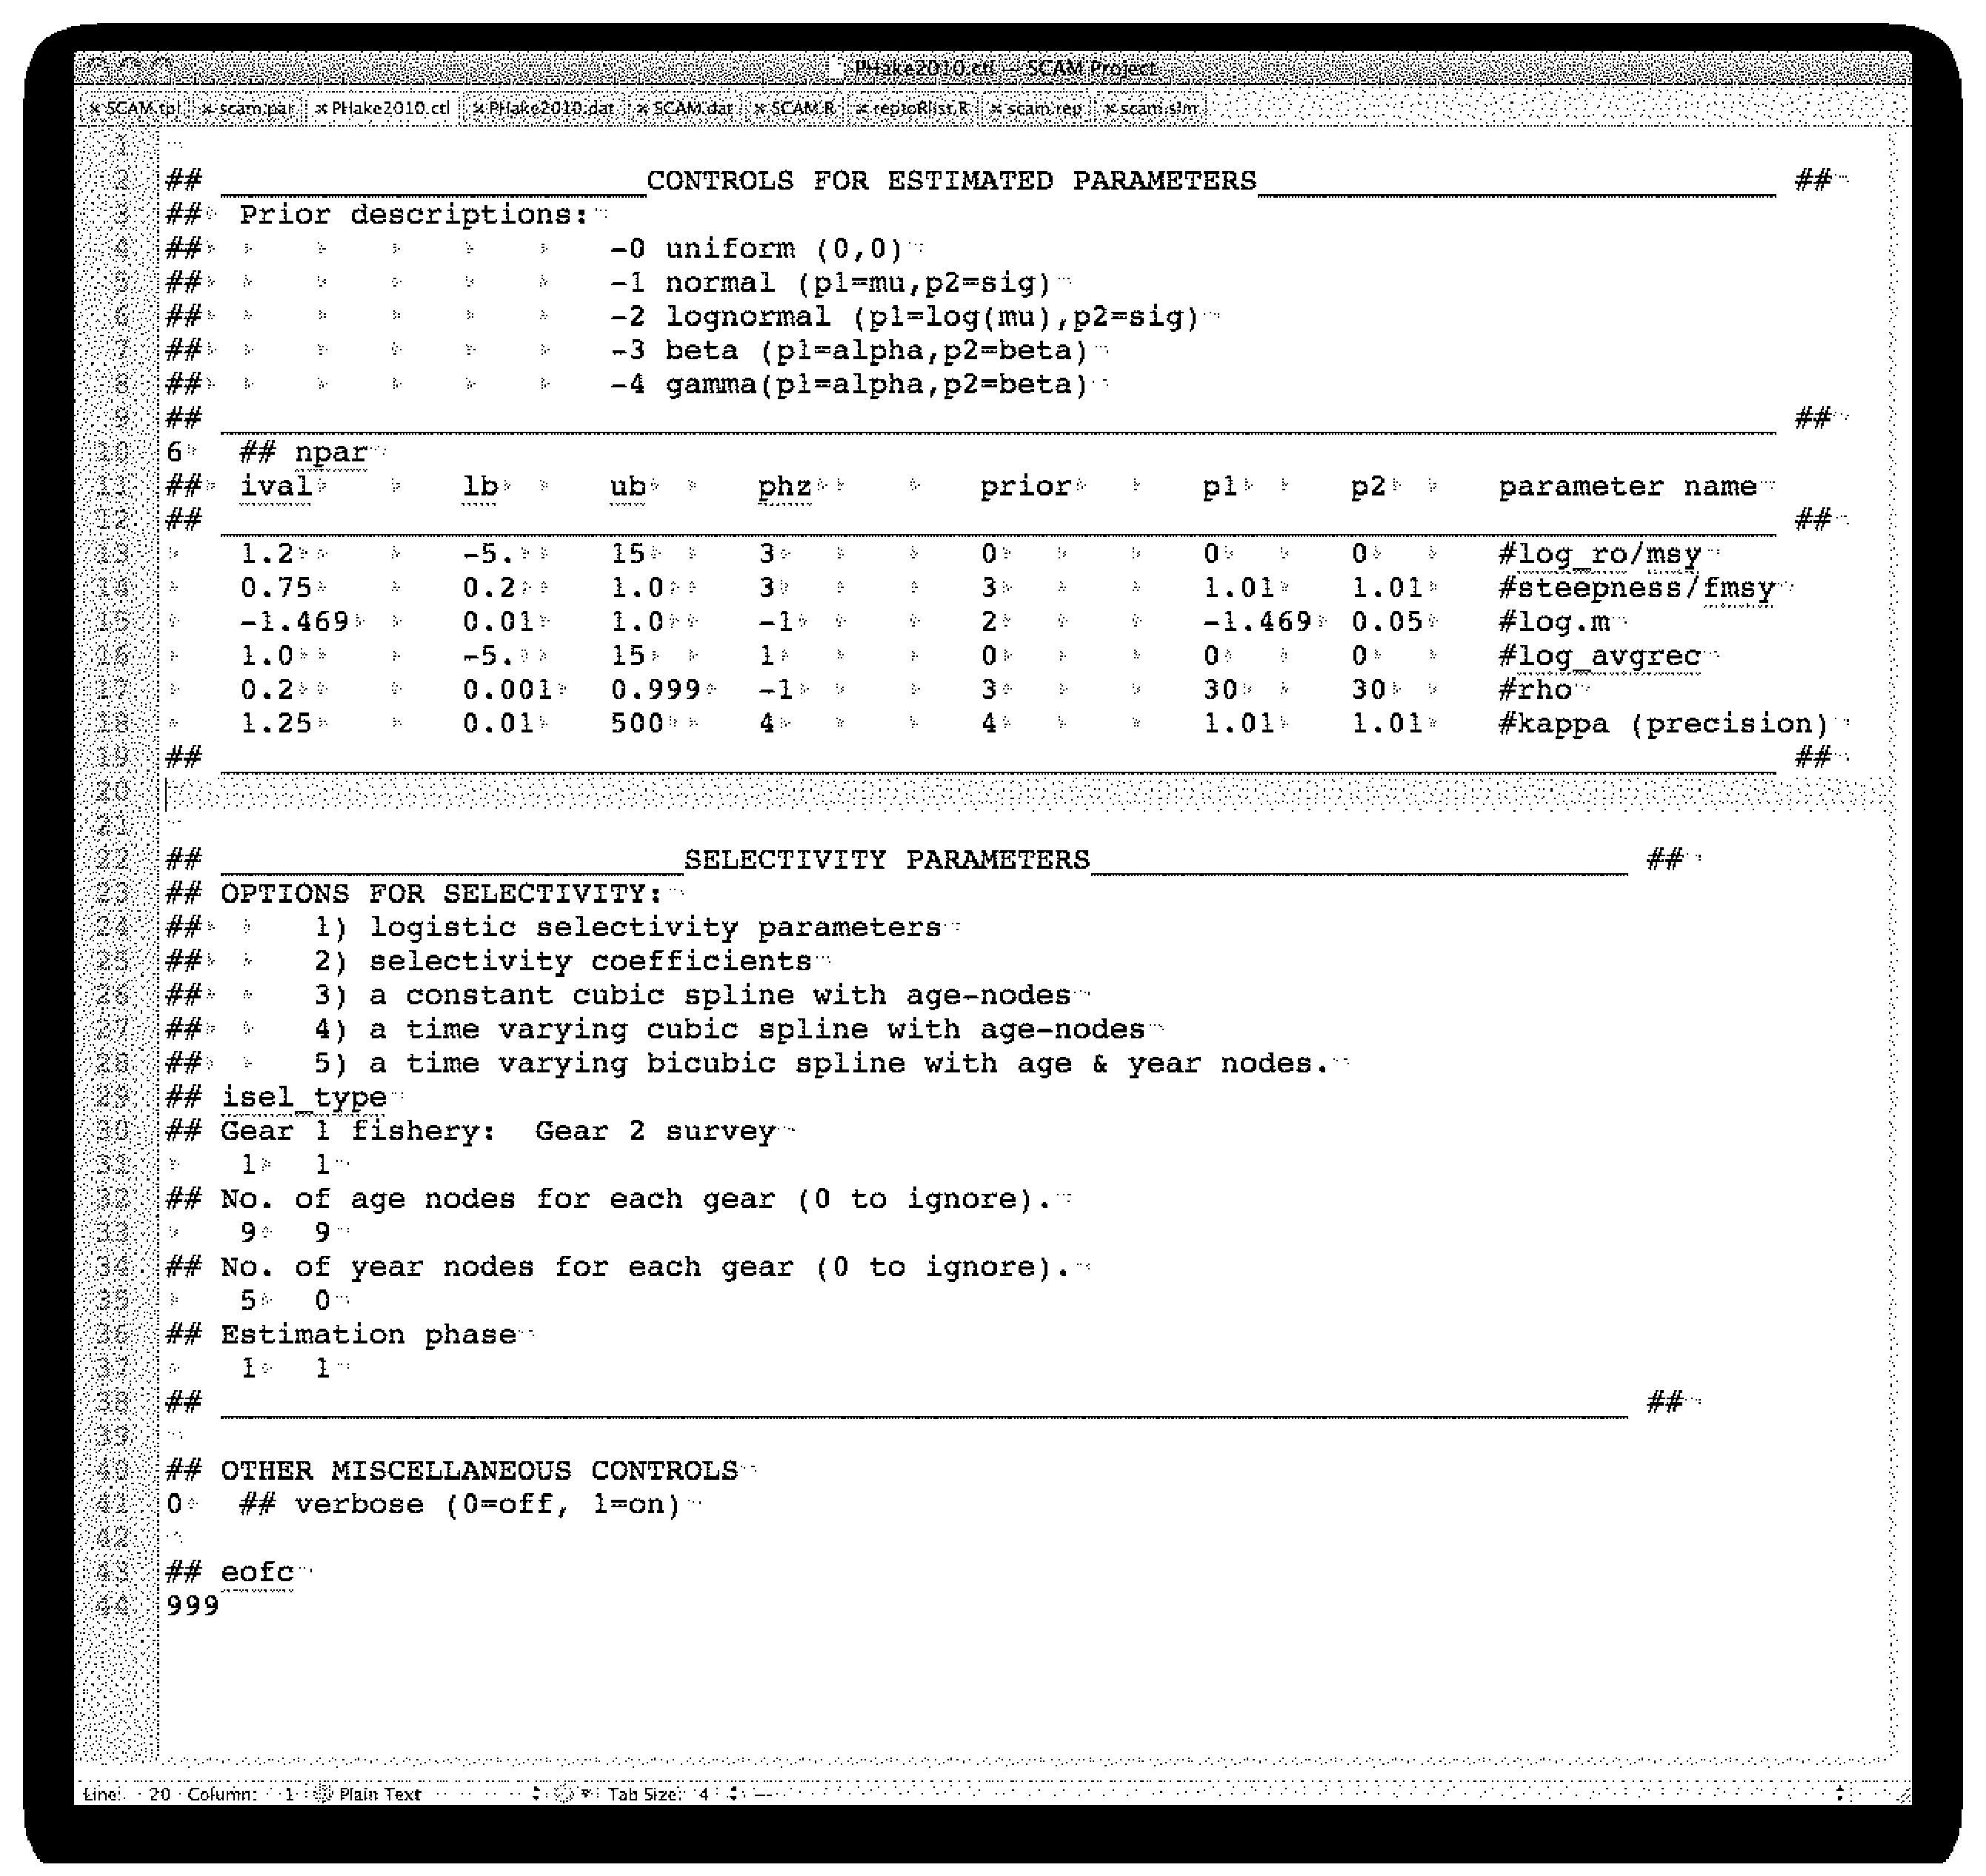
\includegraphics[width=\textwidth]{sc1.eps}\\
%	\caption{A screen shot of the example control file.}\label{Fig.control.file}
%\end{figure*}



\begin{multicols}{2}

\subsection{Command line options}
Currently there are two custom command line options available in \iscam\ in addition to the standard command line options provided by the AD Model Builder libraries (see help command line options -? for more information on the ADMB command line options). 

The custom command line options are:
\begin{description}
\item[-sim N] use this option turn the model into a simulation model, where N is the random number seed.

\item[-retro N] use the option for retrospective analysis where the last N years of data are ignored in the likelihood calculations.
\end{description}

There two random number seeds for the simulation model that the user should be aware of.  The first is if the random number seed is set to 000, then \iscam\ will actually simulate data with no errors whatsoever.  That is, the values of $\sigma$ and $\tau$ (observation error and process errors, respectively) will be set equal to 0 and the simulation model will run as a deterministic model with no observation errors in the relative abundance index or age composition data.  This option allows the user to check to ensure that the model parameters are in fact estimable with perfect information.


The second unique random seed number is 99, and this seed number is used for the simulation example in this manuscript.  It specifies a unique time-varying selectivity curve for the commercial fishery that goes from dome-shaped to asymptotic.

\subsubsection{Running the simulation model}

Again, one of the first steps in conducting any assessment should be to first run the model on simulated data with no error to be certain that the model is capable of estimating the specified model parameters.  To do so in \iscam\, the user simply needs to specify the command line option of \texttt{-sim 000}, where the `000' argument specifically instructs \iscam\ not to add any random variation to the observation or process errors.  Invoking this command line option will run \iscam\ as normal, where the data from the data file is first read into memory, then the information from the control file is then read in.  However, before proceeding straight into the non-linear parameter estimation procedure, \iscam\ first runs a simulation model based on the specified parameters listed in the control file.  This simulation model will then replace the existing data in memory with simulated data, then perform the non-linear parameter estimation procedure and attempt to estimate the model parameters.  If all is working well the estimated parameters listed in the parameter file should be very close, if not exactly, to the initial values specified in the control file.




\end{multicols}

    \section{Model Documentation}
\begin{multicols}{2}
The section contains the documentation in mathematical form of the underlying age-structured model, and its steady state version that is used to calculate reference points, the observation models used in predicting observations, and the components of the objective function that formulate the statistical criterion (i.e., the objective function) that is used to estimate model parameters.  All of the model equations are laid out in tables and are intended to represent the order of operations, or pseudocode, in which to implement the model.  \iscam\ was implemented in AD Model Builder version 9.0.0 \citep{otterResearch,ADMB2009}.
\end{multicols}

\subsection{Age-structured population model: equilibrium considerations}
\begin{multicols}{2}
For the steady-state conditions represented in Table \ref{Table2}, we assume the parameter vector $\Theta$ in \eqref{T2.1} is unknown and would eventually be estimated by fitting \iscam\ to time series data.  For a given set of growth parameters and maturity-at-age parameters defined by \eqref{T2.3}, growth is assumed to follow von Bertalanffy \eqref{T2.4}, mean weight-at-age is given by the allometric relationship in \eqref{T2.5}, and the age-specific vulnerability is given by a logistic function \eqref{T2.6}.  Note, however, there are alternative selectivity functions implemented in \iscam, the logistic function used here is simply for demonstration purposes.  Mean fecundity-at-age is assumed to be proportional to the mean weight-at-age of mature fish, where maturity at age is specified by the parameters $\dot{a}$ and $\dot{\gamma}$ for the logistic function.

Survivorship for unfished and fished populations is defined by \eqref{T2.8} and \eqref{T2.9}, respectively.  It is assumed that all individuals ages $A$ and older (i.e., the plus group) have the same total mortality rate.  The incidence functions refer to the life-time or per-recruit quantities such as spawning biomass per recruit ($\phi_E$) or vulnerable biomass per recruit ($\phi_b$).  Note that upper and lower case subscripts denote unfished and fished conditions, respectively.  Spawning biomass per recruit is given by \eqref{T2.10}, the vulnerable biomass per recruit is given by \eqref{T2.11} and the per recruit yield to the fishery is given by \eqref{T2.11b}.  Unfished recruitment is given by \eqref{T2.12} and the steady-state equilibrium recruitment  for a given fishing mortality rate $F_e$ is given by \eqref{T2.13}.  Note that in \eqref{T2.13} we assume that recruitment follows a Beverton-Holt model of the form:
\[
R_e=\frac{s_o R_e \phi_e}{1+\beta R_e \phi_e}
\]
where
\[
s_o = \kappa/\phi_E,
\]
\[
\beta = \frac{(\kappa-1)}{R_o\phi_E},
\]
which simplifies to \eqref{T2.13}.
The equilibrium yield for a given fishing mortality rate is \eqref{T2.14}.  These steady-state conditions are critical for determining various reference points such as \fmsy\ and \bmsy.  









%%%%%%%%%%%%%%%%%%%%%%%%%%%%%%%%%%%%%%%%%%%%%%%%%%%%%%%%%%%%%%%%%%%%%%
%%%%%%%%%%%%%%%%%%%%%%%%%%%%%%%%%%%%%%%%%%%%%%%%%%%%%%%%%%%%%%%%%%%%%%
\begin{tablehere}
  %\centering
\caption{Steady-state age-structured model assuming unequal
vulnerability-at-age, age-specific natural mortality, age-specific
fecundity and Beverton-Holt type recruitment.}\label{Table2} 
\tableEq
    \begin{gather}
           \hline
        \mbox{Parameters} \nonumber \\
            \Theta = (B_o,\kappa,M_a,\hat{a},\hat{\gamma}) \label{T2.1}\\
            B_o>0; \kappa > 1; M_a > 0\\
            \Phi = (l_\infty, k, t_o,a,b,\dot{a},\dot{\gamma}) \label{T2.3}\\[1ex]
        %%
        %%
        \mbox{Age-schedule information} \nonumber\\
            l_a=l_\infty(1-\exp(-k(a-t_o)))\label{T2.4}\\
            w_a=a(l_a)^b \label{T2.5}\\
            v_a=(1+\exp(-(\hat{a}-a)/\gamma))^{-1} \label{T2.6}\\
            f_a=w_a(1+\exp(-(\dot{a}-a)/\dot{\gamma}))^{-1} \label{T2.7}\\[1ex]
        %%
        %%
        \mbox{Survivorship} \nonumber\\
            \iota_a=\begin{cases} 1, \quad a=1      \label{T2.8} \\
            \iota_{a-1}e^{-M_{a-1}},\quad a>1\\
            \iota_{a-1}/(1-e^{-M_a}),\quad a=A \end{cases}\\
            \hat{\iota}_a=\begin{cases} 1, \quad a=1\\
            \hat{\iota}_{a-1}e^{-M_{a-1}-F_e v_{a-1}},\quad a>1\\
            \hat{\iota}_{a-1}e^{-M_{a-1}-F_e v_{a-1}}/(1-e^{-M_{a}-F_e v_{a}}),\quad a=A
            \end{cases} \label{T2.9}\\[1ex]
        %%
        %%
        \mbox{Incidence functions} \nonumber \\
            \phi_E=\sum_{a=1}^\infty \iota_a f_a, \quad
            \phi_e=\sum_{a=1}^\infty \hat{\iota}_a f_a \label{T2.10}\\
            \phi_B=\sum_{a=1}^\infty \iota_a w_a v_a, \quad
            \phi_b=\sum_{a=1}^\infty \hat{\iota}_a w_a v_a \label{T2.11}\\
            \phi_q=\sum_{a=1}^\infty
                \frac{ \hat{\iota}_a w_a v_a}{M_a+F_ev_a}
                \left(1-e^{(-M_a-F_ev_a)}\right) \label{T2.11b} \\[1ex]
        %%
        %%
        \mbox{Steady-state conditions} \nonumber \\
        R_o=B_o/ \phi_B \label{T2.12}\\
        R_e=R_o\frac{\kappa-\phi_E/\phi_e}{\kappa-1} \label{T2.13}\\
        %%C_e=R_e \phi_b \frac{F_e}{Z_e}(1-\exp(-Z_e))\label{T2.14} \B \\
        C_e=F_e R_e \phi_q\label{T2.14} \\[1ex]
        \hline \hline \nonumber
    \end{gather}
    \normalEq
\end{tablehere}
%%%%%%%%%%%%%%%%%%%%%%%%%%%%%%%%%%%%%%%%%%%%%%%%%%%%%%%%%%%%%%%%%%%%%%
%%%%%%%%%%%%%%%%%%%%%%%%%%%%%%%%%%%%%%%%%%%%%%%%%%%%%%%%%%%%%%%%%%%%%%

\subsubsection{MSY based reference points}
\iscam\ calculates \fmsy\ based reference points by taking finding the value of $F_e$ that results in the zero derivative of \eqref{T2.14}.  This is accomplished numerically using a Newton-Raphson method where an initial guess for \fmsy\ is set equal to 1.5$M$, then use \eqref{eq1.1} to iteratively find \fmsy.  Note that the partial derivatives in \eqref{eq1.1} can be found in Table \ref{Table3}.

\begin{align}\label{eq1.1}
    F_{e+1}&=F_e - 
    \dfrac{ \dfrac{\partial C_e}{\partial F_e}}
    { \dfrac{\partial^2 C_e}{\partial F_e}}\\
    \mbox{where}\nonumber\\
     \frac{\partial C_e}{\partial F_e} &=
    R_e \phi_q
    + F_e \phi_q \dfrac{\partial R_e}{\partial F_e}
    + F_e R_e \dfrac{\partial \phi_q}{\partial F_e} \nonumber\\
    \frac{\partial^2 C_e}{\partial F_e} &=
    \phi_q \dfrac{\partial R_e}{\partial F_e}
   +  R_e \dfrac{\partial \phi_q}{\partial F_e}\nonumber
%    \frac{R_e \phi_q
%    + F_e \phi_q \dfrac{\partial R_e}{\partial F_e}
%    + F_e R_e \dfrac{\partial \phi_q}{\partial F_e}}
%    {\phi_q \dfrac{\partial R_e}{\partial F_e}
%    +  R_e \dfrac{\partial \phi_q}{\partial F_e}}.
\end{align}

The algorithm usually converges in less than 10 iterations depending on how close the initial guess of \fmsy\ is to the true value.  A maximum of 20 iterations are allowed in \iscam, however, if $\frac{\partial C_e}{\partial F_e}<1e-5$ the algorithm stops.  Note also, that this is only performed on data type variables and not differentiable variables within AD Model Builder.

Given an estimate of \fmsy, other reference points such as MSY are calculated use the equations in Tabel \ref{Table2} where each of the expressions is evaluated at \fmsy.  A graphical representation of MSY based reference points for two alternative values of the recruitment compensation parameter $\kappa$ is show in Figure \ref{Fig1}.

\begin{figurehere}
  % Requires \usepackage{graphicx}
  \centering
  \psfrag{Re}{$R_e$}
  \psfrag{Fe}{$F_e$}
  \psfrag{Ce}{$C_e$}
  \psfrag{Be}{$B_e$}
  \psfrag{F}{$F_e$}
  \psfrag{SPR}{$\phi_e/\phi_E$}
 %\psfrag{k=12}{$\kappa=12$}
  %\psfrag{k=4}{$\kappa=4$}
  \includegraphics[width=\columnwidth]{iscamFigs/Fig1.Quadplot.eps}\\
  \caption{Equilibrium yield (a), recruits (b), biomass (c) and
spawner per recruit ($\phi_e/\phi_E$) (d) versus instantaneous
fishing mortality $F_e$ for two different values of the recruitment
compensation ratio ($\kappa=12$ solid lines, $\kappa=4$ dashed
lines). Vertical lines in each panel correspond to \fmsy\ and
horizontal lines correspond to various reference points that would
achieve MSY.}\label{Fig1}
\end{figurehere}


%%%%%%%%%%%%%%%%%%%%%%%%%%%%%%%%%%%%%%%%%%%%%%%%%%%%%%%%%%%%%%%%%%%%%%
%%%%%%%%%%%%%%%%%%%%%%%%%%%%%%%%%%%%%%%%%%%%%%%%%%%%%%%%%%%%%%%%%%%%%%
\begin{tablehere}
  \centering
\caption{Partial derivatives, based on components in Table
\ref{Table2}, required for the numerical calculation of \fmsy\ using \eqref{eq1.1}.}\label{Table3} \tableEq
    \begin{gather}
        \hline
        \mbox{Mortality \& Survival} \nonumber \\
        Z_{a}=M_a+F_ev_a \label{T3.1} \\
        S_{a}=1-e^{-Z_a}\label{T3.2}\\[1ex]
        %%
        %%
        \mbox{Partial for survivorship} \nonumber \\
        \frac{\partial \hat{\iota}_a}{\partial F_e} =
        \begin{cases}
          0,& a=1 \label{T3.3}\\
          e^{-Z_{a-1}}\left(\dfrac{\partial \hat{\iota}_{a-1}}{\partial F_e}
           -\hat{\iota}_{a-1}v_{a-1}\right),& a>1
        \end{cases} \\[1ex]
        %%
        %%
        \mbox{Partials for incidence functions} \nonumber \\
        \frac{\partial \phi_e}{\partial F_e}=
            \sum_{a=1}^\infty f_a \frac{\partial \hat{\iota}_a}{\partial
            F_e} \label{T3.4}\\
        %%
        %%
        \frac{\partial \phi_q}{\partial F_e}=
            \sum_{a=1}^\infty \frac{w_av_a S_a}{Z_a}
             \frac{\partial \hat{\iota}_a}{\partial F_e}
             +\frac{\hat{\iota}_a w_av_a^2}{Z_a}\left(e^{-Z_a}-\frac{S_a}{Z_a} \right) \label{T3.5}\\[1ex]
        %%
        %%
        \mbox{Partial for recruitment} \nonumber\\
        \frac{\partial R_e}{\partial F_e}=\frac{R_o}{\kappa-1}
        \frac{\phi_E}{\phi_e^2} \frac{\partial \phi_e}{\partial
        F_e} \label{T3.6}\\[1ex]
        \hline \hline \nonumber
    \end{gather}

    \normalEq
\end{tablehere}
%%%%%%%%%%%%%%%%%%%%%%%%%%%%%%%%%%%%%%%%%%%%%%%%%%%%%%%%%%%%%%%%%%%%%%
%%%%%%%%%%%%%%%%%%%%%%%%%%%%%%%%%%%%%%%%%%%%%%%%%%%%%%%%%%%%%%%%%%%%%%


\end{multicols}



\subsection{Age-structured population model: state-dynamics}
\begin{multicols}{2}
The estimated parameter vector in \iscam\ is defined in \eqref{T4.1}, where $R_0, \kappa$ and $M$ are the leading unknown population parameters that define the overall population scale in the form of unfished recruitment and productivity in the form of recruitment compensation and natural mortality.  The total variance $\vartheta^2$ and the proportion of the total variance that is associated with observation errors $\rho$ are also estimated, then the variance is partitioned into observation errors ($\sigma^2$) and process errors ($\tau^2$) using \eqref{T4.2}.

The unobserved state variables \eqref{T4.3} include the numbers-at-age year year $t$ ($N_{t,a}$), the spawning stock biomass ($B_t$) and the total age-specific total mortality rate ($Z_{t,a}$).

The initial numbers-at-age in the first year \eqref{T4.4} and the annual recruits \eqref{T4.5} are treated as estimated parameters and used to initialize the numbers-at-age matrix.  Age-specific selectivity for gear type $k$ is a function of the selectivity parameters $\gamma_k$ \eqref{T4.6}, and the annual fishing mortality for each gear is the product of the average fishing mortality ($\bar{F}_k$) and the annual fishing mortality deviation that has the additional constraint of summing to zero for each gear type ($\delta_{k,t}$, where $\sum_t \delta_{k,t}=0$).

State variables in each year are updated using equations \ref{T4.8}--\ref{T4.11}, where the spawning biomass is the product of the numbers-at-age and the mature biomass-at-age \eqref{T4.8}.  The total mortality rate is given by \eqref{T4.9}, and the total catch (in weight) for each gear is given by \eqref{T4.10} assuming that both natural and fishing mortality occur simultaneously throughout the year.  The numbers-at-age are propagated over time using \eqref{T4.11}, where members of the plus group (age $A$) are all assumed to have the same total mortality rate.  

Recruitment to age $k$ can follow either a Beverton-Holt model \eqref{T4.12} or a Ricker model \eqref{T4.13} where the maximum juvenile survival rate in either case is defined by $\kappa/\phi_E$.  For the Beverton-Holt model, $\beta$ is derived by solving \eqref{T4.12} for $\beta$ conditional on estimates of $\kappa$ and $R_o$:
\[
\beta = \frac{\kappa-1}{R_o \phi_E},
\]
and for the Ricker model this is given by:
\[
\beta = \frac{\ln(\kappa)}{R_o \phi_E}
\]

%%%%%%%%%%%%%%%%%%%%%%%%%%%%%%%%%%%%%%%%%%%%%%%%%%%%%%%%%%%%%%%%%%%%%%%%
%%%%%%%%%%%%%%%%%%%%%%%%%%%%%%%%%%%%%%%%%%%%%%%%%%%%%%%%%%%%%%%%%%%%%%%%
\begin{tablehere}
  \centering
\caption{Statistical catch-age model using the Baranov catch
equation and $C^*$ and $F^*$ as leading parameters.}\label{Table4}
\tableEq
    \begin{align}
        \hline \nonumber \\
        &\mbox{Estimated parameters} \nonumber\\
        \Theta &= (R_0,\kappa,\bar{R},\rho,\vartheta^2,\gamma_{k},\bar{F}_k,\delta_{k,t},\{\omega_t\}_{t=1-A}^{t=T}) \label{T4.1}\\
        \sigma^2&=\rho /\vartheta^2, \quad
        \tau^2=(1-\rho)/\vartheta^2\label{T4.2}\\[1ex]
        %\vartheta^2=\sigma^2+\tau^2, \quad
        %\rho=\frac{\sigma^2}{\sigma^2+\tau^2}\label{T4.3}\\[1ex]
        %%
        %%
        &\mbox{Unobserved states} \nonumber\\
        &N_{t,a},B_t,Z_{t,a}	\label{T4.3}\\
	%%
	%%	        
        &\mbox{Initial states} \nonumber\\
        %v_a=\left[1+e^{-(\hat{a}-a)/\hat{\gamma}}\right]^{-1}\label{T4.7}\\
        N_{t,a}&=\bar{R}e^{\omega_{t-a}} \exp(-M)^{(a-1)};\quad t=1;  2\leq a\leq A\label{T4.4}\\
        N_{t,a}&=\bar{R}e^{\omega_{t}} ;\quad 1\leq t\leq T;  a=1\label{T4.5}\\
        v_{k,a}&=f(\gamma_k) \label{T4.6}\\
        F_{k,t}&=\bar{F}_k \exp(\delta_{k,t}) \label{T4.7}\\[1ex]
        %%
        %%
        &\mbox{State dynamics (t$>$1)} \nonumber\\
        B_t&=\sum_a N_{t,a}f_a \label{T4.8}\\
        Z_{t,a}&=M+\sum_k F_{k,t} v_{k,t,a}\label{T4.9}\\
        \hat{C}_{k,t}&=\sum _ a\frac {N_{{t,a}}w_{{a}}F_{k,t} v_{{k,t,a}}
        \left( 1-{e^{-Z_{t,a}}} \right) }{Z_{t,a}}^{\eta_t} \label{T4.10}\\
        %F_{t_{i+1}}= \ F_{t_{i}} -\frac{\hat{C}_t-C_t}{\hat{C}_t'} \label{T4.12}\\
        N_{t,a}&=\begin{cases}
            %\dfrac{s_oE_{t-1}}{1+\beta E_{t-1}} \exp(\omega_t-0.5\tau^2) &a=1\\ \\
            N_{t-1,a-1} \exp(-Z_{t-1,a-1}) &a>1\\
            N_{t-1,a} \exp(-Z_{t-1,a}) & a=A
        \end{cases}\label{T4.11}\\[1ex]
        %%
        %%
        &\mbox{Recruitment models} \nonumber\\
        R_t &= \frac{s_oB_{t-k}}{1+\beta B_{t-k}}e^{\delta_{t}-0.5\tau^2} \quad \mbox{Beverton-Holt} \label{T4.12}\\
        R_t &= s_oB_{t-k}e^{-\beta B_{t-k}+\delta_t-0.5\tau^2} \quad \mbox{Ricker} \label{T4.13}\\
	%%        \mbox{Residuals \& predicted observations} \nonumber\\
	%%        \epsilon_t=\ln\left(\frac{I_t}{B_t}\right)-\frac{1}{n}\sum_{t \in I_t}\ln\left(\frac{I_t}{B_t}\right)\label{T4.15}\\
	%%        \hat{A}_{t,a}=\dfrac{N_{t,a}\dfrac{F_tv_a}{Z_{t,a}}\left(1-e^{-Z_{t,a}}\right)}
	%%        {\sum_a N_{t,a}\dfrac{F_tv_a}{Z_{t,a}}\left(1-e^{-Z_{t,a}}\right)}\label{T4.16}\\
        \hline \hline \nonumber
    \end{align}

    \normalEq
\end{tablehere}
%%%%%%%%%%%%%%%%%%%%%%%%%%%%%%%%%%%%%%%%%%%%%%%%%%%%%%%%%%%%%%%%%%%%%%%%
%%%%%%%%%%%%%%%%%%%%%%%%%%%%%%%%%%%%%%%%%%%%%%%%%%%%%%%%%%%%%%%%%%%%%%%%


\subsubsection{Options for selectivity ($v_{k,t,a}$)}

At present, there are five alternative age-specific selectivity options in \iscam.  The simplest of the selectivity options is a simple logistic function with two parameters where it is assumed that selectivity is time-invariant.  The more complex selectivity options assume that selectivity may vary over time a may have as many as A$\cdot$T parameters.  For time-varying selectivity \iscam\ implemented the uses of cubic and bicubic splines to reduce the number of estimated parameters.  Prior to parameter estimation, \iscam\ will determine the exact number of selectivity parameters that need to be estimated based on which selectivity option was chosen for each gear type.  It is not necessary for all gear types to have the same selectivity option.  For example it is possible to have a simple two parameter selectivity curve for say a survey gear, and a much more complicated selectivity option for a commercial fishery.

\paragraph{Logistic selectivity} 
The logistic selectivity option is a two parameter model of the form
\[
v_a = \frac{1}{1+ \exp{(-(a-\mu_{a})/\sigma_a)}}
\]
where $\mu_a$ and $\sigma_a$ are the two estimated parameters representing the age-at-50\% vulnerability and the standard deviation, respectively.

\paragraph{Age-specific selectivity coefficients}
The second option also assumes that selectivity is time-invariant and estimates at total of $A$-1 selectivity coefficients, where the plus group age-class is assumed to have the same selectivity as the previous age-class.  For example, if the ages in the model range from 1 to 15 years, then a total of 14 selectivity parameters are estimated, and age-15+ animals will have the same selectivity as age-14 animals.

When estimating age-specific selectivity coefficients, there are two additional penalties that are added to the objective function that control how curvature there is and limit how much dome-shaped can occur.  To penalize the curvature, the square of the second differences of the vulnerabilities-at-age are added to the objective function: 
\[
\lambda_k^{(1)} \sum_{a=2}^{A-1}(v_{k,a} - 2v_{k,a-1} + v_{k,a-2})^2
\]
The dome-shaped term penalty as:
\[
\begin{cases}
\lambda_k^{(2)} \sum_{a=1}^{A-1}(v_{k,a} - v_{k,a+1})^2& \mbox(if) v_{k,a+1}< v_{k,a}\\
0 & \mbox(if) v_{k,a+1}\geq v_{k,a}
\end{cases}
\]
For this selectivity option the user must specify the relative weights ($\lambda_k^{(1)},\lambda_k^{(2)}$) to add to these two penalties.

\paragraph{Cubic spline interpolation}
The third option also assumes time-invariant selectivity and estimates a selectivity coefficients for a series age-nodes (or spline points) and uses a natural cubic spline to interpolate between these nodes (Figure \ref{Fig2}). Given $n+1$ distinct knots $x_i$, selectivity can be interpolated in the intervals defined by
\[
S(x) = \begin{cases}
	S_0(x) & x \in [x_0,x_1]\\
	S_1(x) & x \in [x_1,x_2]\\
	...\\
	S_{n-1}(x) & x \in [x_{n-1},x_n]
\end{cases}
\]
where  $S''(x_0) = S''(x_n)=0$  is the condition that defines a natural cubic spline.
\begin{figurehere}
	\centering
	% Requires \usepackage{graphicx}
	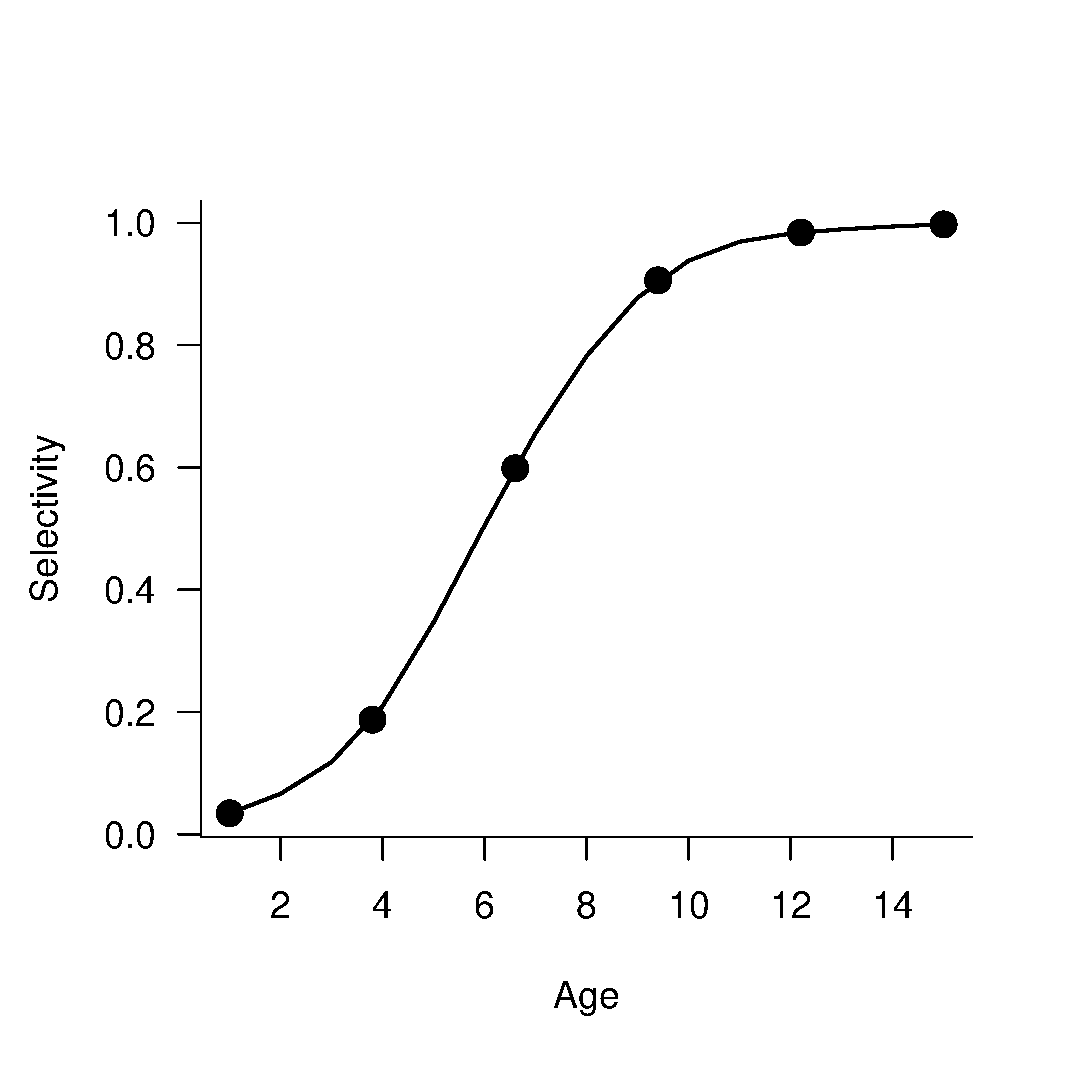
\includegraphics[width=\columnwidth]{iscamFigs/SplineEg.eps}\\
	\caption{Example of a natural cubic spline interpolation for estimating selectivity coefficients.  In \iscam\ the user specifies the number of nodes (circles) to estimate; then age-specific selectivity coefficients are interpolated using a natural cubic spline.}\label{Fig2}
\end{figurehere}

The same penalty functions for curvature and dome-shaped selectivity are also invoked for the cubic spline interpolation of selectivity.

\paragraph{Time-varying selectivity with cubic spline interpolation} A fourth option allows for cubic spline interpolation for age-specific selectivity  in each year.  This option adds a considerable number of estimated parameters but the most extreme flexibility.  For example, given 40 years of data and estimated 5 age nodes, this amounts 200 (40 years times 5 ages) estimated selectivity parameters.  Note that the only constraints at this time are the dome-shaped penalty and the curvature penalty; there is no constraint implemented for say a random walk (first difference) in age-specific selectivity).  As such this option should only be used in cases where age-composition data is available for every year of the assessment.

\paragraph{Bicubic spline to interpolate over time and ages}  The fifth option allows for a two-dimensional interpolation using a bicubic spline (Figure \ref{Fig3}).  In this case the user must specify the number of age and year nodes.  Again the same curvature and dome shaped constraints are implemented.  It is not necessary to have age-composition data each and every year as in the previous case, as the bicubic spline will interpolate between years.  However, it is not advisable to extrapolate selectivity back in time or forward in time where there are no age-composition data unless some additional constraint, such as a random-walk in age-specific selectivity coefficients is implemented (as of \today, this has not been implemented).

\begin{figure*}[!tbp]
	% Requires \usepackage{graphicx}
	\centering
	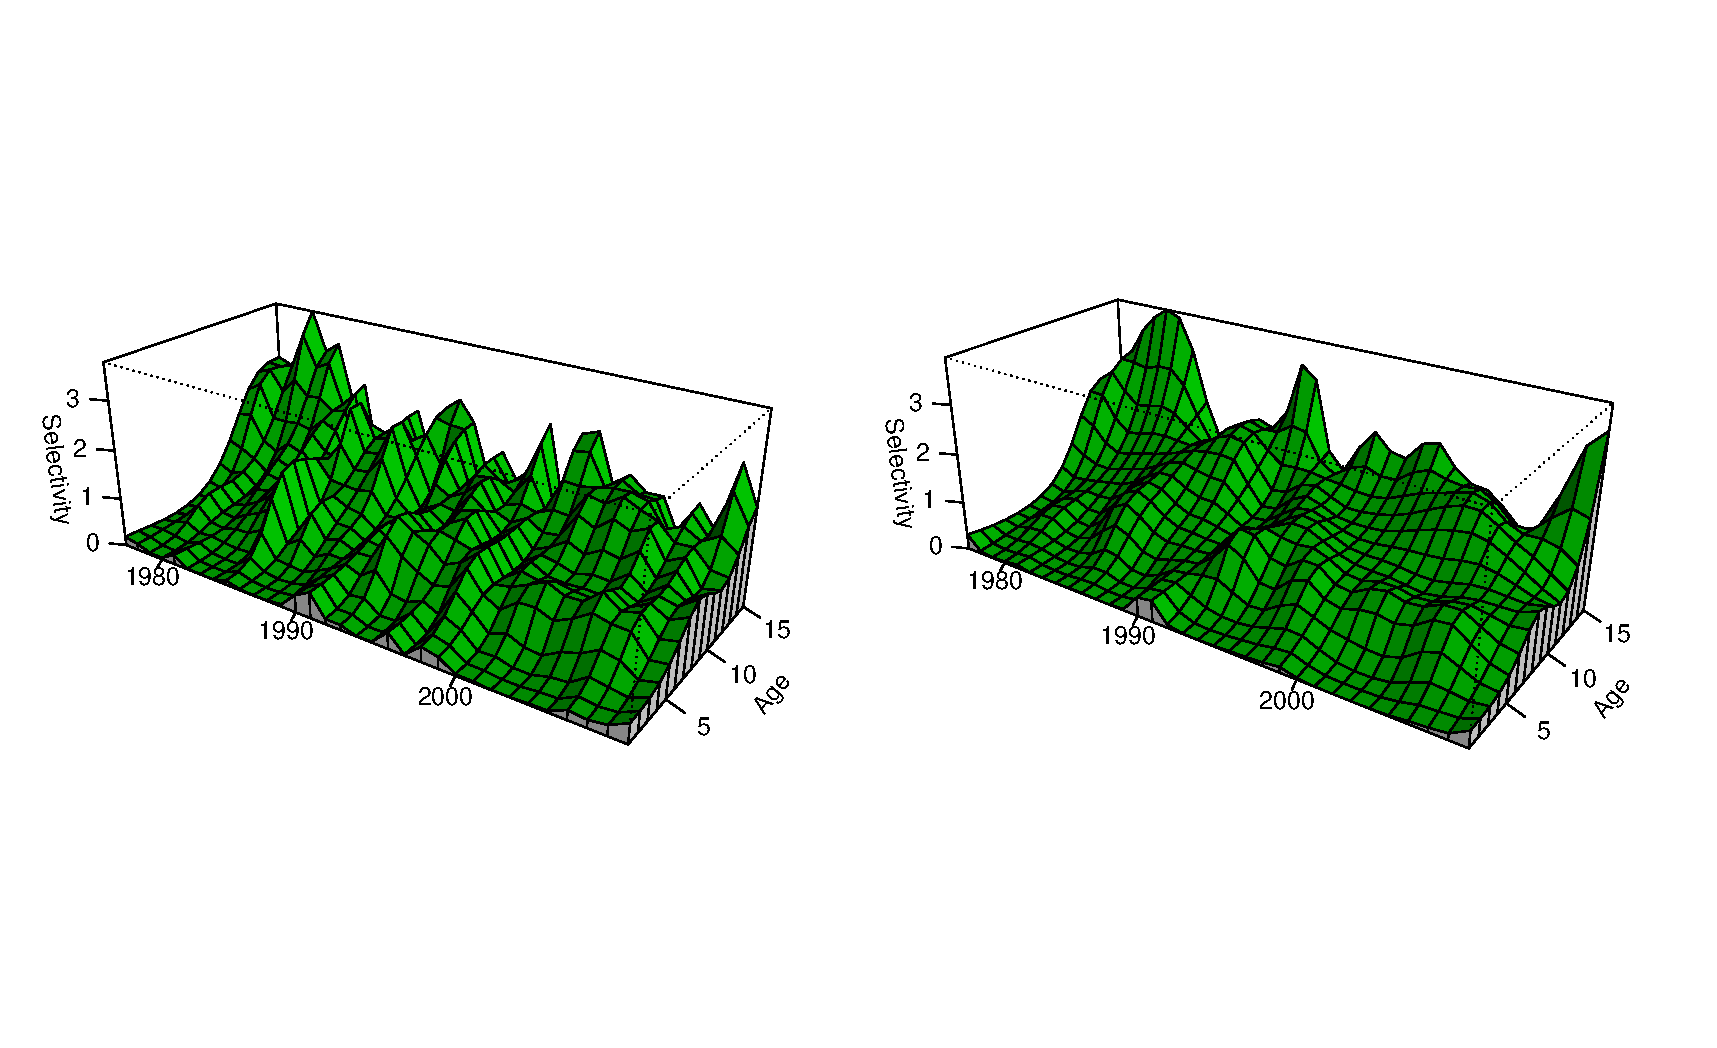
\includegraphics[width=0.9\textwidth]{iscamFigs/BicubicEg.eps}\\
	\caption{Example of a time-varying cubic spline (left) and bicubic spline (right) interpolation for selectivity as applied to the Pacific hake data. The panel on the left contains 165 estimated selectivity parameters and the bicubic interpolation estimates 85 selectivity parameters, or 5 age nodes and 17 year nodes. There are 495 actual nodes being interpolated.}\label{Fig3}
\end{figure*}
\end{multicols}

\subsection{Residuals, likelihoods \& objective function value components}
\begin{multicols}{2}
There are 3 major components to the overall objective function that are minimized while \iscam\ is performing maximum likelihood estimation.  These components consist of the likelihood of the data, prior distributions and penalty functions that are invoked to regularize the solution during intermediate phases of the non-linear parameter estimation.  This section discusses each of these in turn, starting first with the residuals between observed and predicted states followed by the negative loglikelihood that is minimized.

\subsubsection{Catch data}
It is assumed that the measurement errors in the catch observations are log-normally distributed, and the residuals is given by:
\begin{equation}\label{eq2}
\eta_{k,t}=\ln(C_{k,t}+o) -  \ln(\hat{C}_{k,t}+o),
\end{equation}
where $o$ is  a small constant (1.e-10) to ensure the residual is defined in the case of a 0 catch observation.  The residuals are assumed to be normally distributed with a user specified standard deviation $\sigma_{C}$.  At present, it is assumed that observed catches for each gear $k$ is assumed to have the same standard deviation.  To aid in parameter estimation, two separate standard deviations are specified in the control file: the first is the assumed standard deviation used in the first, second, to N-1 phases, and the second is the assumed standard deviation in the last phase.  The negative loglikelihood (ignoring the scaling constant) for the catch data is given by:
\begin{equation}\label{eq3}
\ell_C = \sum_k\left[  T_k\ln(\sigma_C)+\frac{\sum_t(\eta_{k,t})^2}{2\sigma_C^2}\right],
\end{equation}
where $T_k$ is the total number of catch observations for gear type $k$.


\subsubsection{Relative abundance data}
The relative abundance data are assumed to be proportional to biomass that is vulnerable to the sampling gear:
\begin{equation}\label{eq4}
 V_{k,t} = \sum_a N_{t,a} v_{k,a} w_a,
\end{equation}
where $v_{k,a}$ is the age-specific selectivity of gear $k$, and $w_a$ is the mean-weight-at-age.  For now, \iscam\ assumes that the index is measured at the start of each year before any significant mortality takes place.  The residuals between the observed and predicted relative abundance index is given by:
\begin{equation}\label{eq5}
\epsilon_{k,t} = \ln(I_{k,t}) - \ln(q_k)+\ln(V_{k,t}),
\end{equation}
where $I_{k,t}$ is the observed relative abundance index, $q_k$ is the catchability coefficient for index $k$, and $V_{k,t}$ is the predicted vulnerable biomass at the time of sampling.  The catchability coefficient $q_k$ is evaluated at its conditional maximum likelihood estimate:
\[
  q_k =\frac{1}{N_k} \sum_{t \in I_{k,t}} \ln(I_{k,t}) - \ln(V_{k,t}),
\]
where $N_k$ is the number of relative abundance observations for index $k$ \citep[see][for more information]{walters1994calculation}. The negative loglikelihood for relative abundance data is given by:
\begin{align}
\ell_I &= \sum_k \sum_{t \in I_{k,t}}  \ln(\sigma_{k,t})+\frac{\epsilon_{k,t}^2}{2\sigma_{k,t}^2} \label{eq6}\\
&\mbox{where}\nonumber\\
\sigma_{k,t} &= \frac{\rho \varphi^2}{ \omega_{k,t}},  \nonumber
\end{align}
where $\rho \varphi^2$ is the proportion of the total error that is associated with observation errors, and $\omega_{k,t}$ is a user specified relative weight for observation $t$ from gear $k$.  The $ \omega_{k,t}$ terms allow each observation to be weighted relative to the total error $\rho \varphi^2$; for example, to omit a particular observation, set $\omega_{k,t}=0$, or to give 2 times the weight, then set  $\omega_{k,t}=2.0$. To assume all observations have the same variance then simply set  $\omega_{k,t}=1$.  Note that if  $\omega_{k,t}=0$ then equation \eqref{eq6} is undefined; therefore, \iscam adds a small constant to  $\omega_{k,t}$ (1.e-10, which is equivalent to assuming an extremely large variance)  to ensure the likelihood can be evaluated.

\subsubsection{Age composition data}
Sampling theory suggest that age composition data are derived from a multinomial distribution \citep{fournier1982general}; however, \iscam\ assumes that age-proportions are obtained from a multivariate logistic distribution \citep{schnute1995influence}.  The main reason \iscam\ departs from the traditional multinomial model has to do with how the age-composition data are weighted in the objective function.  First, the multinomial distribution requires the specification of an effective sample size; this may be done arbitrarily or through iterative re-weighting \citep{MCALLISTER1997,gavaris2002sif}, and in the case of multiple and potentially conflicting age-proportions this procedure may fail to converge properly.  The assumed effective sample size can have a large impact on the overall model results.  

A nice feature of the multivariate logistic distribution is that the age-proportion data can be weighted based on the conditional maximum likelihood estimate of the variance in the age-proportions.  Therefore, the contribution of the age-composition data to the overall objective function is ``self-weighting'' and is conditional on other components in the model.

Ignoring the subscript for gear type for clarity, the observed and predicted proportions-at-age must satisfy the constraint 
\[
 \sum_{a=1}^A p_{t,a} = 1
\]
for each year. The residuals between the observed ($p_{t,a}$) and predicted proportions ($\widehat{p_{t,a}}$) is given by:
\begin{equation}\label{eq7}
\eta_{t,a}=\ln(p_{t,a})-\ln(\widehat{p_{t,a}})-\frac{1}{A}\sum_{a=1}^A\left[\ln(p_{t,a})-\ln(\widehat{p_{t,a}}) \right].
\end{equation}
The conditional maximum likelihood estimate of the variance is given by
\[
\widehat{\tau}^2=\frac{1}{(A-1)T}\sum_{t=1}^T\sum_{a=1}^A \eta_{t,a}^2,
\]
and the negative loglikelihood evaluated at the conditional maximum likelihood estimate of the variance is given by:
\begin{equation}\label{eq8}
	\ell_A = (A-1)T \ln(\widehat{\tau}^2).
\end{equation}
In short, the multivariate logistic likelihood for age-composition data is just the log of the residual variance weighted by the number observations over years and ages.

\subsubsection{Stock-recruitment}
There are two alternative stock-recruitment models available in \iscam: the Beverton-Holt model and the Ricker model.  Annual recruitment and the initial age-composition are treated as latent variables in \iscam, and residuals between estimated recruits and the deterministic stock-recruitment models are used to estimate unfished spawning stock biomass and recruitment compensation.  The residuals between the estimated and predicted recruits is given by
\begin{equation}\label{eq9}
	\delta_t = \ln(\bar{R}e^{w_t}) - f(B_{t-k})
\end{equation}
where $f(B_{t-k})$ is given by either \eqref{T4.12} or \eqref{T4.13}, and $k$ is the age at recruitment.  Note that a bias correction term for the lognormal process  errors is included in  \eqref{T4.12} and \eqref{T4.13}.

The negative log likelihood for the recruitment deviations is given by the normal density (ignoring the scaling constant):
\begin{equation}\label{eq10}
 \ell_\delta = n\ln(\tau) + \frac{\sum_{t=1+k}^T \delta^2_t}{2\tau^2}
\end{equation}
Equations \eqref{eq9} and \eqref{eq10} are key for estimating unfished spawning stock biomass and recruitment compensation via the recruitment models.  The relationship between ($s_o,\beta$) and ($B_o,\kappa$) is defined as:
\begin{align}
s_o &= \kappa/\phi_E\\
\beta&=\begin{cases}
\frac{\kappa-1}{B_o} \quad \mbox{Beverton-Holt}\\[1ex]
\frac{\ln(\kappa)}{B_o} \quad \mbox{Ricker}
\end{cases}
\end{align}
where $s_o$ is the maximum juvenile survival rate, and $\beta$ is the density effect on recruitment.


\end{multicols}

% \clearpage

    
    \section{Example Assessment: the Namibian hake case study}
\begin{multicols}{2}
As a simple example of fitting \iscam\ to CPUE data only, we use the Namibian hake case study from chapter 10 in the Ecological Detective \citep{hilborn1997ecological}.  In this example the available data consist of catch (thousands of tons) and CPUE (tons per standardized trawl hour).  \cite{hilborn1997ecological} provide three alternative models to the data that range from simple 4 parameter Schaefer production models (observation \& process error only) and a 5 parameter lagged recruitment, growth/survival model.  In this example they assume the stock is at an unfished state in 1967.

To conduct the assessment using \iscam\ with the same unfished assumption in 1965, the 			``Assume unfished in first year (0=FALSE, 1=TRUE)'' flag must be set to 1 (see the following control file). \iscam\ is an age-structured model, and in this example there are no available age-composition data to compare with. Therefore we must also assume a selectivity curve for this fishery.  In this example, selectivity was assume to follow a logistic function with the 50\% vulnerability-at-age equal to 3.5 years with a standard deviation of  1.0 years.  It is also necessary in this case to turn off the estimation of the selectivity parameters by setting the estimation phase to a negative number (e.g., -1).  

For the estimated leading parameters, two of the six parameters are not estimated \verb"#log_m" and \verb"#rho", which is the instantaneous natural mortality rate and the proportion of the total error that is associated with observation errors.  A bounded uniform prior is assumed for $R_o$ and a beta prior for steepness $h$ with an expected value of 0.6.  The natural mortality rate $M$ is assumed known and fixed at a value of 0.345.  A uniform bounded prior is assumed for the log of the average recruitment level, and a non-informative gamma prior is assumed for the total precision $\kappa$.  In this example we assume that the total error is allocated to observation and process error equally ($\rho= 0.5$).

\tiny
\noindent \hrulefill
\begin{alltt}
Control file for the Namibian hake data.
\input{../NamibianHake.ctl}
\end{alltt}
\hrulefill
\normalsize

To convert numbers-at-age to biomass, growth was based on the von Bertalanffy growth parameters in the \verb"NamibianHake.dat" file and the allometric relationship $w_a=a(l_a)^b$. Maturity-at-age is  based on the logistic function with age-4 being the age at 50\% maturity and 0.2 is the standard deviation. The plus group age was assumed to be 25 years, and there is only one fishing gear exploiting this stock.

Catch is taken by a single gear each year between 1965 and 1987, and the relative abundance index is based on the catch per standardized hour of trawling for the commercial gear.  It is assumed that each CPUE observation is assumed to have the same error distribution, and the relative weights of each observations are all set equal to one.

There is no age-composition data to speak of, but \verb"#na_gears" must have a value of 1 in order to proceed with reading the remaining portion of the data file.

\tiny
\noindent \hrulefill
\begin{alltt}
Control file for the Namibian hake data.
\input{../NamibianHake.dat}
\end{alltt}
\hrulefill
\normalsize

%%Results for Namibian hake.
\subsection{Maximum likelihood estimates of the model parameters}
Estimates of unfished spawning biomass is 2,877, steepness is 0.79, MSY is 266, and \fmsy is 0.33.  These results are  very similar to those obtained by \cite{hilborn1997ecological} for the Schaefer model with observation error.  Estimates of the total standard deviation amount to 0.16 which equally breaks down to 0.081 for observation and process errors.

\begin{figurehere}
	\centering
	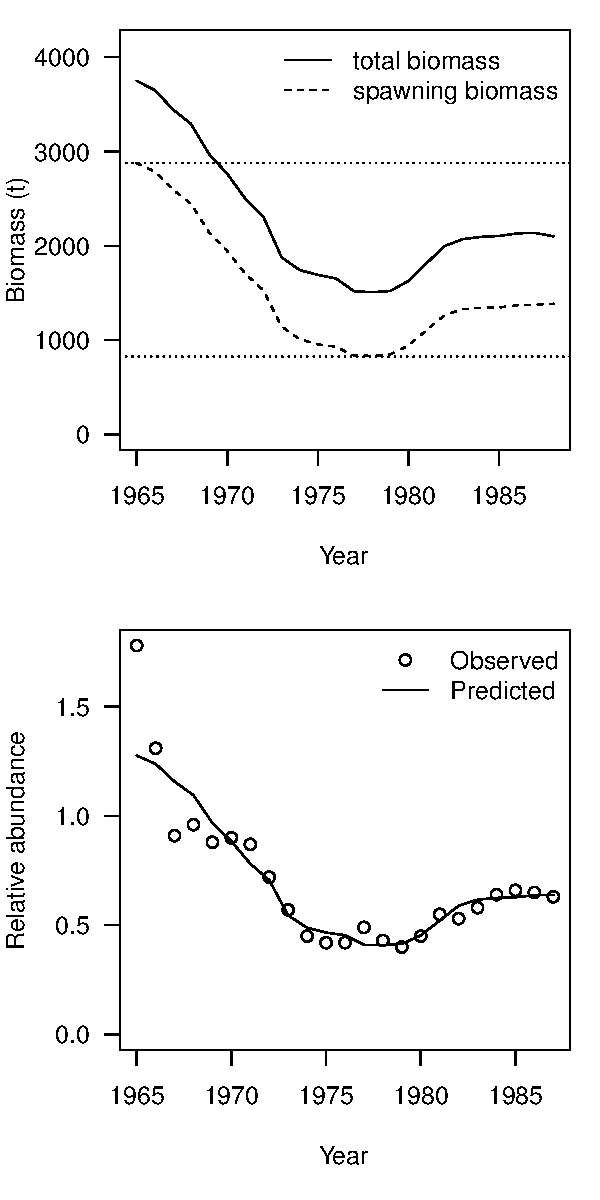
\includegraphics[width=\columnwidth]{iscamFigs/NhakeFigs.eps}
	\caption{Estimates of total biomass and spawning biomass, observed and predicted CPUE, for the Namibian hake data from \iscam. Unfished biomass, \bmsy, and MSY based depletion levels are shown as horizontal dotted lines.}\label{fig4}
\end{figurehere}

\subsection{Bayesian analysis of model parameters \& policy parameters}
Marginal posterior distributions of model parameters were constructed by using the metropolis algorithm built into ADMB to sample from the joint posterior distribution.  This is accomplished by running \iscam\ in -mcmc mode followed by the -mceval option to produce the \verb"iscam.mcmc" output file.  In this example an MCMC chain of length 1,000,000 was run and samples were taken systematically every 500 iterations (\verb"-mcsave 500"), which results in a posterior sample size of 2000.

Uniform prior distributions for the unfished recruitment and average recruitment ($R_0$ and $\bar{R}$), and non-informative gamma prior for the precision parameter ($1/\vartheta$).  In the case of the steepness parameter, a non-informative beta prior was used ($p(h)\sim beta[1.01,1.01]$), where steepness is re-scaled to the interval 0.2-1.0 (i.e, $(h-0.2)/0.8$) such that a 0 probability was assigned for $h$ values less than 0.2.  In comparison to the results obtained by \cite{hilborn1997ecological} using a biomass production model with lagged recruitment and a Beverton-Holt recruitment function, the data here appear to have some information about the steepness parameter (Fig. \ref{fig5}).  This owes in part to differences in assumptions about growth, maturity and selectivity between the LRGS model used by \cite{hilborn1997ecological} and this \iscam\ example.

\begin{figurehere}
	% Requires \usepackage{graphicx}
	\centering
	\psfrag{log.ro}[c][][0.75]{$\ln(R_0)$}
	\psfrag{log.rbar}[c][][0.75]{$\ln(\bar{R})$}
	\psfrag{kappa}[c][][0.75]{$\vartheta$}
	\psfrag{h}[c][][0.75]{$h$}
	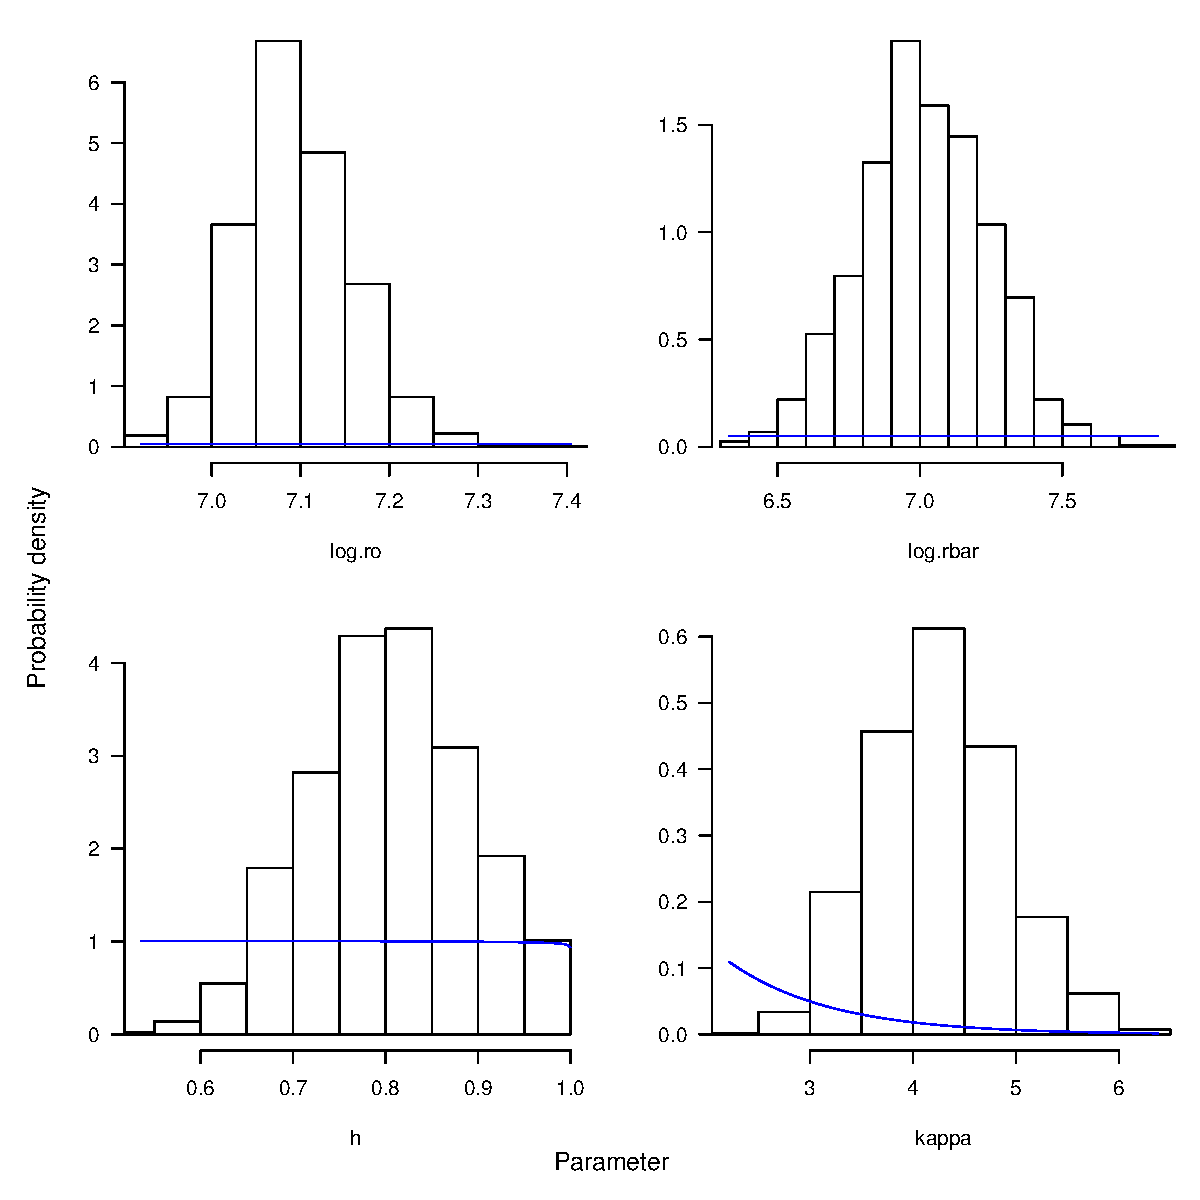
\includegraphics[width=\columnwidth]{iscamFigs/fig5.eps}\\
	\caption{Marginal posterior probability densities (histograms) and prior densities (lines) for unfished recruitment $R_0$, steepness $h$, mean recruitment $\bar{R}$ and recruitment compensation $\kappa$ for the Namibian hake case study.}\label{fig5}
\end{figurehere}

Marginal posterior densities can also be produced for derived quantities such as MSY based reference points (Fig \ref{fig6}).   Again, although not directly comparable due to structural differences between \iscam\ and the LRGS model, the marginal posterior distributions for MSY and $B_0$ are very similar.  More importantly however is that these marginal distributions can also be used to calculate the probability that the stock is currently overfished and if overfishing is occurring.  This is normally represented from a maximum likelihood perspective where the trends in biomass relative to \bmsy and fishing mortality rates relative to \fmsy are plotted against each other (these are known as KOBE plots, Fig \ref{fig7}).

\begin{figurehere}
	% Requires \usepackage{graphicx}
	\centering
	\psfrag{bo}[c][][0.75]{$B_0$}
	\psfrag{bmsy}[c][][0.75]{\bmsy}
	\psfrag{msy}[c][][0.75]{MSY}
	\psfrag{fmsy}[c][][0.75]{\fmsy}
	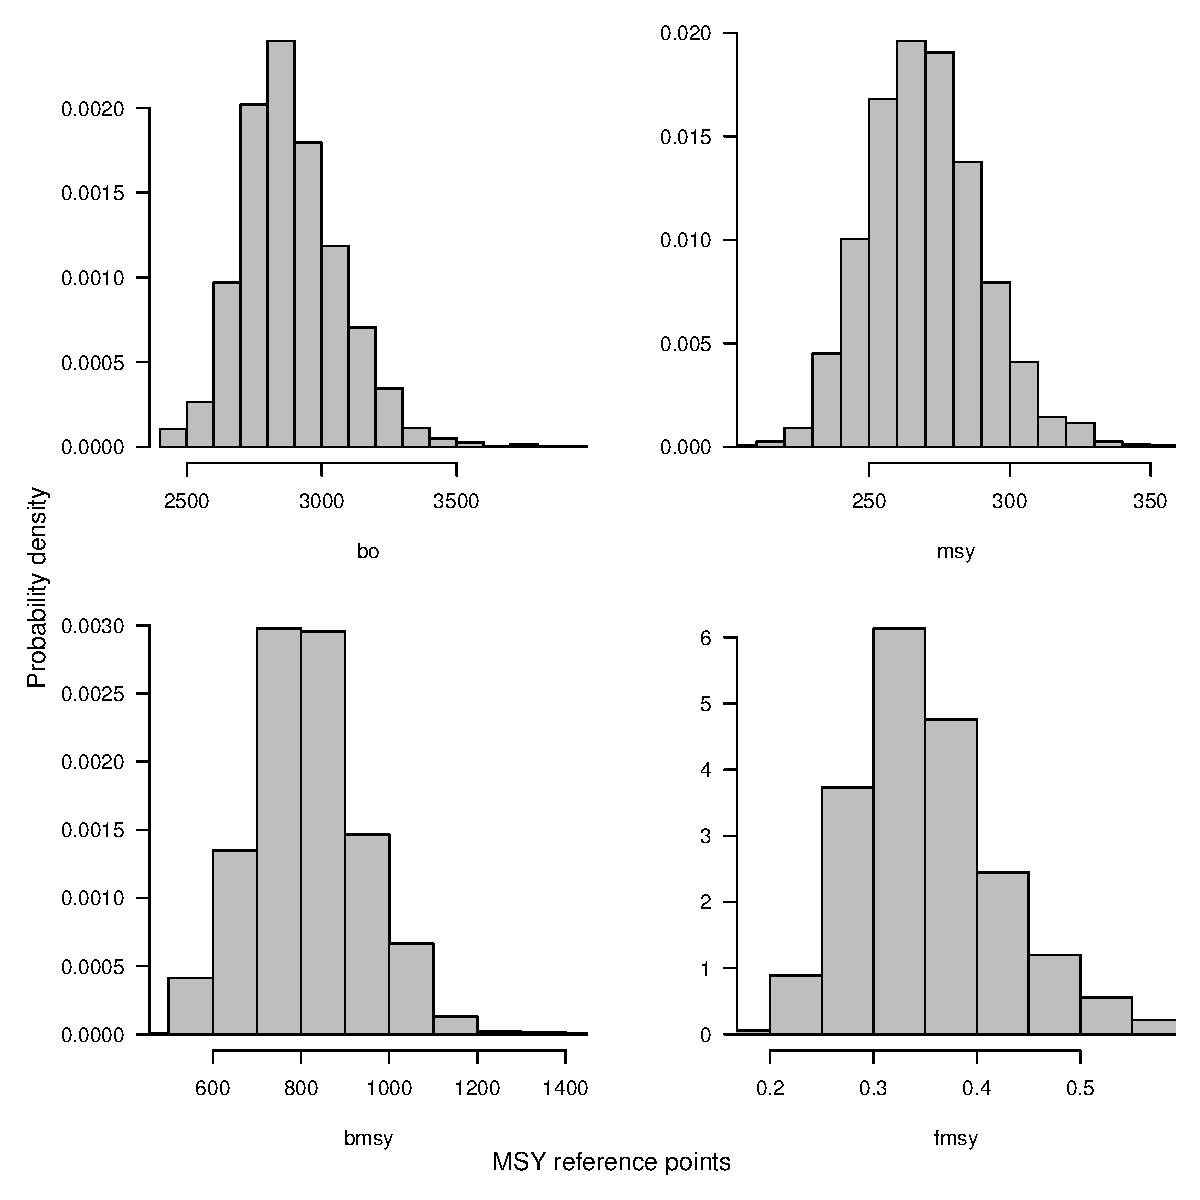
\includegraphics[width=\columnwidth]{iscamFigs/fig6.eps}\\
	\caption{Marginal posterior probability densities for unfished spawning biomass $B_0$, optimal spawning biomass \bmsy, MSY and \fmsy\ for the Namibian hake case study.}\label{fig6}
\end{figurehere}

\begin{figurehere}
	\centering
	\psfrag{bstatus}[c][][0.75]{$B_t/$\bmsy}
	\psfrag{fstatus}[c][][0.75]{$F_t/$\fmsy}
	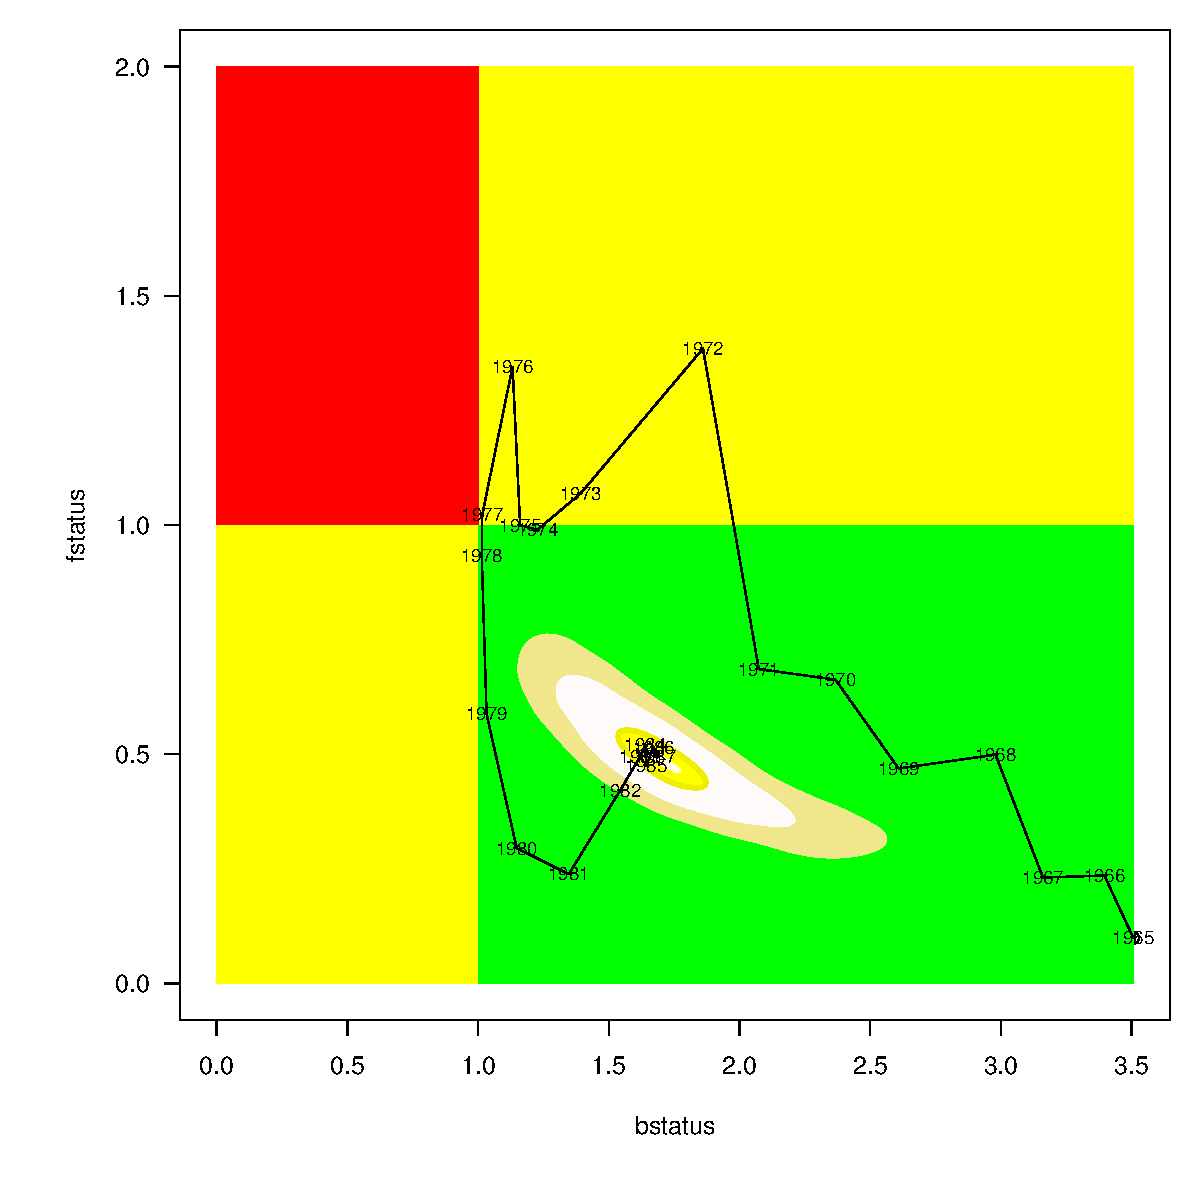
\includegraphics[width=\columnwidth]{iscamFigs/fig7.eps}\\
	\caption{Stock status plot (or Kobe plot) where the ``fried egg'' represents uncertainty.}\label{fig7}
\end{figurehere}

\end{multicols}



%%%%%%%%%%%%%%%%%%%%%%%%%%%%%%%%%%%%%%%%%%%%%%%%%%%%
%%%%%%%%%%%%%%%%%%%%%%%%%%%%%%%%%%%%%%%%%%%%%%%%%%%%
%%%%%%%%%%%%%%%%%%%%%%%%%%%%%%%%%%%%%%%%%%%%%%%%%%%%
\section{Example Assessment: the Pacific hake fishery}
\begin{multicols}{2}
\subsection{Data \& assumptions}
As more complex example assessment, the data from the Pacific hake fishery is used.  Pacific hake (\textit{Merluccius productus})  in the Northeast Pacific has a migratory coastal stock that is harvested by US and Canadian fishing fleets during the summer and late fall.  This data is an extension to the previous work in \cite{Martell2008pam}.  In this example the data has been restricted to the years 1977-2009, as this was a period when catch-age data from both the Canadian and US fisheries was available and could be aggregated using a weighted average based on the catch proportion from each nation.

The data from this fishery consists of a combined total catch, a relative abundance index from an acoustic survey conducted on a triannual and biannual basis, age-composition data from the commercial fishery, and finally age-composition data from the acoustic trawl survey. The coastal Pacific hake stock undergo an annual migration from spawning grounds in the south near Baja California Sur in the winter to summer feeding grounds to the north; the extent of the northward migration is highly variable and ranges from Oregon--Washington to Southeast Alaska in some years.  Larger/older fish tend to migrate further north.  Inter-annual variation in the extent of the migration leads to variation in selectivity to the fishery.  To accommodate the time-varying selectivity, a total of 85 nodes for a bicubic spline are estimated (17 nodes for the year effect, and 5 nodes for the age effect, see Fig. \ref{Fig3}).

In this example it was assumed that recruitment follows a Beverton-Holt relationship, the stock is not at its unfished state in 1977, natural mortality is independent of age and constant over time, and survey selectivity is asymptotic and time-invariant.  


Here is the \iscam\ control file for the Pacific hake data, and the data file is provided at the end of this section on page \pageref{HakeDataFile}.  The observed combined landings from both the US and Canadian zones have averaged about 233,000 metric tons between 1977 and 2009, and in the last 10 years has averaged 270,000 mt with a peak in 1994 of 361,000 mt  (Fig. \ref{fig8}.)\\
\tiny
\noindent \hrulefill
\begin{alltt}
\input{../PHake2010.ctl}
\end{alltt}
\hrulefill
\normalsize

\begin{figurehere}
	\centering
	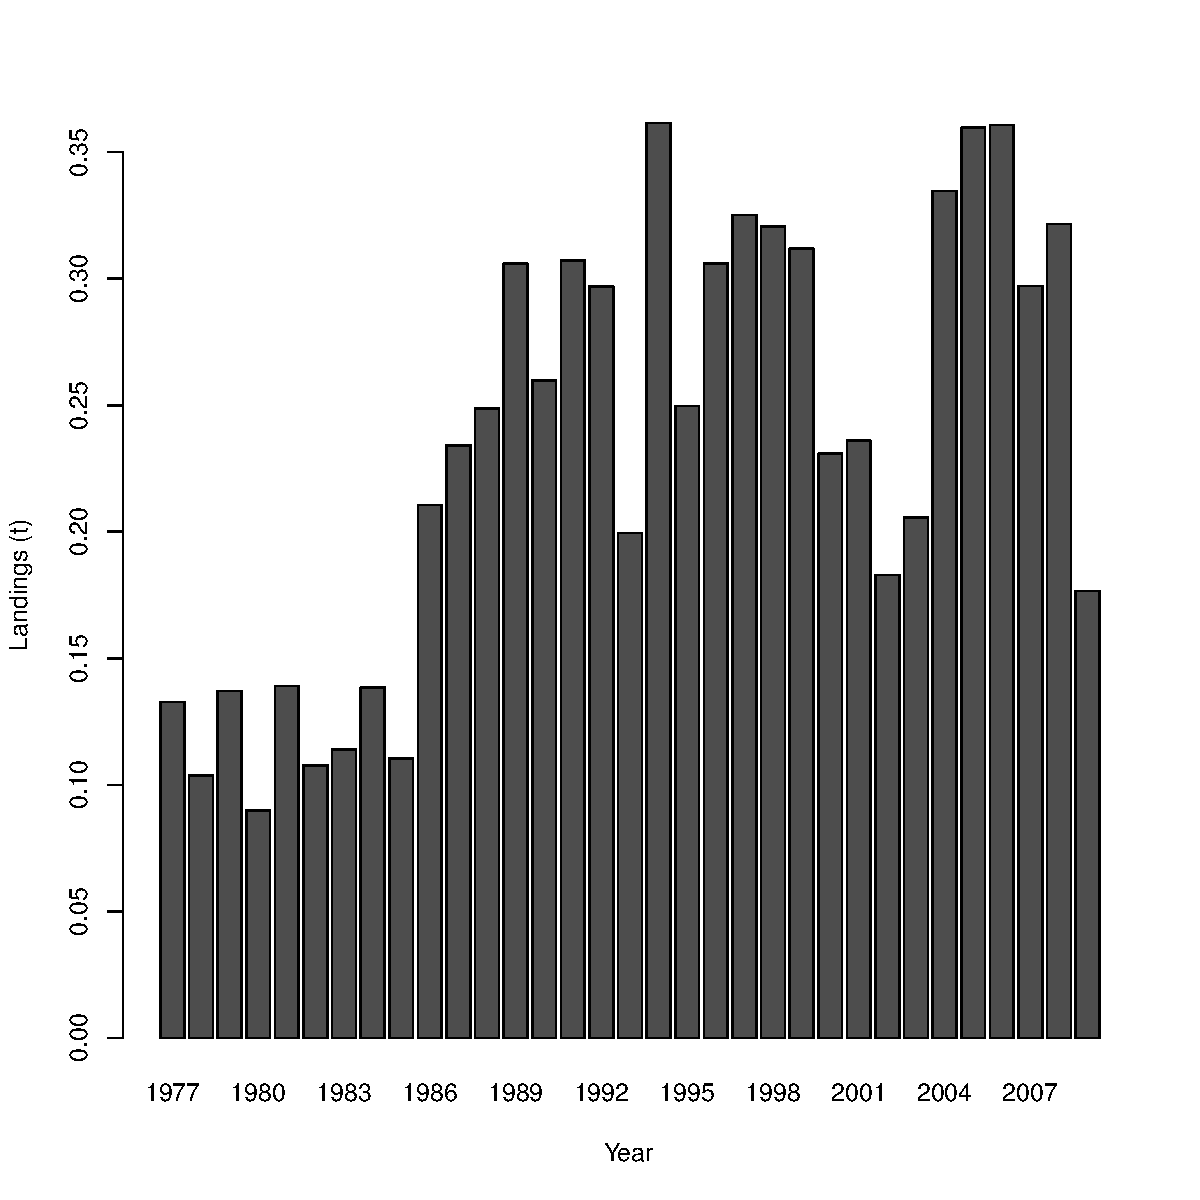
\includegraphics[width=0.8\columnwidth]{iscamFigs/phakefig15.eps}\\
	\caption{Combined observed landing from the US and CAN fisheries for Pacific hake between 1977 and 2009.}\label{fig8}
\end{figurehere}
%
%\begin{figurehere}
%	\centering
%	\includegraphics[width=0.4\columnwidth]{iscamFigs/phakefig1.eps}\\
%	\caption{Assumed age-schedule information for this example assessment.}\label{fig8b}
%\end{figurehere}


\subsection{Maximum likelihood estimates}
A total of 176 model parameters were estimated and it took  roughly 10 seconds to obtain maximum likelihood estimates, including the calculations for the Hessian matrix on a MacBook Pro, with a 2.66 GHz Intel Core i7 processor.

Maximum likelihood estimates of total biomass and spawning biomass along with estimates of $B_0$ and \bmsy are shown in Fig. \ref{fig9}.  Starting in 1977, estimates of spawning biomass was just slightly less than the estimate of \bmsy.  Starting in the 1980's, spawning biomass increased to a maximum in 1990 owing to two very large year classes (1980 and 1984, Fig. \ref{fig10}). Between 1985 and 1999, recruitment ranged between average and median values and the spawning stock biomass declined to less than \bmsy values in 2001 while fisheries removals exceeded 200,000 mt per year.  Another significant year class (1999) was responsible for rebuilding the spawning stock biomass up to 2004, and since 2005, the spawning stock biomass has continued to decline.

\begin{figurehere}
	\centering
	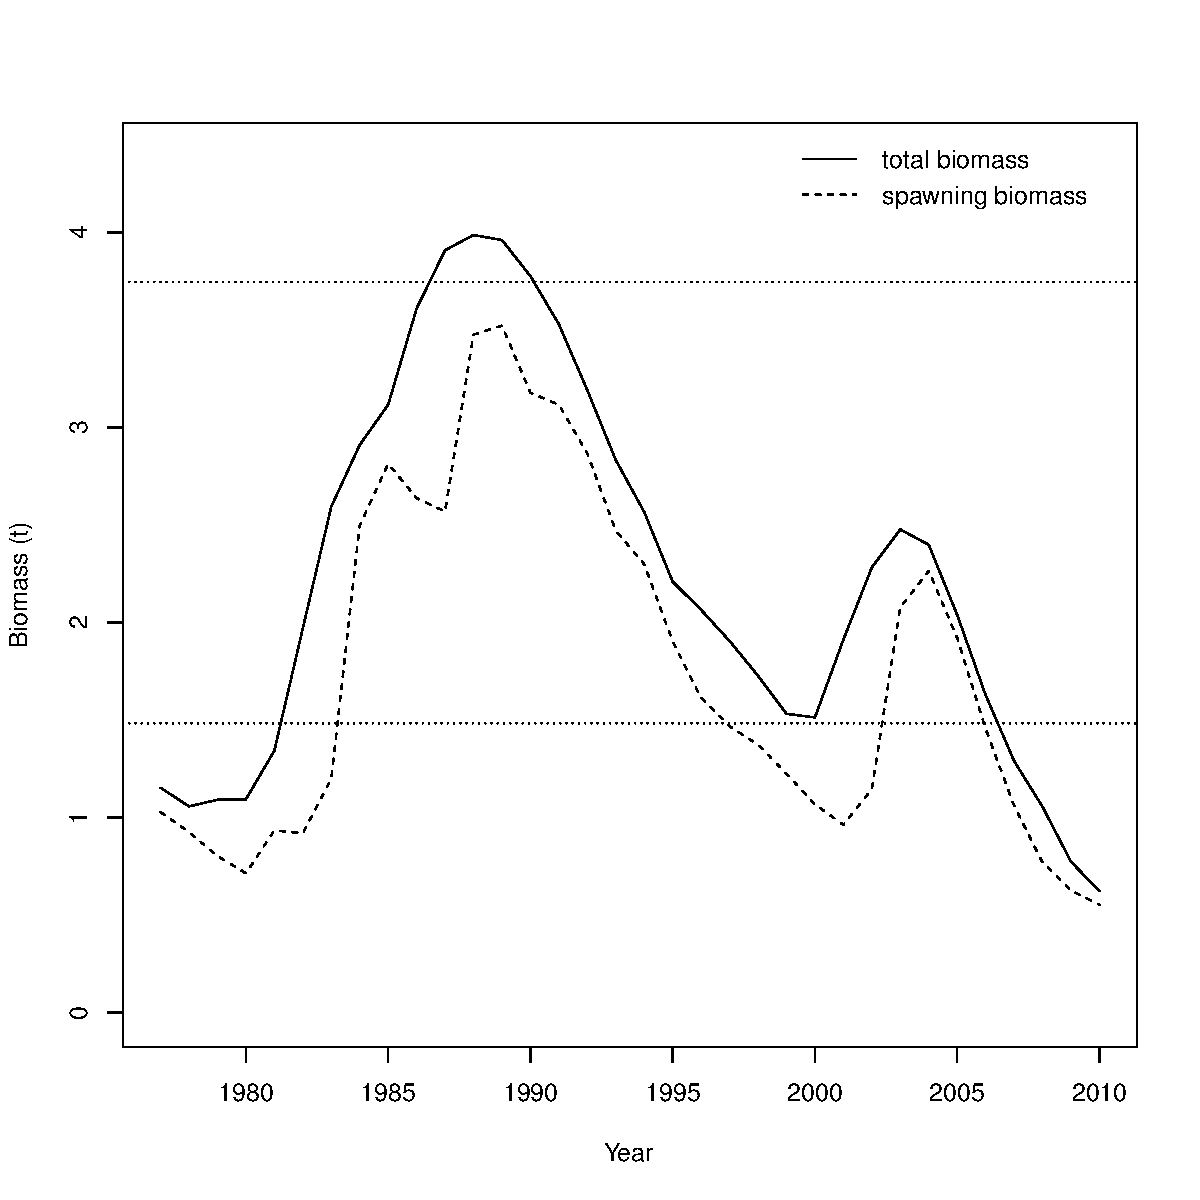
\includegraphics[width=0.95\columnwidth]{iscamFigs/phakefig2.eps}\\
	\caption{Maximum likelihood estimates of total biomass and spawning stock biomass for Pacific hake along with reference points (dotted lines) for unfished spawning biomass $B_0$ and \bmsy.}\label{fig9}
\end{figurehere}

Information to estimate age-1 recruitment for Pacific hake comes from the catch-age composition data.  Between 1978 and 2009 the average age-1 recruitment is estimated to be 2.72 billion individuals and the median value is 1.16 billion individuals (Fig. \ref{fig11}).  The maximum likelihood estimate of the standard deviation in recruitment ($\tau$, see eq. \ref{T4.2} on page \pageref{Table4}) was 1.29 given the prior information specified in the control file for this assessment.

\begin{figurehere}
	\centering
	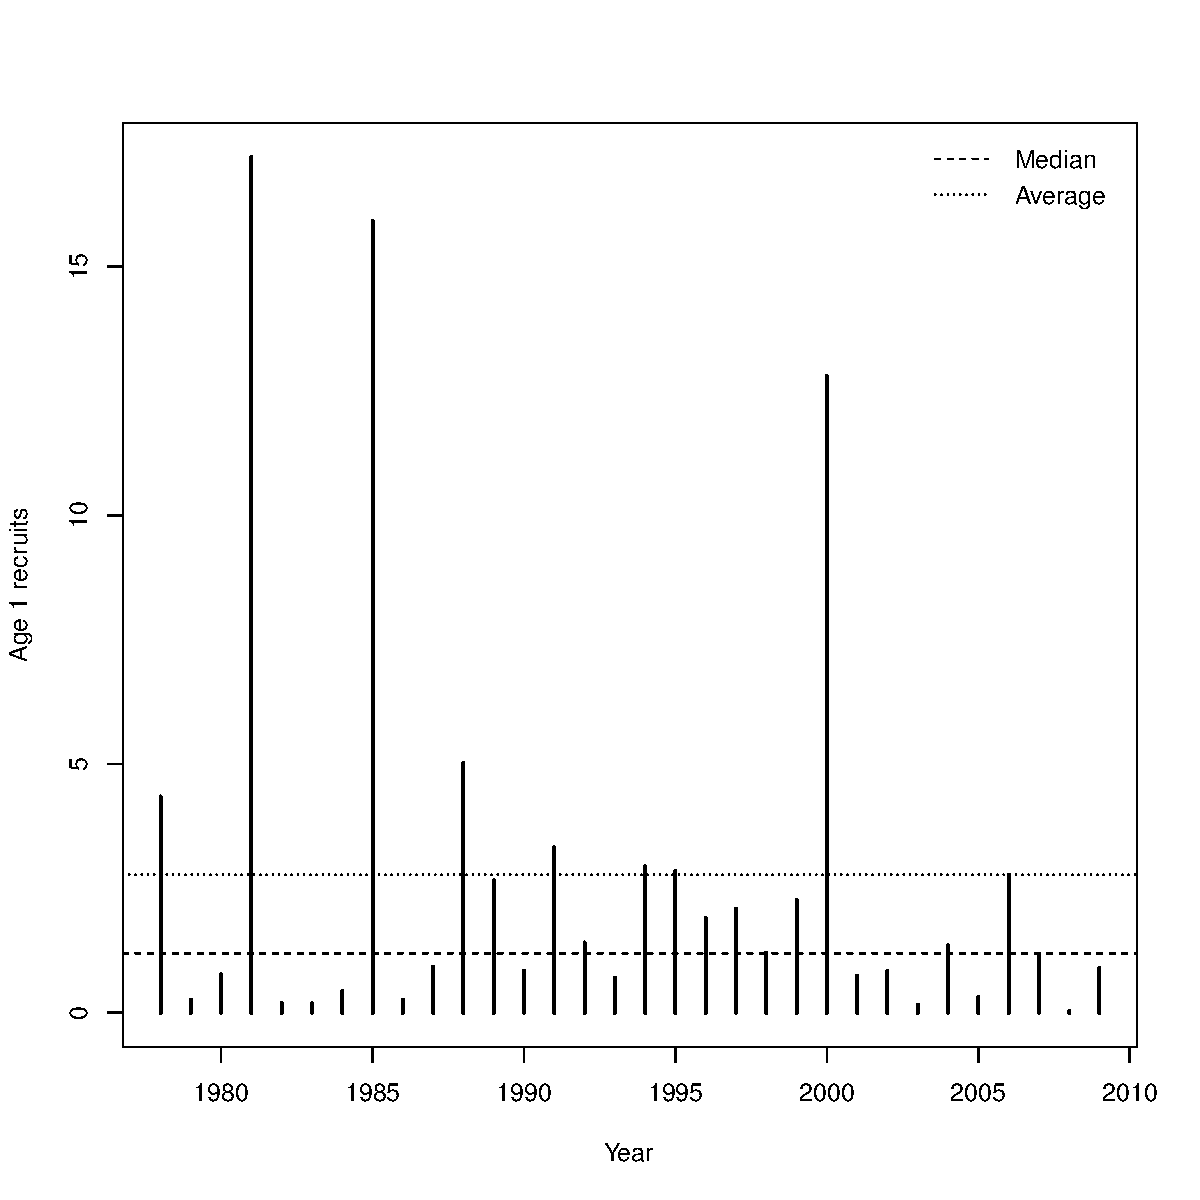
\includegraphics[width=0.95\columnwidth]{iscamFigs/phakefig14.eps}\\
	\caption{Maximum likelihood estimates of age-1 recruits from 1978 to 2009, with median and average values shown as the horizontal dashed and dotted lines.}\label{fig10}
\end{figurehere}

Current estimates of stock status relative to \bmsy\ and the removal rate relative to \fmsy is estimated to be in the critical zone in term of the Department of Fisheries and Oceans Canada, Fisheries Management Framework (Fig. \ref{fig11}).  Estimates of the spawning stock biomass are less than 80\% of \bmsy and are currently in the cautious zone.  Estimates of fishing mortality rate are roughly 1.5 times the estimate of \fmsy.  Maximum likelihood estimates of \bmsy and \fmsy are 1.13 million mt 0.336, respectively. 

\begin{figurehere}
	\centering
	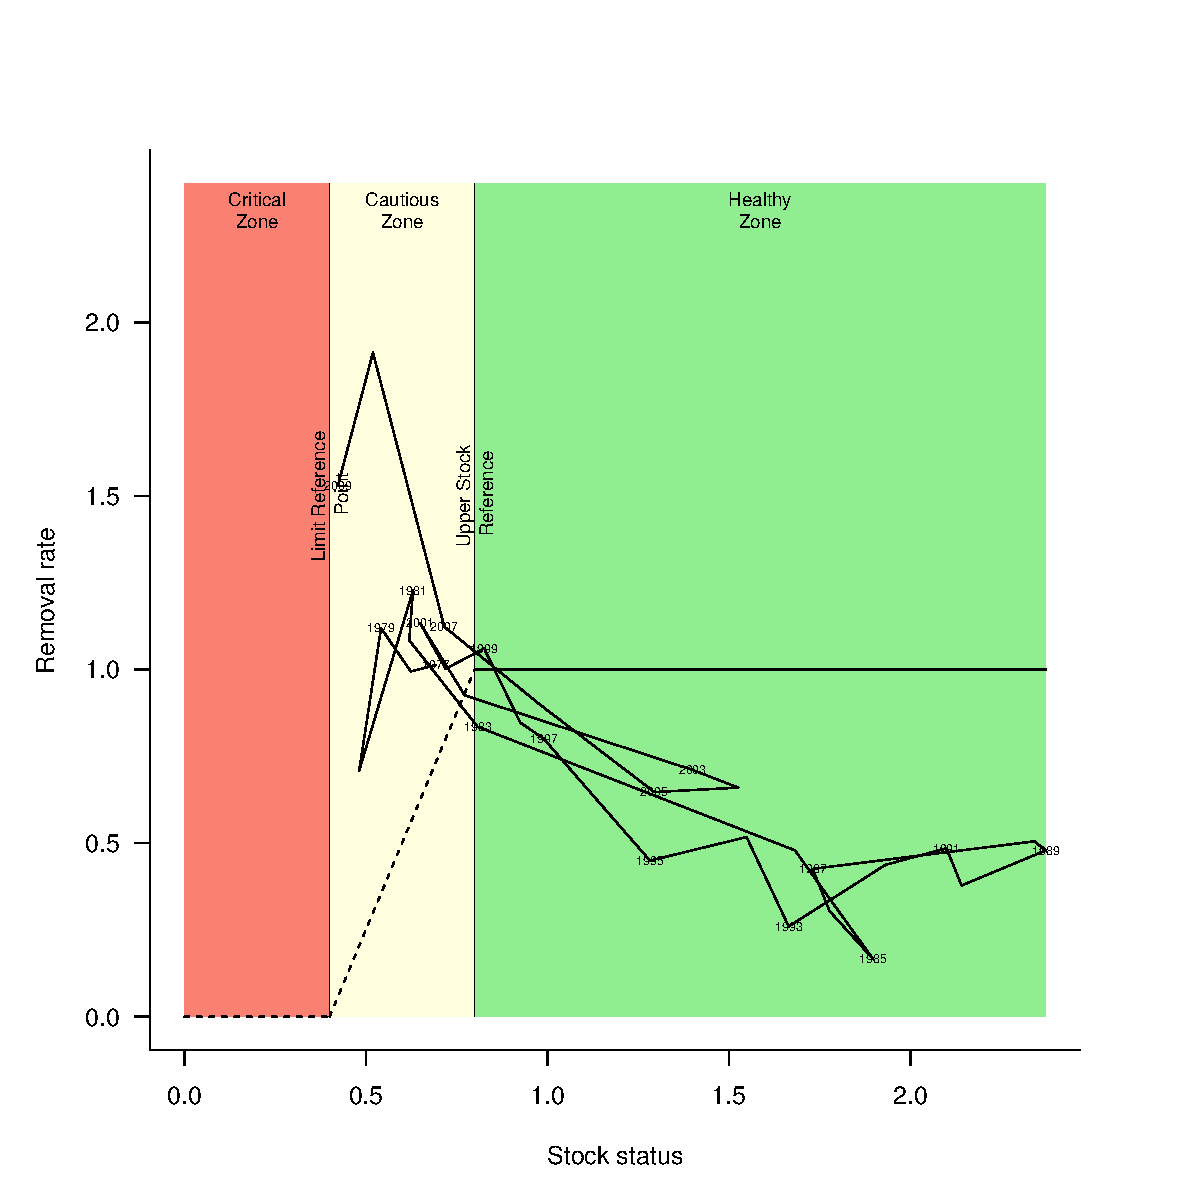
\includegraphics[width=0.95\columnwidth]{iscamFigs/phakefig8.eps}\\
	\caption{Maximum likelihood estimates of stock status ($B_t/$\bmsy) and removal rate ($F_t/$\fmsy) for Pacific hake relative to the Department of Fisheries and Oceans Canada's  Fisheries Management Framework.}\label{fig11}
\end{figurehere}

Model fit can be partially judged by the residual patterns between the observed and predicted data (Fig. \ref{fig12}).  The catch data are assumed to be measured fairly accurately with a small standard deviation ($\sigma_C=0.025$) in measurement errors; the largest residual in the catch is just less than 100 mt in 1981.  

Recall that \iscam\ directly estimates annual recruitment values, and the reported residuals in Fig. \ref{fig12} correspond to the log differences between the estimated recruitment and a Beverton-Holt model prediction where $R_0$ and steepness $h$ are the estimated parameters for the stock recruitment model.  The strong 1980, 1984 and 1999 cohorts, show up as strong positive residuals in 1981, 1985 and 2000 in the residual plot (note that the age-at-recruitment is 1 year).  The 2002 and 2004 cohorts appear to be well below the median values in recent years, and the 2005 cohort is currently estimated to be the next largest cohort since 1999.

\begin{figurehere}
	\centering
	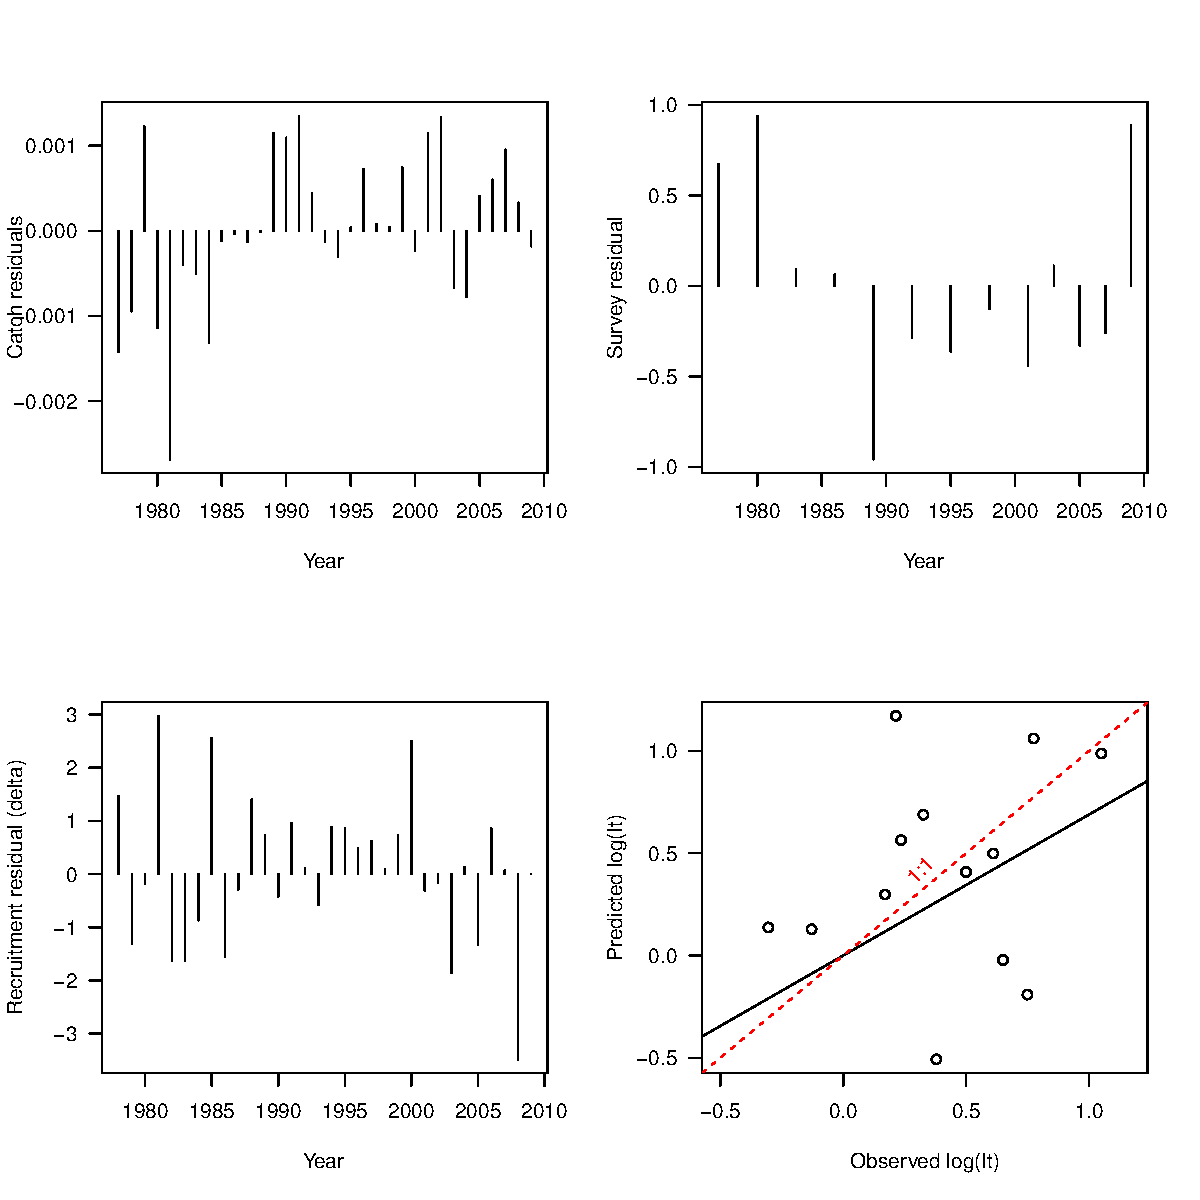
\includegraphics[width=0.95\columnwidth]{iscamFigs/phakefig11.eps}\\
	\caption{Residuals between the observed and predicted catch, deviations between estimated recruitment and a deterministic Beverton-Holt model, and the observed and predicted relative abundance data from the acoustic survey.}\label{fig12}
\end{figurehere}


\subsection{Time-varying selectivity}
Estimates of time-varying selectivity for the commercial fishery were based on estimating 85 nodes (17 years and 5 ages) and interpolating between these nodes using a bicubic spline.  The estimated nodes in \iscam\ are equidistant, and the total number of estimated nodes is specified in the control file.  Increasing the number of estimated nodes should improve the overall fit to the age-composition data; however, this comes at the expense of increasing the associated uncertainty in overall model parameter estimates.  To ensure that the model is not over-fitting the data, there are two additional penalties that are added to the objective function that limit the rate of change in age-effects (penalty weight for second differences), and how much dome-shaped is allowed in the age-effects.  Increasing the penalty weight on second differences insures a smoothed increase or decrease in the selectivity-at-age, and increasing the weight on the dome-shaped penalty reduces the amount of dome-shaped selectivity that can occur.  Again, these penalty weights are specified in the control file  in the selectivity parameters section.

In the Pacific hake example, estimates of selectivity increase with age during the late 1970s and early 1980s (Fig. \ref{fig13}).  As the 1980 and 1984 cohorts recruit to the fishery, the selectivity shifts to younger ages, and becomes more dome-shaped.  At the peak of the spawning stock biomass in 1990, selectivity increases continuously with age, and is more or less asymptotic until the 1999 cohort enters the fishery.  Recent estimates of selectivity indicate that the 1999 cohort (age-10 in the year 2009) is still strongly selected for, but as the biomass of the 1999 cohort erodes there is an apparent increase in selectivity for older ages (Fig. \ref{fig13}).

\begin{figurehere}
	\centering
	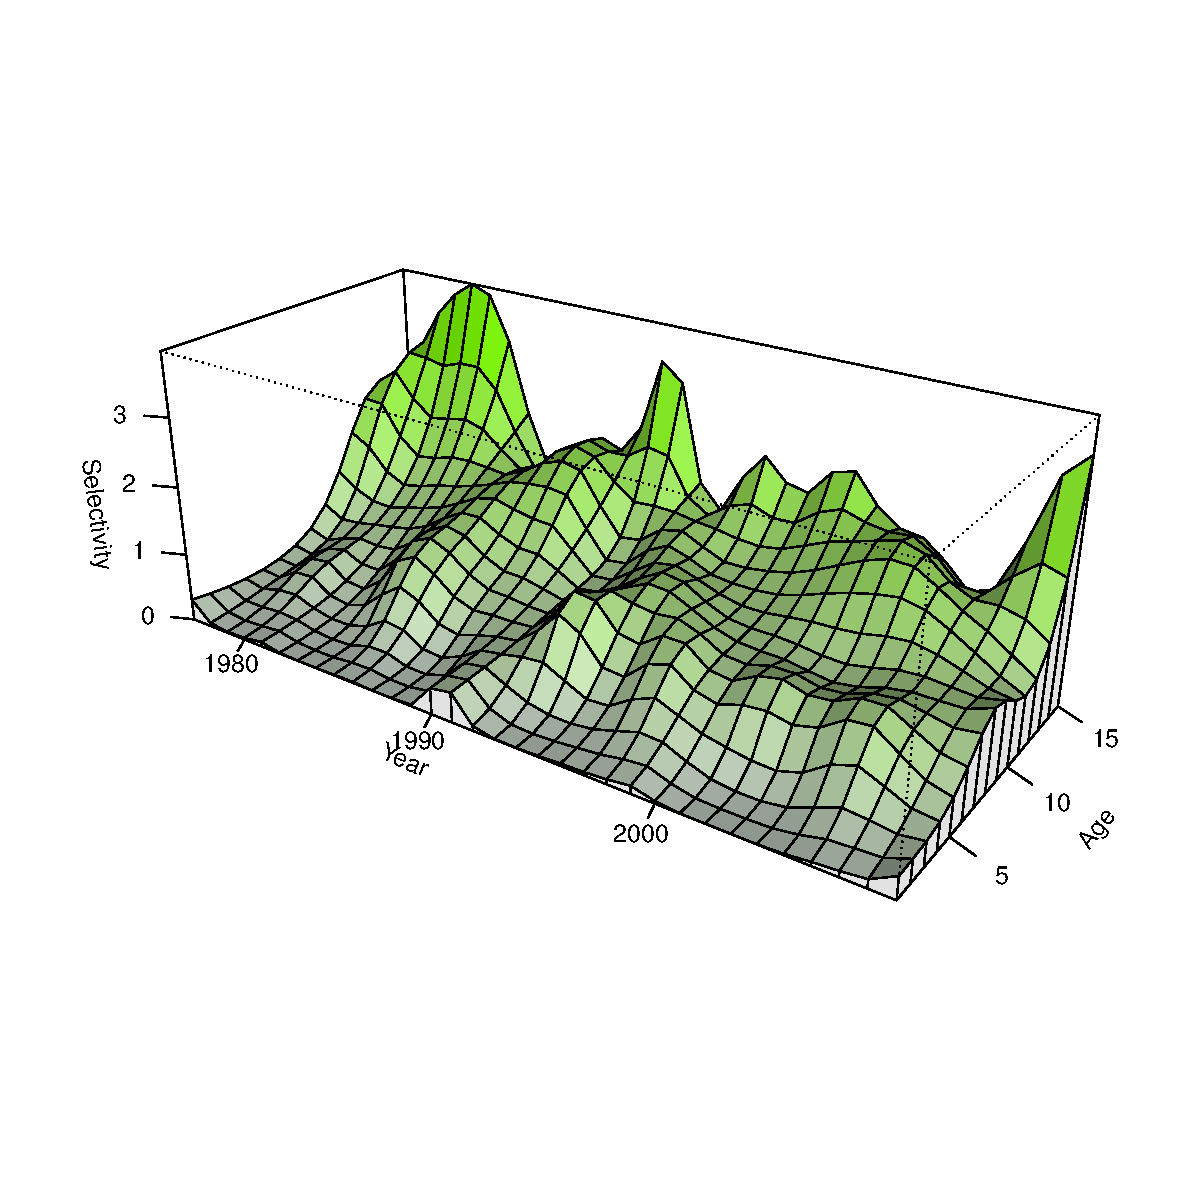
\includegraphics[width=\columnwidth]{iscamFigs/phakefig9a.eps}\\
	\caption{Estimates of selectivity for the commercial fishery.}\label{fig13}
\end{figurehere}

The residual patterns in the age composition data from the commercial fishery don't appear to have any significant pattern that would indicate a major model mis-specification (Fig. \ref{fig13a}).  There is a tendency for age-2 proportions to have more negative residuals and age-3 positive residuals, but over all these residuals are fairly small.  This is not much of a surprise given the flexibility of the time-varying selectivity that was assumed in the commercial fishery.

\begin{figurehere}
	\centering
	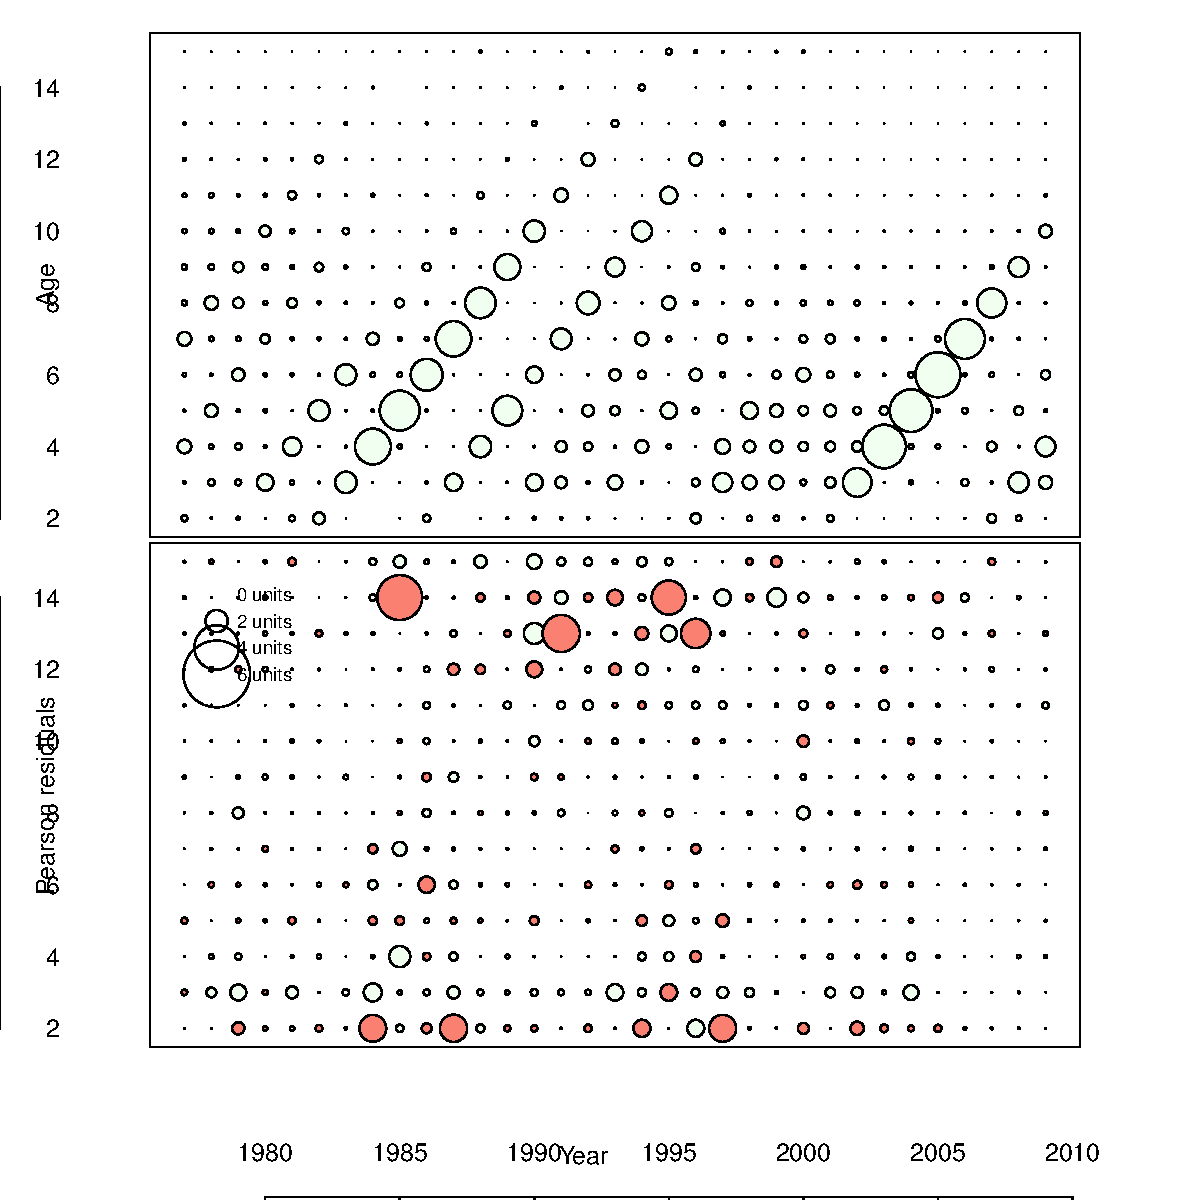
\includegraphics[width=\columnwidth]{iscamFigs/phakefig13a.eps}\\
	\caption{Observed age-composition (top panel) and Pearson residuals between observed and predicted proportions-at-age in the commercial fishery (bottom panel, with negative residuals given by dark circles).}\label{fig13a}
\end{figurehere}

Although not shown here, the residual pattern for the survey age composition also appears to be random, and in this case a time-invariant asymptotic selectivity curve was used for the acoustic survey. Survey data from 1995 to 2007 were assumed to be twice as accurate in comparison to the data collected prior to 1995 when spatial coverage of the survey was incomplete.  Also, the 2009 survey carries no weight as this survey was contaminated by the presence of Humboldt squid (\textit{Dosidicus gigas}) during the 2009 survey.  Additional details about the data for the Pacific hake assessment and the methods used to aggregate the age-composition for the US and CAN fisheries can be found in \cite{Martell2009}.

\subsection{Bayesian implementation}
To obtain samples from the joint posterior distribution and obtain median values and credible intervals, \iscam\ was run using the Metropolis-Hastings routine that is built into ADMB.  In this example, 2000 systematic samples from a chain of length 1,000,000 was used.  The total runtime for conducting a MCMC sample  of length 1,000,000 was 39 minutes and 56 seconds with 176 estimated parameters.

The marginal posterior distributions and the corresponding prior distributions are shown in Fig. \ref{fig14}.  There is no information in the data about the underlying steepness of the stock recruitment relationship; this is clearly shown by the marginal posterior distribution for $h$ reflects the assumed (\emph{ad hoc}) prior distribution.

\begin{figurehere}
	\centering
	\psfrag{log.ro}[c][][0.5]{$\ln(R_0)$}
	\psfrag{log.rbar}[c][][0.5]{$\ln(\bar{R})$}
	\psfrag{h}[c][][0.5]{$h$}
	\psfrag{rho}[c][][0.5]{$\rho$}
	\psfrag{log.m}[c][][0.5]{$\ln(M)$}
	\psfrag{kappa}[c][][0.5]{$\vartheta$}
	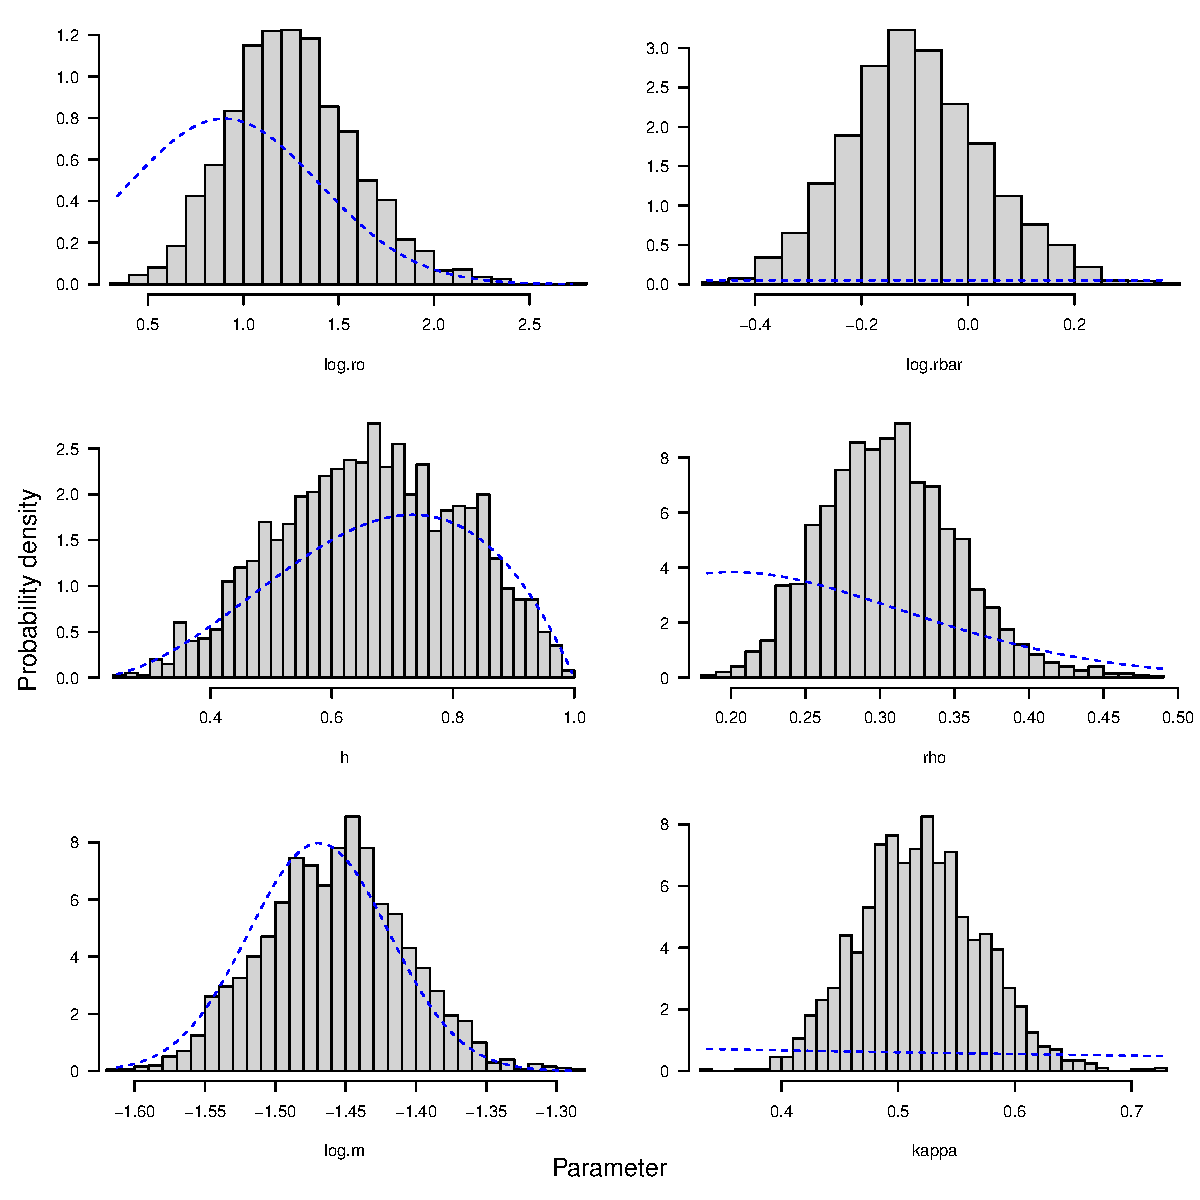
\includegraphics[width=\columnwidth]{iscamFigs/phakefig5.eps}\\
	\caption{Marginal posterior densities and prior densities for the leading parameters in \iscam.}\label{fig14}
\end{figurehere}

The prior distributions for each of the estimated leading parameters are specified in the control file.  In this example, a normal prior was assumed for the unfished recruitment ($\ln(R_0)$) and the log of the natural mortality rate ($\ln(M)$), a beta prior for the steepness ($h$) and the fraction of the total error that is associated with observation error ($\rho$), and a non-informative gamma prior for the total precision ($\vartheta$).  A uniform prior was specified for the average recruitment ($\ln(\bar{R})$).

Recent trends in the spawning stock biomass, and depletion, along with the associated uncertainty in the form of a credible interval are given in Table \ref{iscam.T1}.  Projected estimates of spawning stock depletion at the start of 2010 is 22\%, with a lower bound of 7.5\% and an upper bound of 53.2\%.  This translates into a projected spawning stock biomass of 670,000 mt with a 95\% credible interval of 255,000 mt to 1,506,000 mt.

\begin{tiny}
% latex.default(tail(t1, 10), file = filename, rowname = NULL,      caption = cap, cgroup = cgrp, n.cgroup = ncgrp, label = "iscam.T1") 
%
\begin{table}[!tbp]
 \caption{Recent trends in median estimate and 2.5\% and 97.5\% 
					credible intervals for spawning stock biomass, and
					spawning stock depletion. These estimates are based 
					on sampling the joint posterior distribution using MCMC.\label{iscam.T1}} 
 \begin{center}
 \begin{tabular}{rcrrrcrrr}\hline\hline
\multicolumn{1}{c}{\bfseries  }&
\multicolumn{1}{c}{\bfseries }&
\multicolumn{3}{c}{\bfseries Spawning stock biomass}&
\multicolumn{1}{c}{\bfseries }&
\multicolumn{3}{c}{\bfseries Depletion}
\tabularnewline \cline{1-9}
\multicolumn{1}{c}{Year}&\multicolumn{1}{c}{}&\multicolumn{1}{c}{2.5\%}&\multicolumn{1}{c}{median}&\multicolumn{1}{c}{97.5\%}&\multicolumn{1}{c}{}&\multicolumn{1}{c}{2.5\%}&\multicolumn{1}{c}{median}&\multicolumn{1}{c}{97.5\%}\tabularnewline
\hline
$2001$&&$0.877$&$1.012$&$1.226$&&$0.125$&$0.264$&$0.468$\tabularnewline
$2002$&&$1.043$&$1.217$&$1.554$&&$0.147$&$0.319$&$0.571$\tabularnewline
$2003$&&$1.874$&$2.200$&$2.945$&&$0.270$&$0.578$&$1.058$\tabularnewline
$2004$&&$2.017$&$2.395$&$3.306$&&$0.290$&$0.629$&$1.169$\tabularnewline
$2005$&&$1.692$&$2.048$&$2.976$&&$0.249$&$0.537$&$1.024$\tabularnewline
$2006$&&$1.242$&$1.569$&$2.450$&&$0.187$&$0.414$&$0.803$\tabularnewline
$2007$&&$0.851$&$1.174$&$2.053$&&$0.137$&$0.309$&$0.630$\tabularnewline
$2008$&&$0.543$&$0.886$&$1.815$&&$0.096$&$0.234$&$0.537$\tabularnewline
$2009$&&$0.312$&$0.780$&$2.099$&&$0.061$&$0.200$&$0.593$\tabularnewline
$2010$&&$0.169$&$0.726$&$2.280$&&$0.036$&$0.188$&$0.637$\tabularnewline
\hline
\end{tabular}

\end{center}

\end{table}


\end{tiny}

Relative to the spawning stock depletion reference points, the median estimate of spawning stock biomass falls in the critical zone (Fig. \ref{fig16}).  Estimates of spawn stock depletion is very uncertain; there is a fairly high probability that the stock is also in the critical zone, or less than 40\% of \bmsy.

\begin{figurehere}
	\centering
	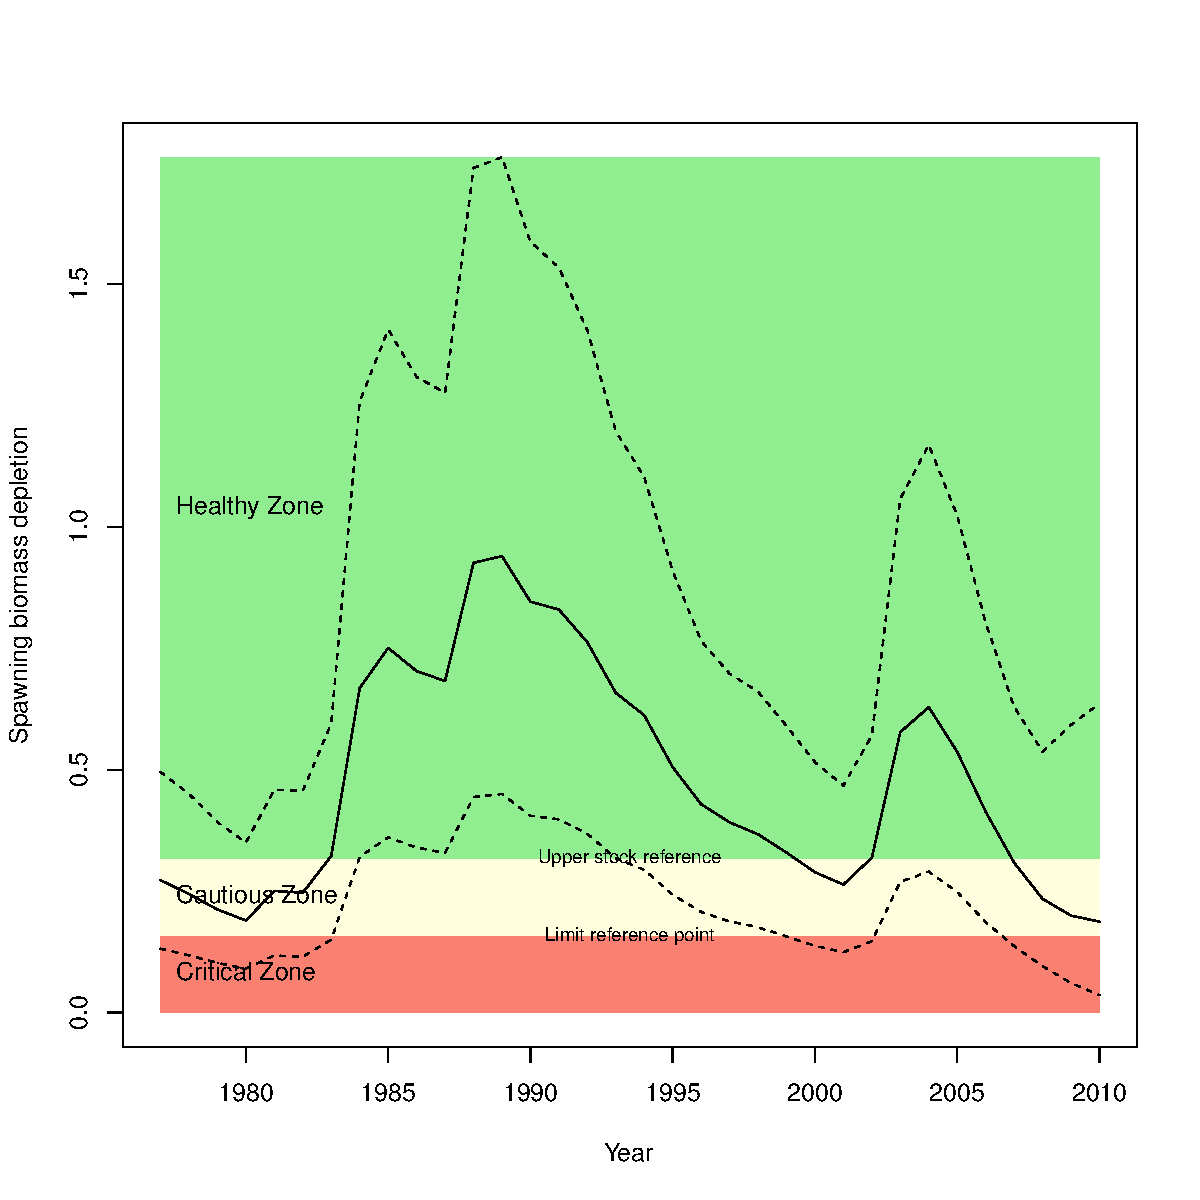
\includegraphics[width=\columnwidth]{iscamFigs/phakefig12.eps}\\
	\caption{Median estimates of spawning stock depletion and 95\% credible interval based 2000 samples from the joint posterior distribution. Transition between the critical, cautious and healthy zones is defined as 0.4\bmsy/$B_0$ and 0.8\bmsy/$B_0$, respectively }\label{fig16}
\end{figurehere}

\begin{scriptsize}
% latex.default(t1, "", file = filename, caption = cap, label = "iscam.T2") 
%
\begin{tablehere}
 \caption{Maximum likelihood estimates (MLE) and standard deviations (SD)
				based on the inverse Hessian for the six leading parameters. Median
				values and the 95\% credible interval based on posterior samples.\label{iscam.T2}} 
 \begin{center}
 \begin{tabular}{lrrrrr}\hline\hline
\multicolumn{1}{l}{}&\multicolumn{1}{c}{MLE}&\multicolumn{1}{c}{SD}&\multicolumn{1}{c}{Median}&\multicolumn{1}{c}{2.5\%}&\multicolumn{1}{c}{97.5\%}\tabularnewline
\hline
$\ln(R_0)$&$ 1.167$&$0.326$&$ 1.238$&$ 0.674$&$ 1.958$\tabularnewline
$h$&$ 0.688$&$0.214$&$ 0.669$&$ 0.370$&$ 0.932$\tabularnewline
$\ln(M)$&$-1.478$&$0.049$&$-1.457$&$-1.554$&$-1.363$\tabularnewline
$\ln(\bar{R})$&$-0.168$&$0.119$&$-0.103$&$-0.343$&$ 0.177$\tabularnewline
$\rho$&$ 0.293$&$0.043$&$ 0.305$&$ 0.227$&$ 0.405$\tabularnewline
$\vartheta$&$ 0.525$&$0.053$&$ 0.517$&$ 0.422$&$ 0.623$\tabularnewline
\hline
\end{tabular}

\end{center}

\end{tablehere}


\end{scriptsize}

\end{multicols}




Here is the data file for \iscam.
\tiny
\begin{alltt}
  \input{../PHake2010.dat}\label{HakeDataFile}
\end{alltt}
\normalsize


%    %!TEX root = /Users/stevenmartell/Documents/CURRENT PROJECTS/iSCAM-trunk/fba/BC-herring-2011/WRITEUP/BCHerring2011.tex
\section{Methods}
	\subsection{Input data \& assumptions}
	\subsubsection{Catch data}
	For each of the statistical areas, the required input data for \iscam\ consists of a catch time series for each of the fishing fleets.  For the BC herring fishery, the annual total removals has been partitioned into three distinct fishing fleets (or fishing periods, see Figure \ref{FigCatch}).  The first fleet is a winter seine fishery that has been in operation since the start of the assessment in 1951, the second is a seine-roe fishery that commenced in 1972 in the Strait of Georgia, and the third fleet is a gillnet fishery that targets females on the spawning grounds. The model is fit to the catch time series information and assumes measurement errors are lognormal, independent and identically distributed.  The assumed standard deviation in the catch observations must be specified in the control file and it is assumed that measurement errors in the catch is the same for all fishing periods.  The units of the catch are given in 1000s of metric tons.
	
	In addition to the commercial catch, removals from fisheries independent surveys must also be specified in \iscam. Two additional fleets are specified to represent the spawn survey, where the spawn survey is broken into two distinct time periods pre-1988 and post-1988, the year when the survey switched from surface surveys to dive surveys.  This partitioning of the data is done for two reasons: (1) to allow for different catchability coefficients to be specified for the early and late periods, and to allow for more weight to be placed on the contemporary data due to improved precision in the estimates of egg layers. 

%TODO decide if the test fishery data is going to be looked at here or in the appendix
	In the case where the test fishery data has been separated from the seine roe fishery, an additional fleet is specified in the data file and fishing mortality rates for the test fishery are also estimated in years when the catch is greater than 0.
	
\begin{figure}[!tbp]
	% Requires \usepackage{graphicx}
	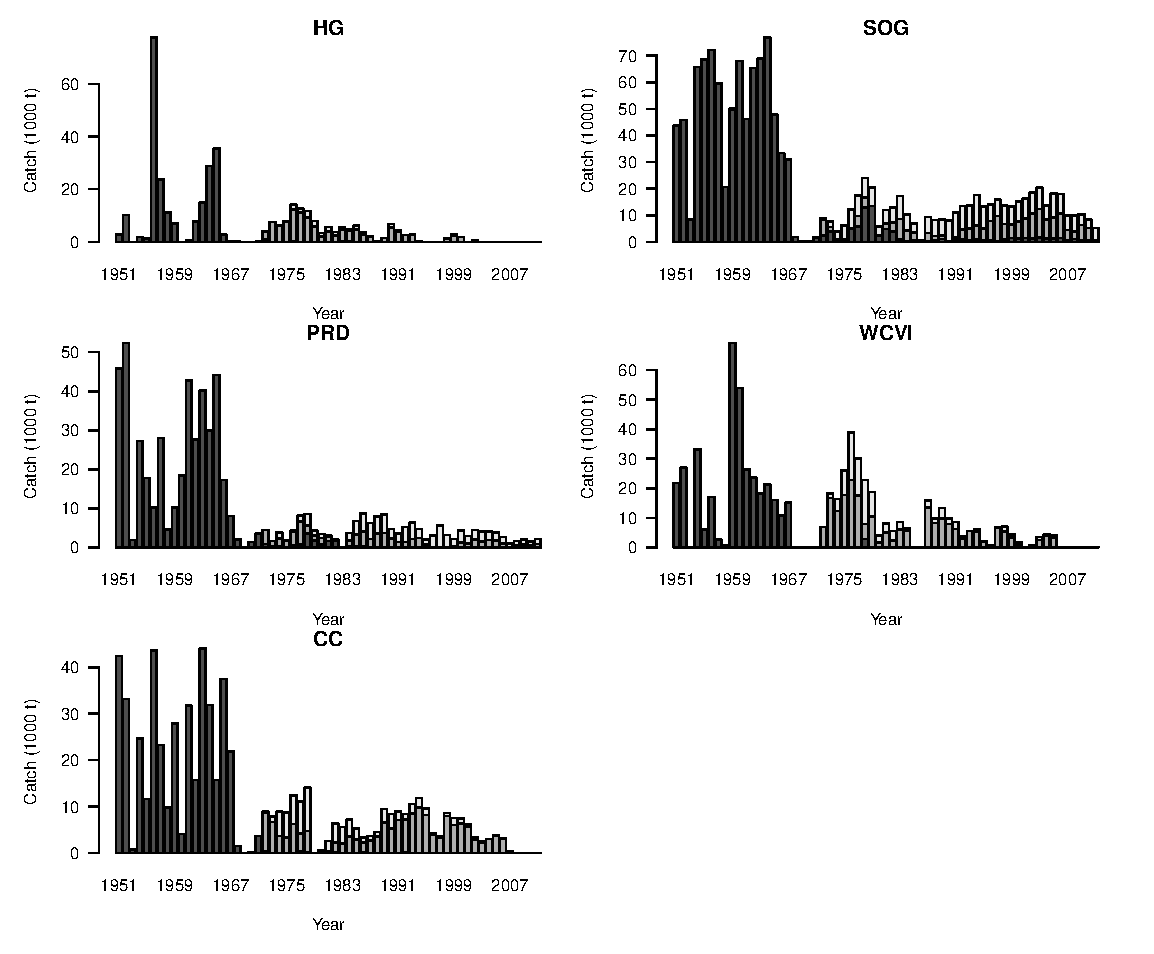
\includegraphics[width=\textwidth]{../Figs/iscam_fig_CatchMajorAreas.pdf}\\
	\caption{Historical catch of herring in the five major stock areas between 1951 and 2011 for the winter purse seine fishery (dark bars), seine-roe fishery (grey bars), and gillnet fishery (light grey bars). Units of catch are in thousands of metric tons.}\label{FigCatch}
\end{figure}
	
	\subsubsection{Relative abundance data}
Herring spawn surveys have been conducted throughout the B.C. coast beginning in the 1930s. Prior to 1988, spawn surveys were conducted from the surface either by walking the beach at low tide or using a drag from a skiff to estimate the shoreline length and width of spawn. Egg layers were sampled visually and are used to calculate egg densities following the methods of \cite{schweigert2001stock}. Beginning in 1988, herring spawn surveys using SCUBA methods were introduced and were implemented coastwide within a couple of years initially being conducted by DFO staff and eventually through contract divers hired through the test fishing program. Prior to the 2006 Larocque ruling, the test fishing program was funded through an allocation of fish by industry. In years since the 2006 Larocque ruling, the availability of resources to conduct dive surveys in all areas has been reduced. For 2011, dive surveys were conducted in all major and minor assessment regions, with the exception of Area 2W where snorkelling and surface survey methods were also used. As in earlier years, a few minor spawning beds outside the main assessment areas were surveyed by SCUBA or surface methods where resources permitted.


The locations of the spawning beds for the five major and two minor stock areas are shown in Figure \ref{figSpawnMaps}.  Egg density estimates are used to calculate a fishery-independent index of herring spawning biomass, referred to as the spawn survey index hereafter \citep{schweigert2001stock}.

\begin{figure}[!tbp]
	% Requires \usepackage{graphicx}
	\centering
	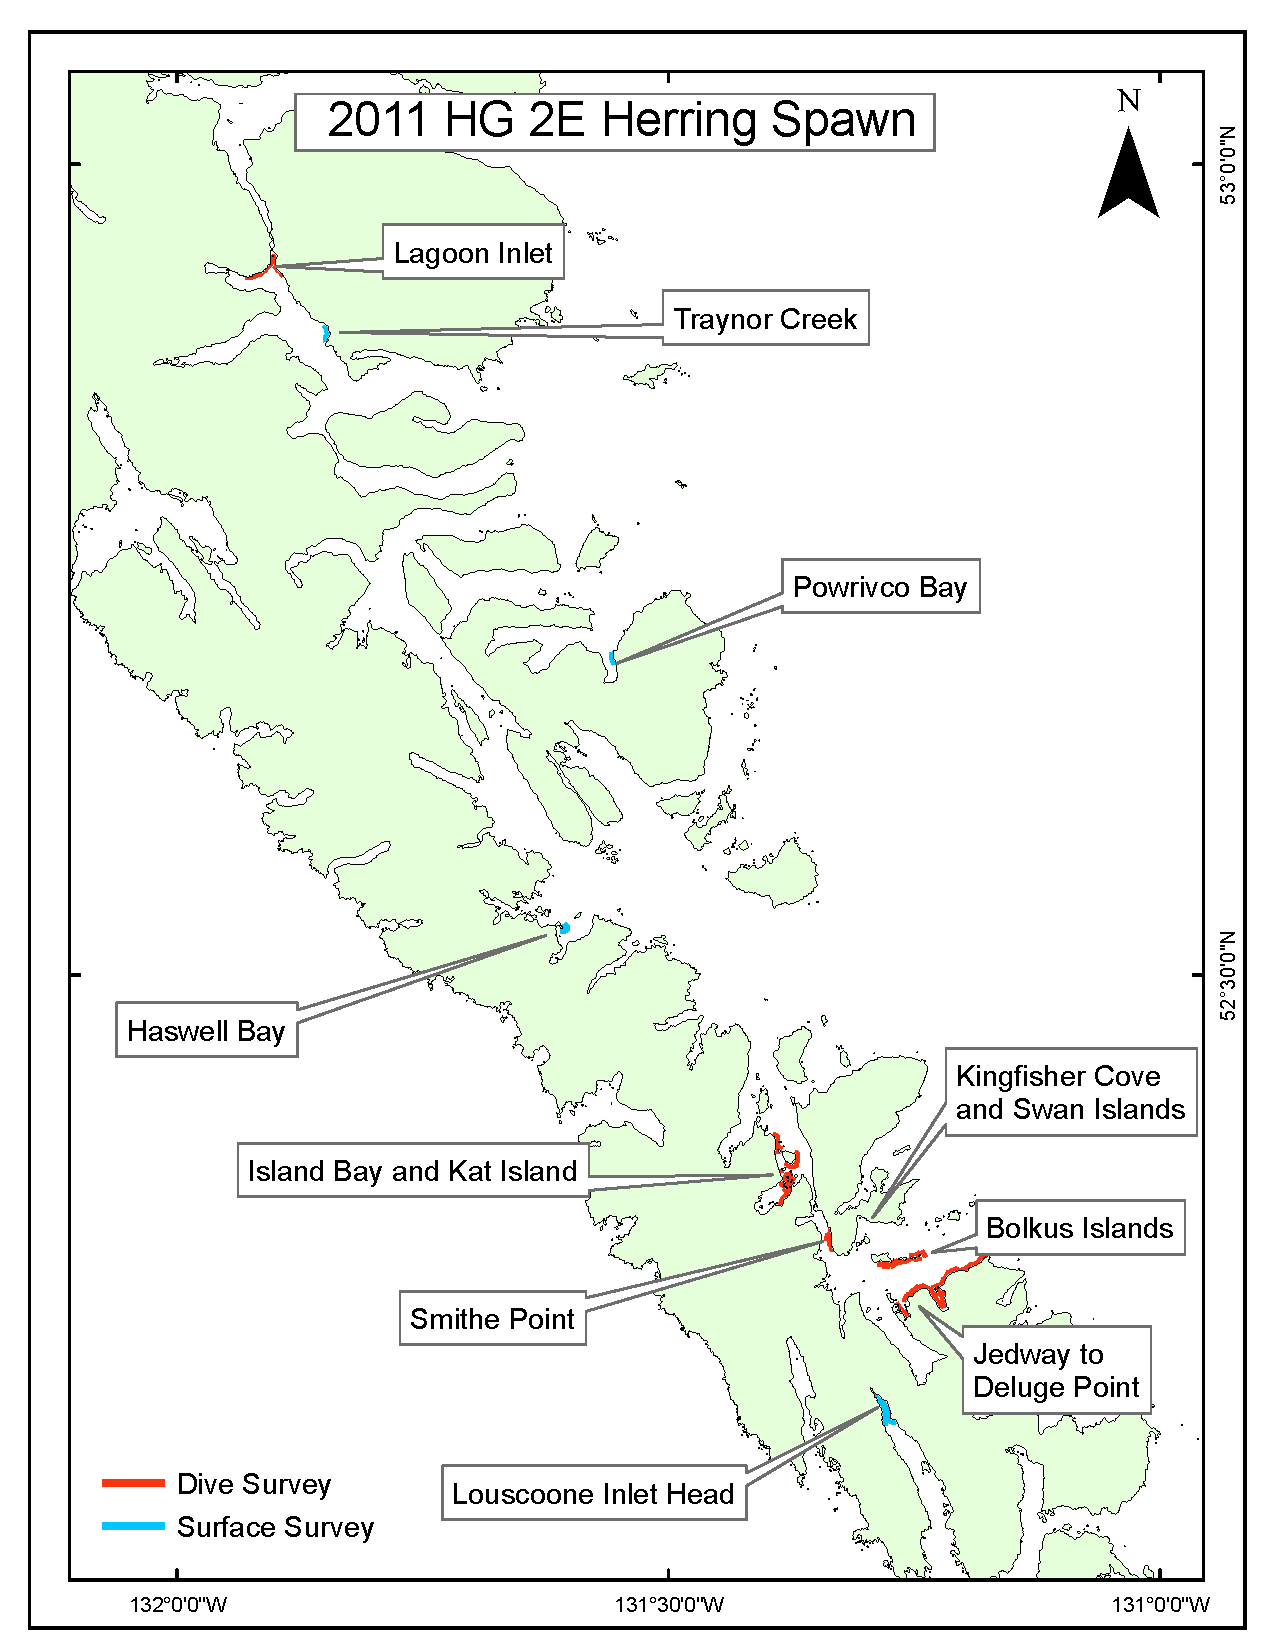
\includegraphics[scale=0.35]{../Figs/PBSfigs/2011_spawn_HG_2E_July13.pdf}
	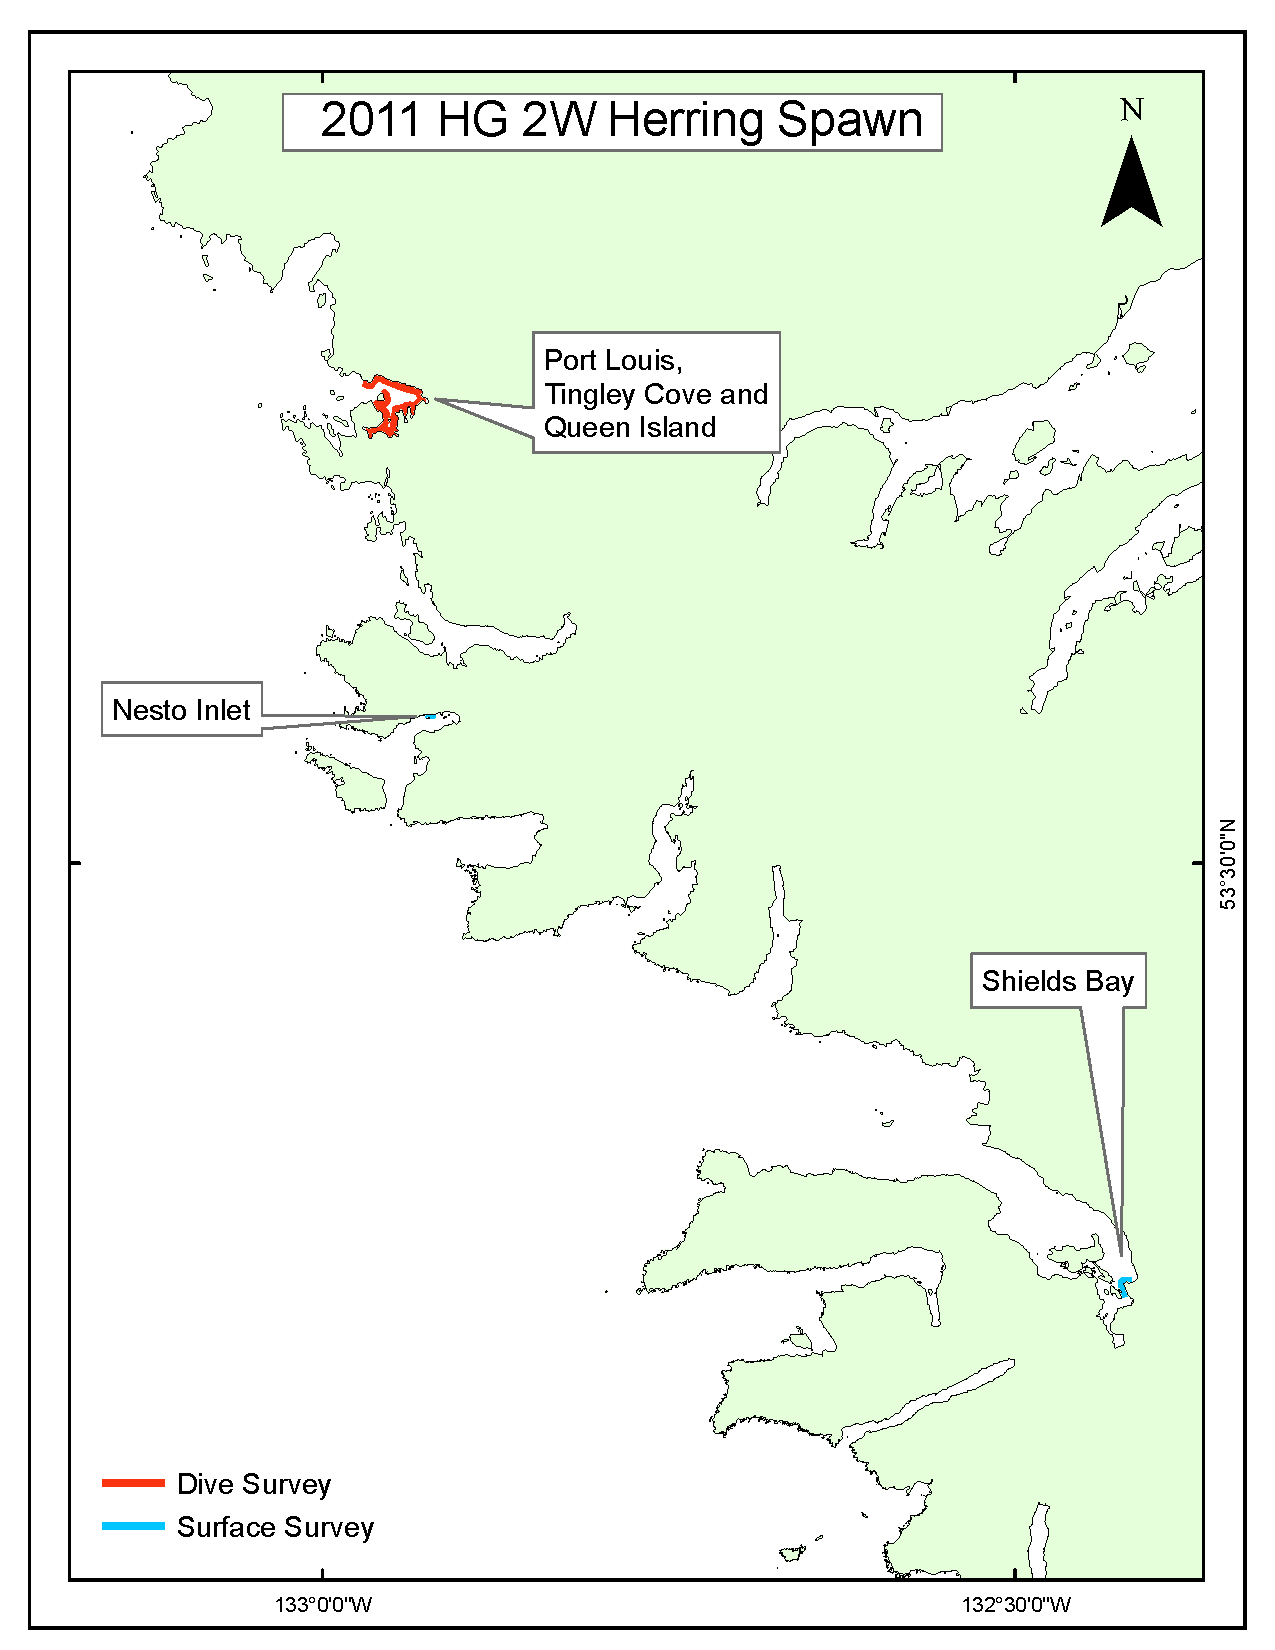
\includegraphics[scale=0.35]{../Figs/PBSfigs/2011_spawn_HG_2W_July13.pdf}\\
	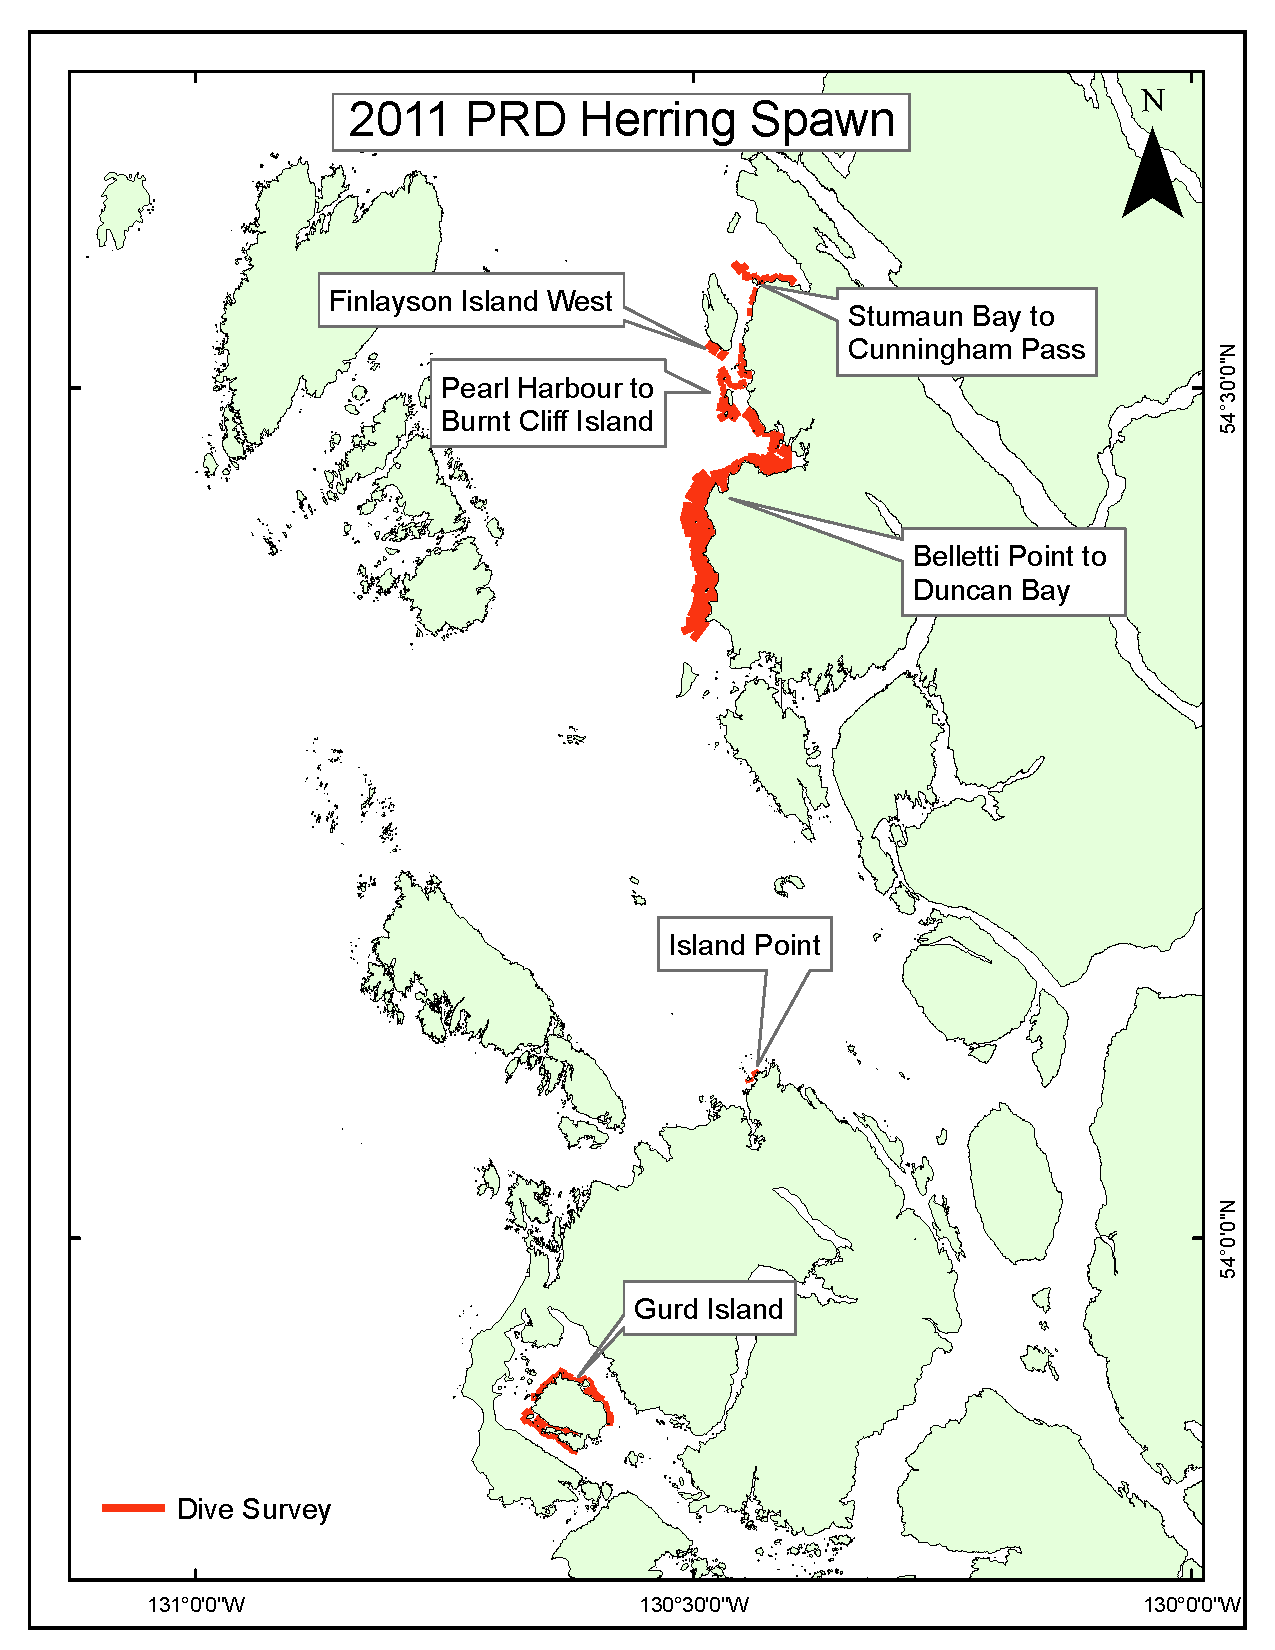
\includegraphics[scale=0.35]{../Figs/PBSfigs/2011_spawn_PRD_July13.pdf}
	\caption{Preliminary Spawning activity for Haida Gwaii (top panels) and Prince Rupert District (bottom) in 2011.}
\end{figure}
\begin{figure}[!tbp]
	% Requires \usepackage{graphicx}
	\ContinuedFloat
	\centering
	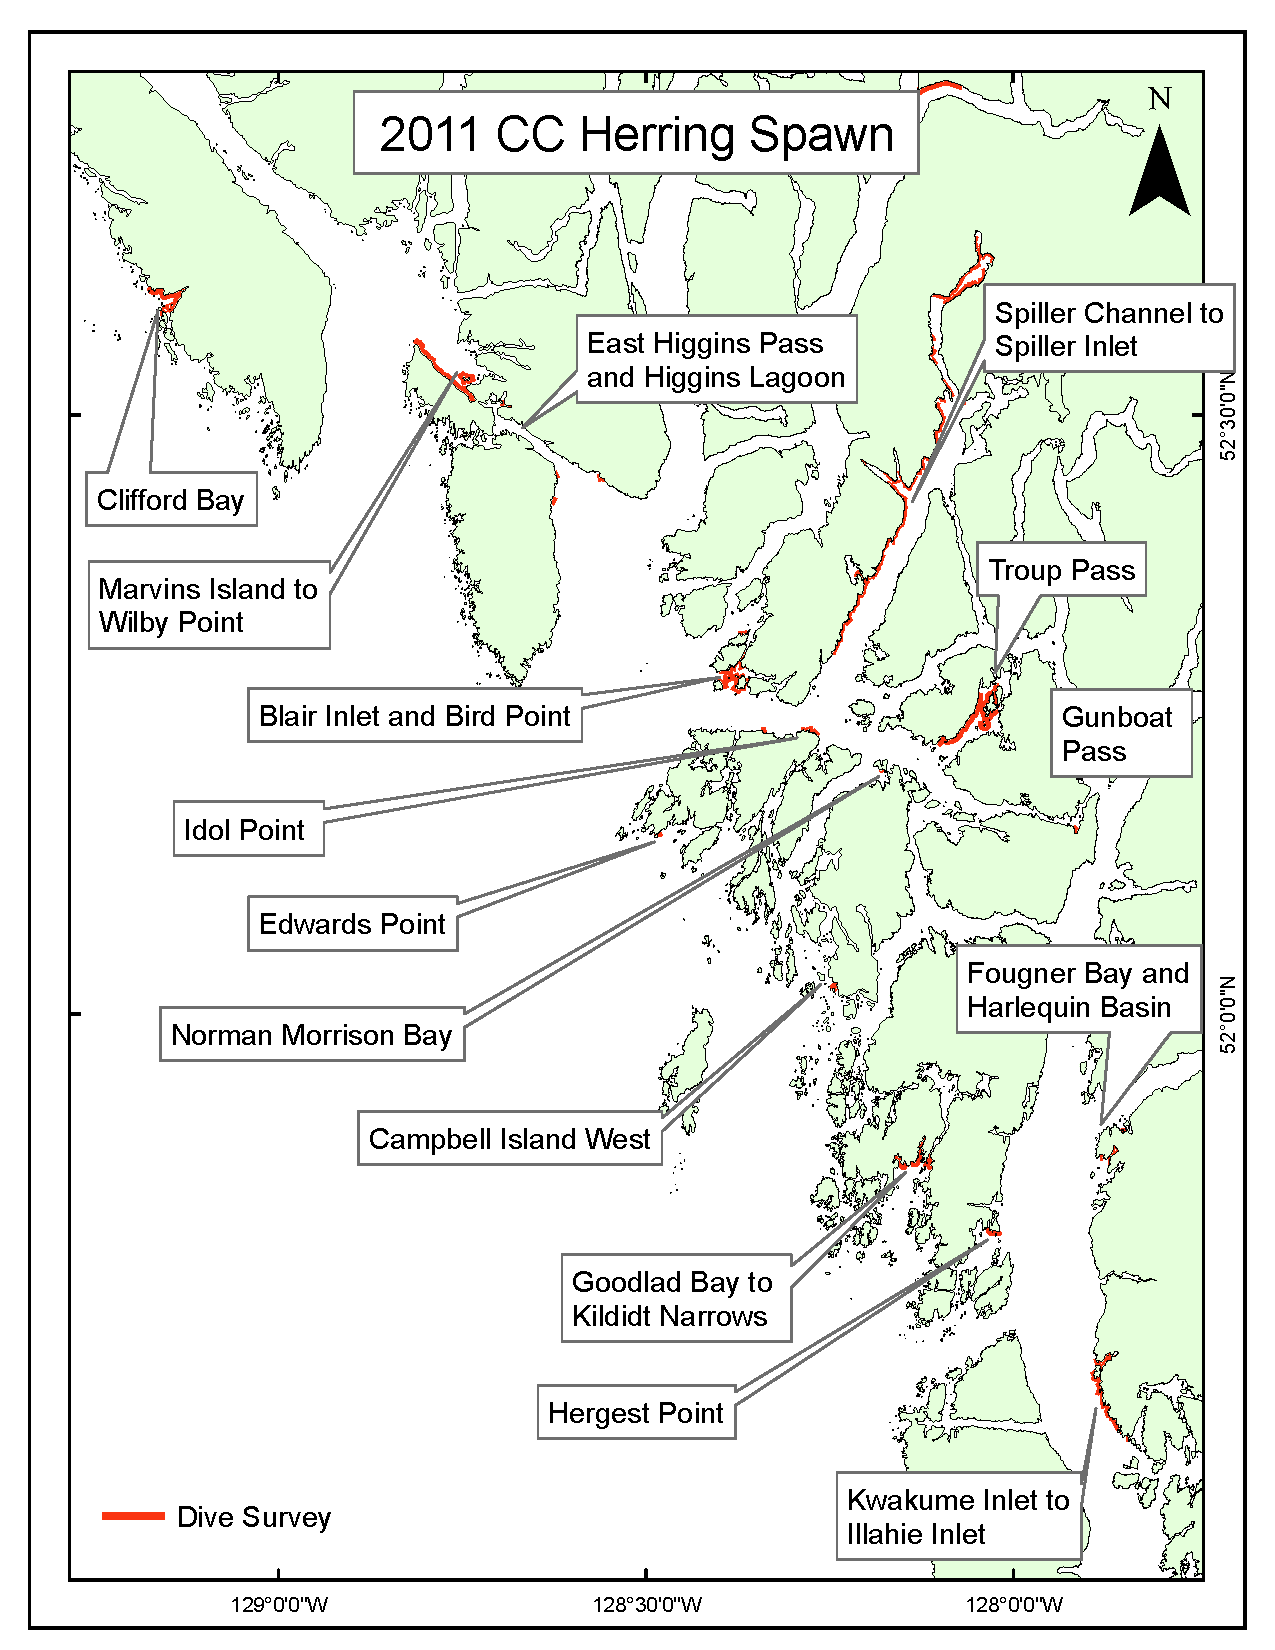
\includegraphics[scale=0.35]{../Figs/PBSfigs/2011_spawn_CCJuly13.pdf}
	%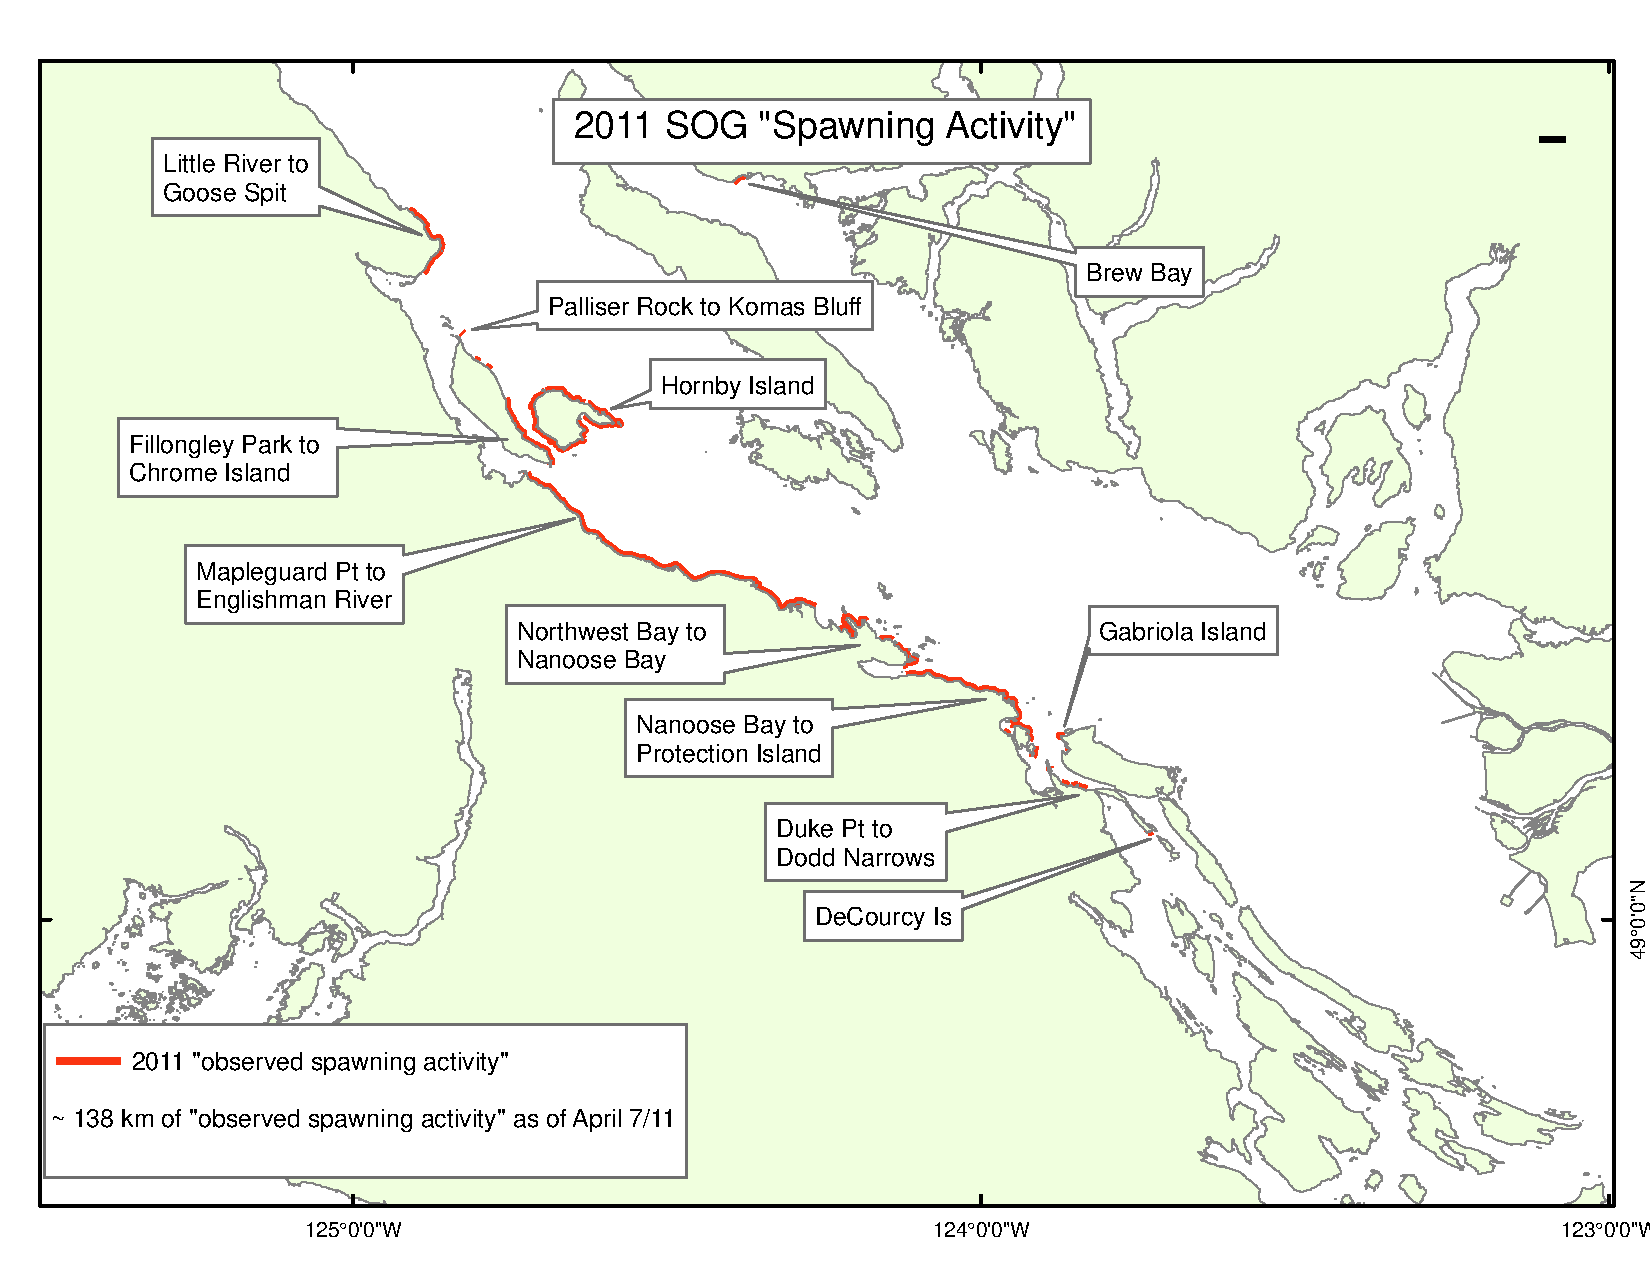
\includegraphics[scale=0.5]{../Figs/PBSfigs/2011-SOG-Prelim-WG.pdf}
	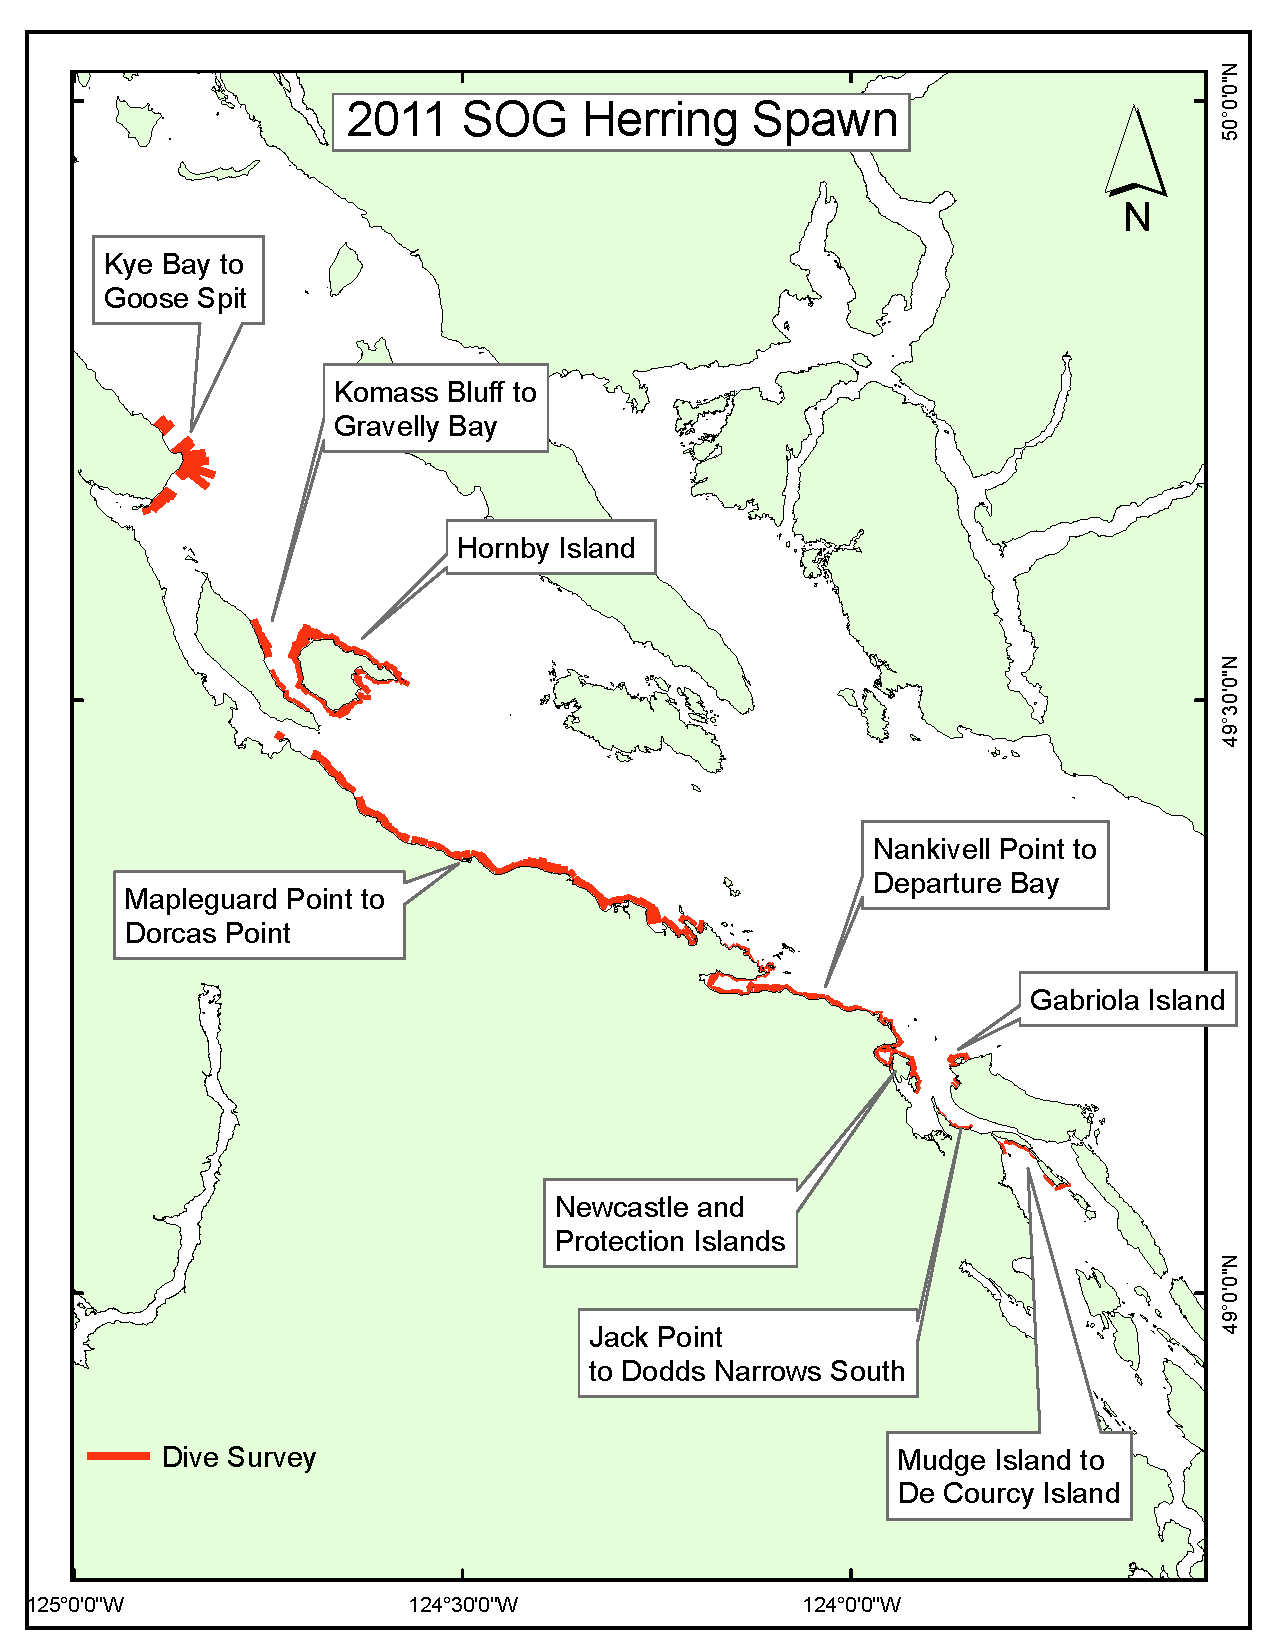
\includegraphics[scale=0.35]{../Figs/PBSfigs/2011_spawn_SOG_July13.pdf}\\
	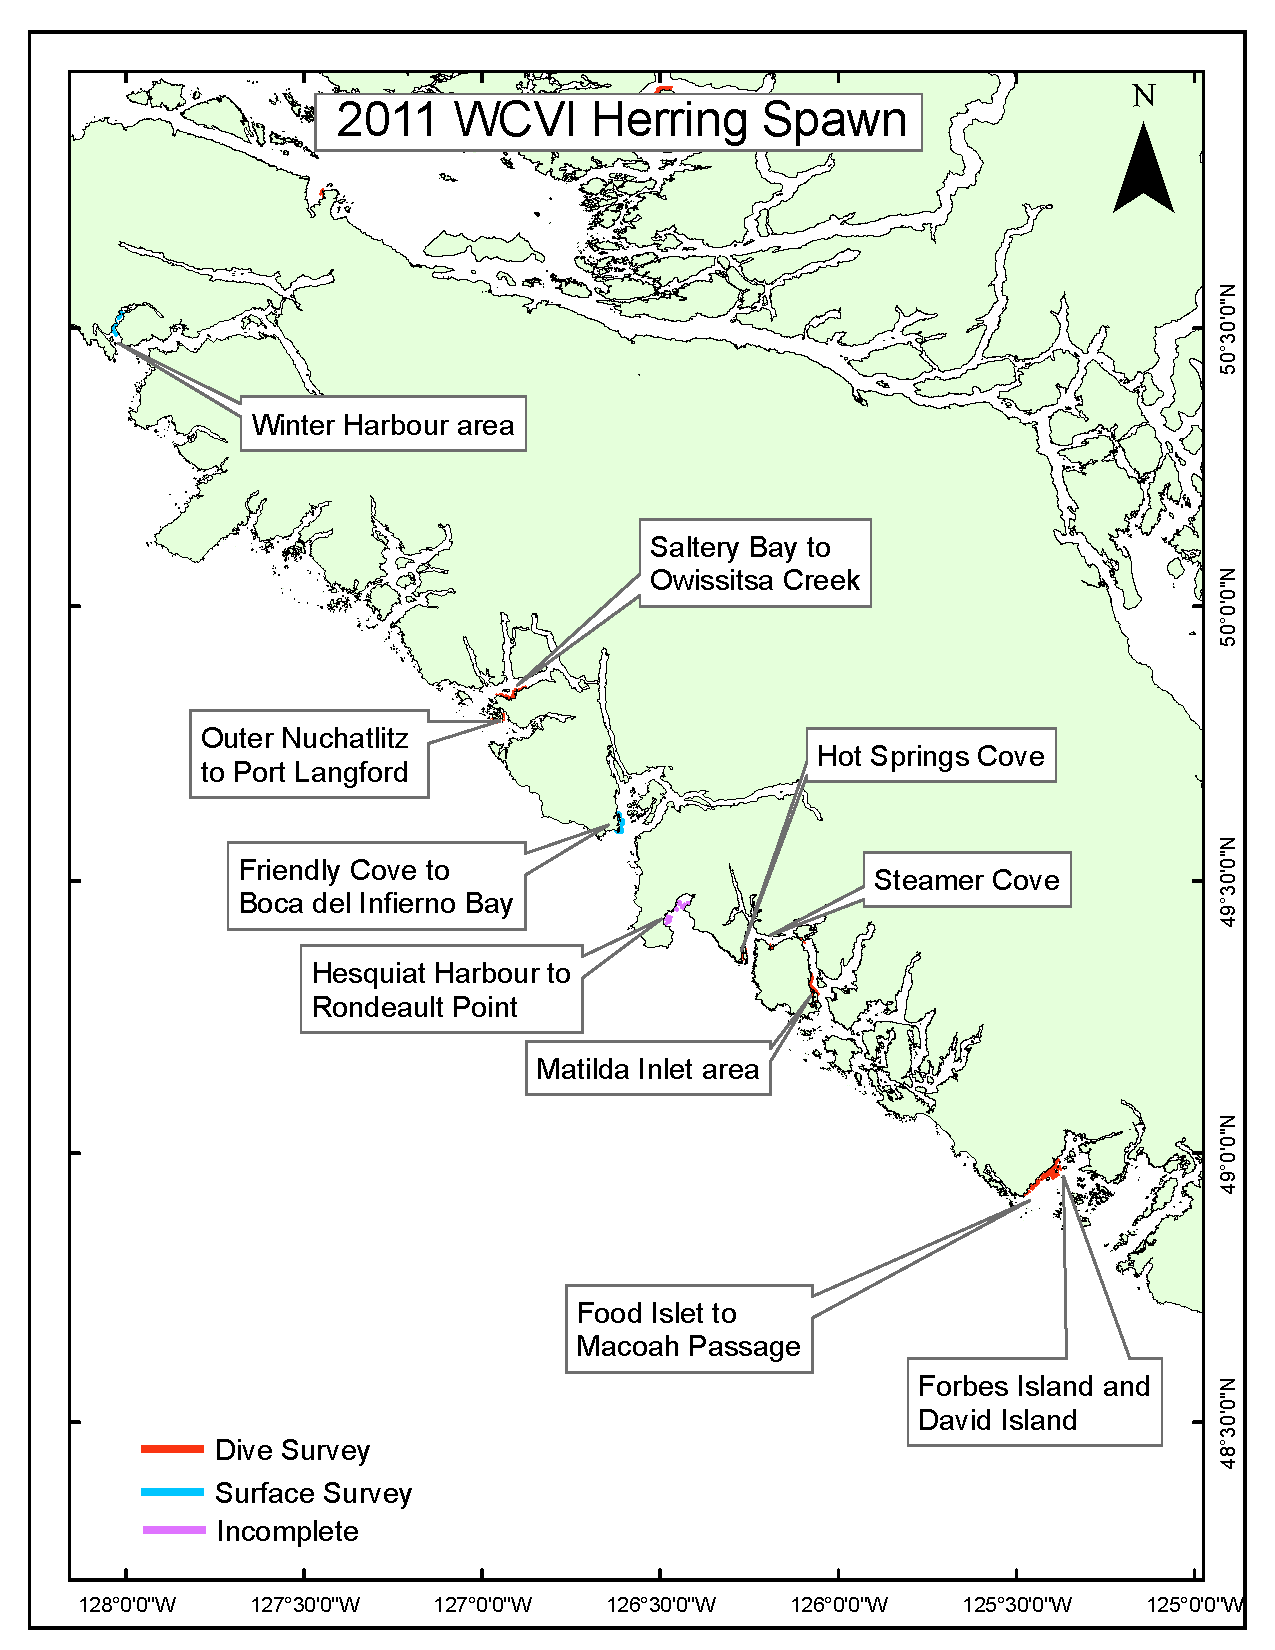
\includegraphics[scale=0.35]{../Figs/PBSfigs/2011_spawn_WCVI_August16.pdf}
	\caption{Preliminary Spawning activity for Central Coast (top left panel), Strait of Georgia (top right) in 2011 and west coast Vancouver Island (bottom).}\label{figSpawnMaps}
\end{figure}
% \begin{figure}[!tbp]
% 	% Requires \usepackage{graphicx}
% 	\ContinuedFloat
% 	\centering
% 	%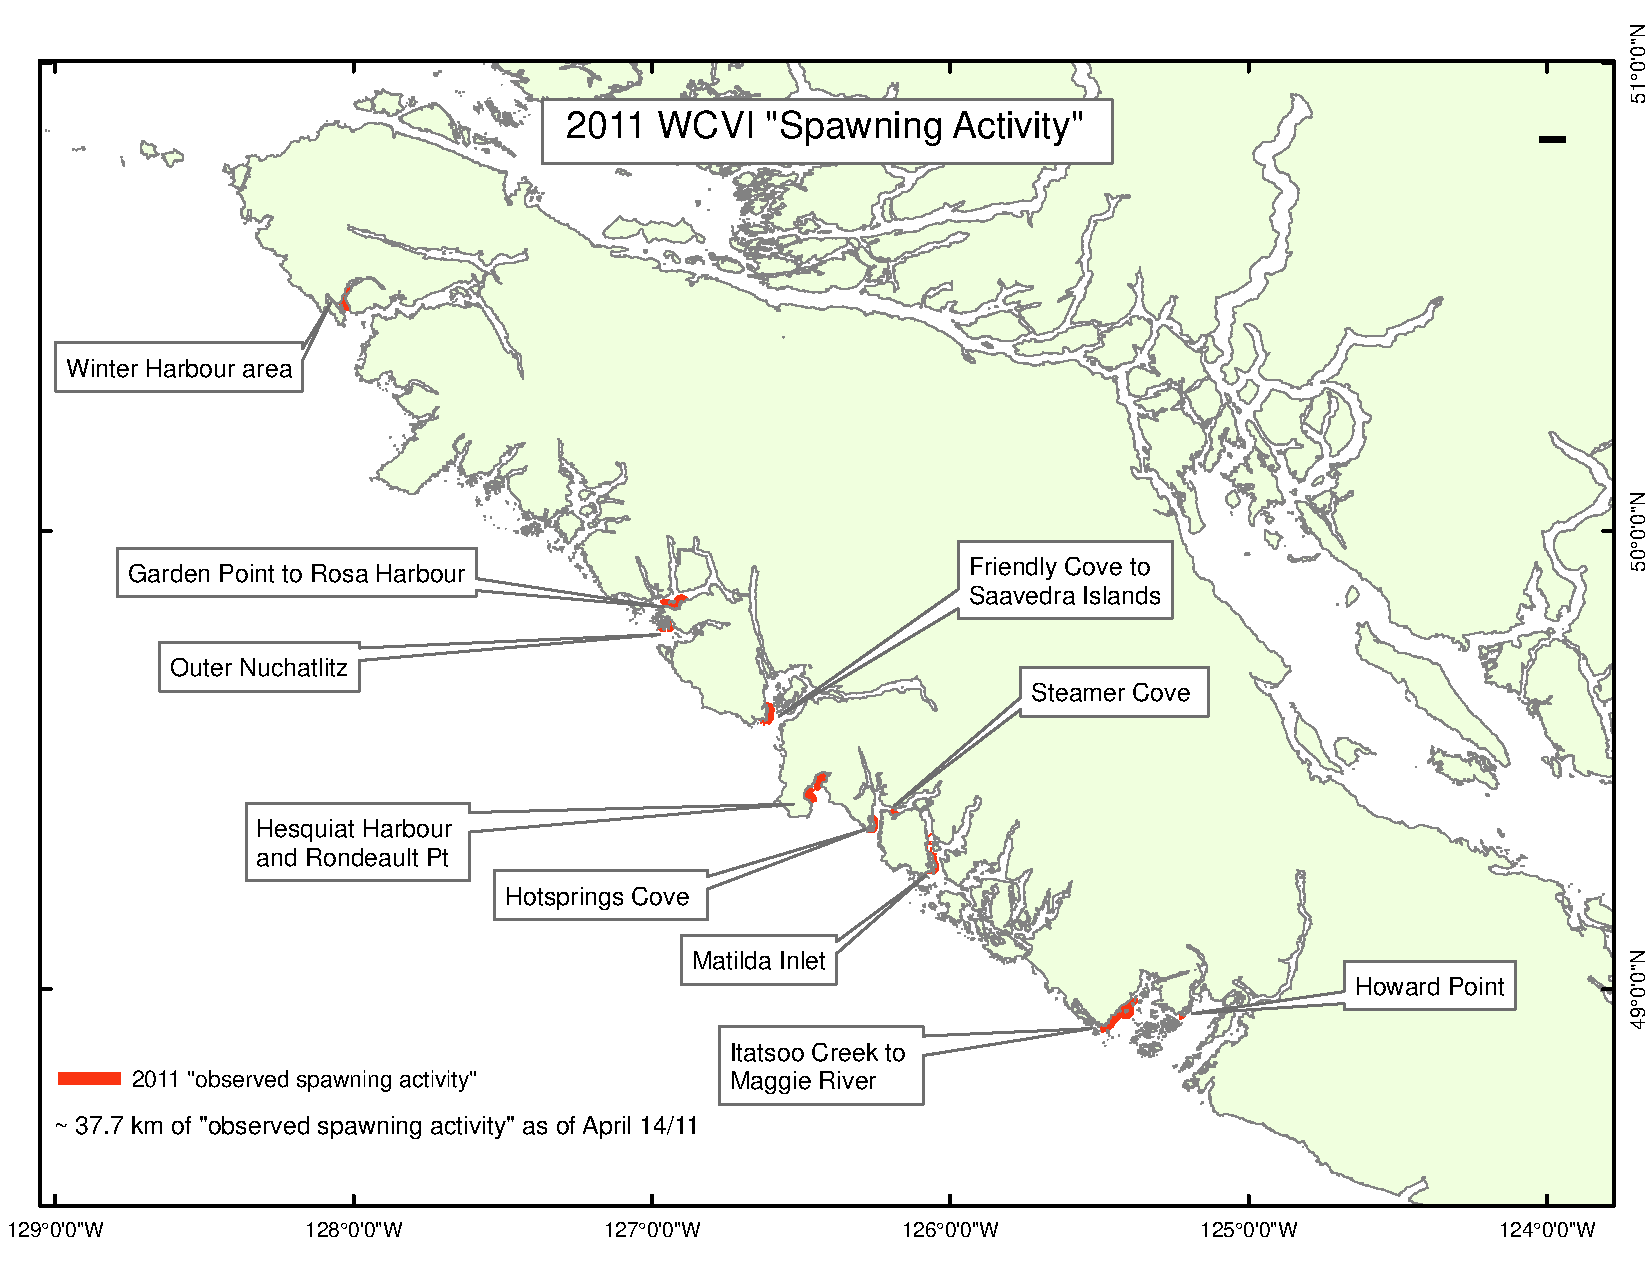
\includegraphics[scale=0.5]{../Figs/PBSfigs/2011-WCVI-Prelim-WG.pdf}\\
% 	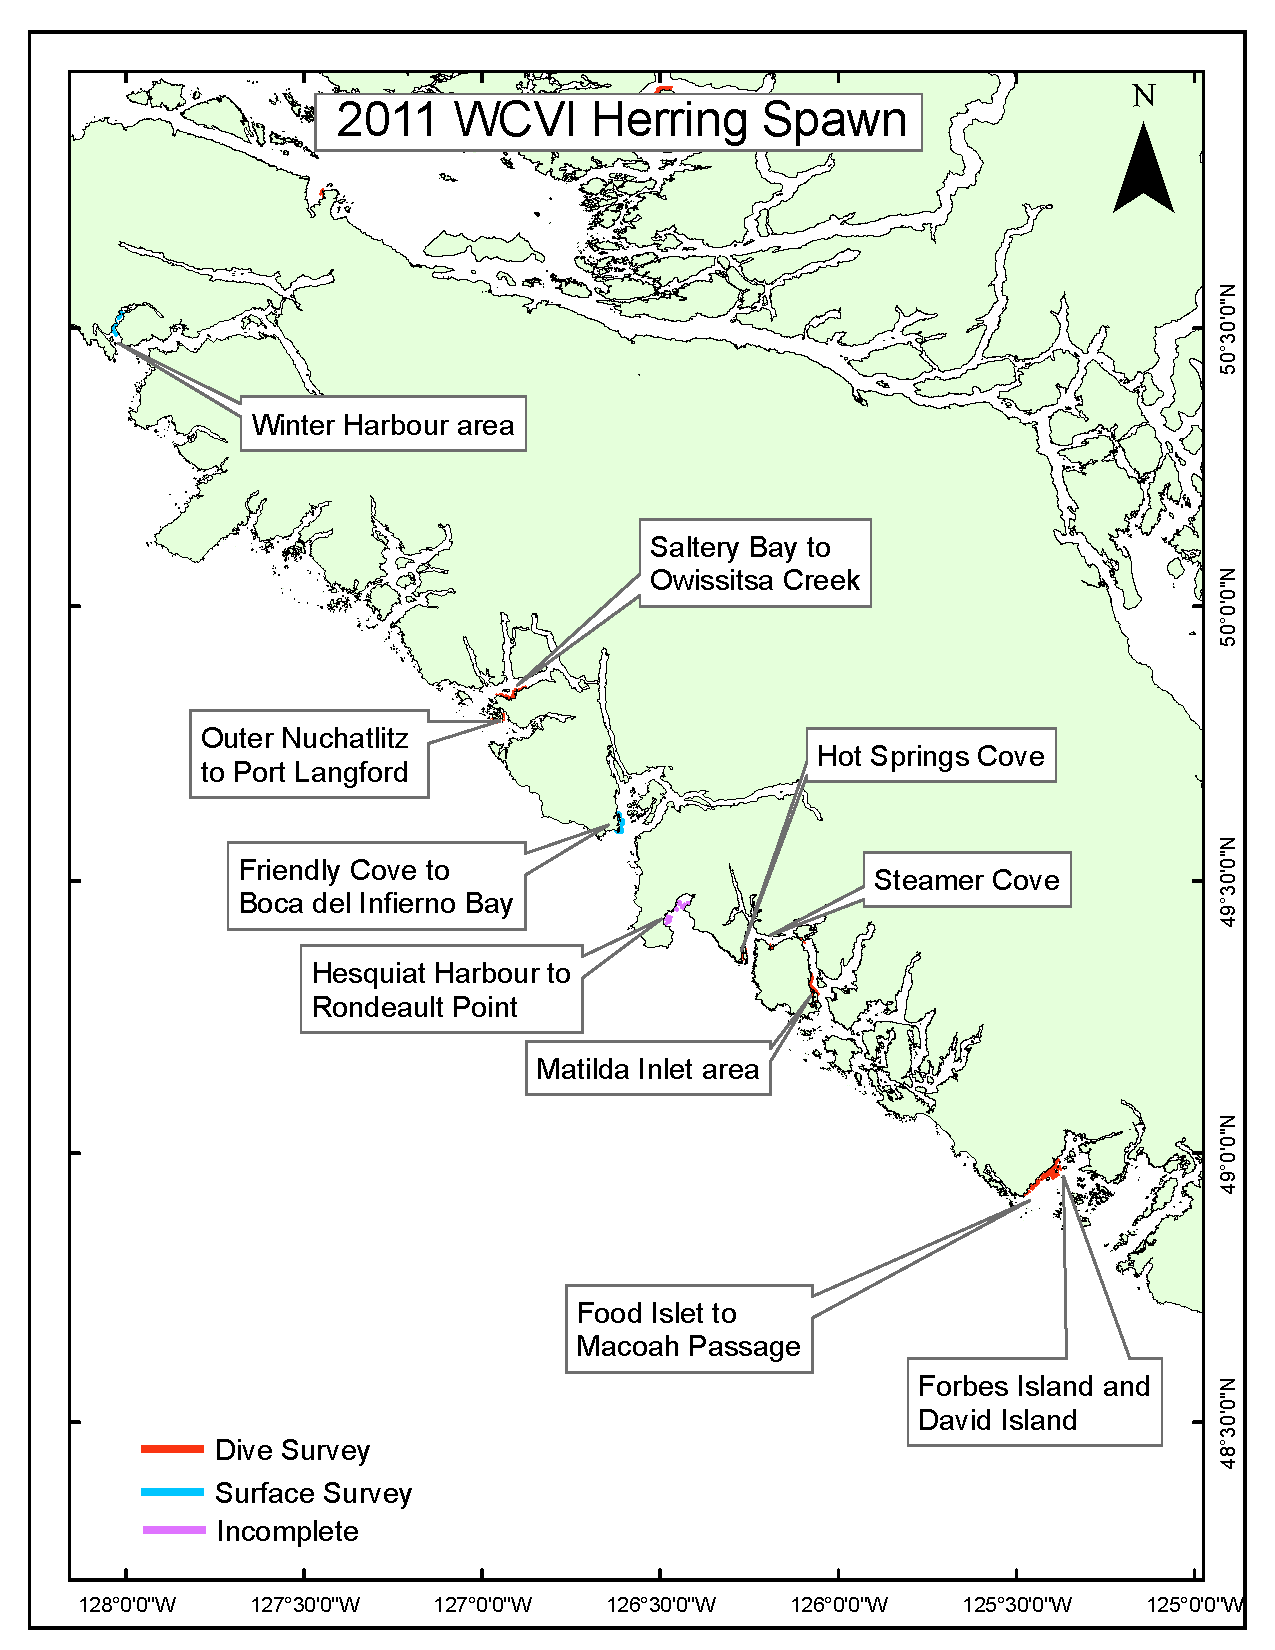
\includegraphics[scale=0.5]{../Figs/PBSfigs/2011_spawn_WCVI_August16.pdf}\\
% 	\caption{Preliminary Spawning activity in 2011 for the West Coast of Vancouver Island (includes minor stock area 27).}\label{figSpawnMaps}
% \end{figure}

	The spawn survey is conducted after the fisheries in the area have been completed; therefore, it is assumed that all the mortality for the year has occurred just prior to commencing the spawning survey. The fisheries independent survey estimates egg density and total spawn area, and from this information the total female spawning biomass can be estimated assuming the 200 eggs per gram of female  or 100 eggs per gram of mature  individuals \citep{hay1985reproductive,hardwick1973biomass}. The assumed selectivity for the spawn survey is fixed to the maturity schedule for herring.  	
	
\begin{figure}[!tbp]
	% Requires \usepackage{graphicx}
	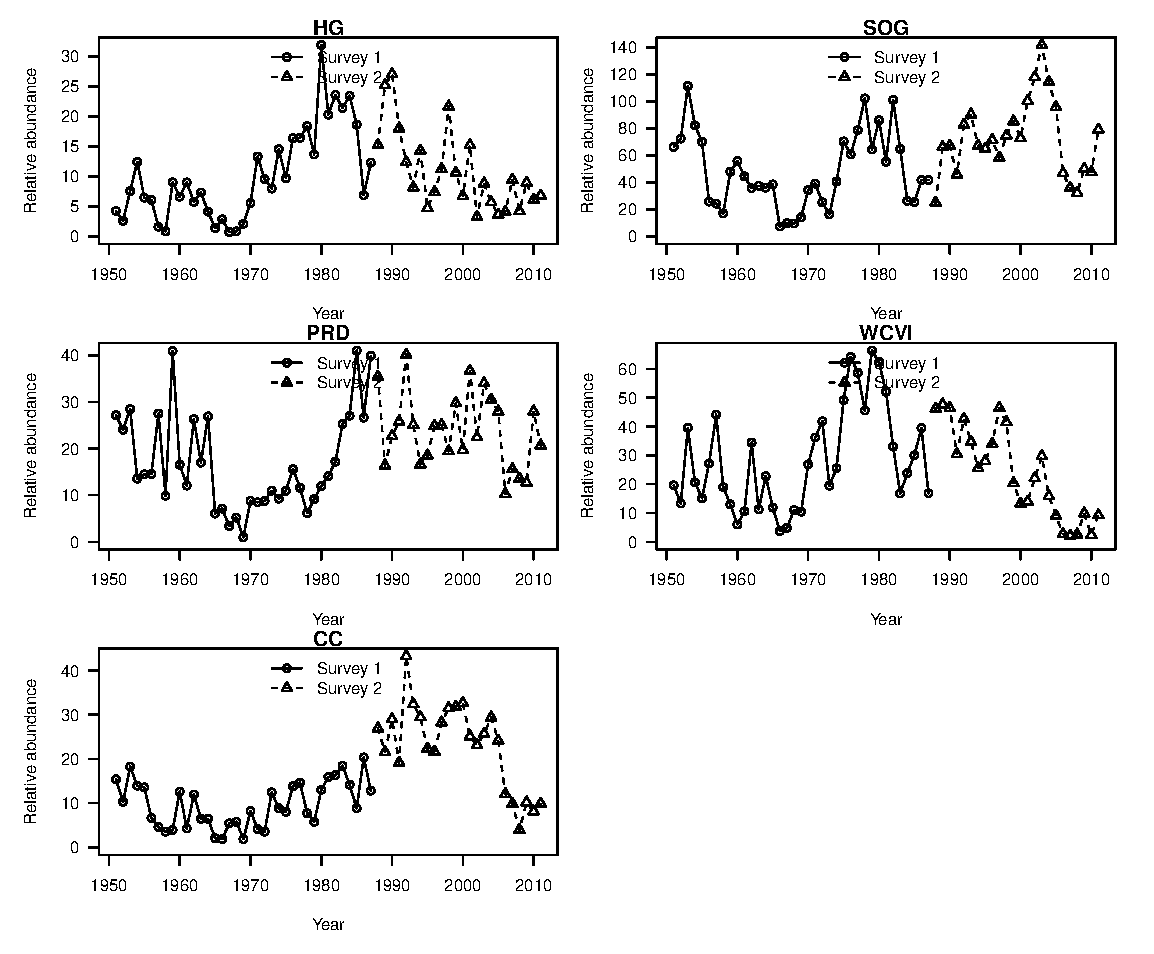
\includegraphics[width=\textwidth]{../Figs/iscam_fig_SurveyMajorAreas.pdf}\\
	\caption{Spawn survey index for Strait of Georgia between 1951 and 2011. The units are actual estimates of spawning biomass (1000s tons), but only the trend information is used in the model fitting.}\label{FigSurvey}
\end{figure}
	
	\subsubsection{Biological samples}
	
	Biological samples are collected from both commercial catch and from the test fishery program.  Commencing  in 1975, test fishery charters supplemented biological samples in areas with poor sampling that was not representative of the stock in that area (i.e., fishing solely on spawning aggregations), or in closed areas. Prior to 2006, test fishing charters were funded through an allocation of fish to the test program; the program is now fully funded by DFO.  Through a contract with DFO, the Herring Conservation and Research Society (HCRS) sub-contracts a number of vessels to collect biological samples.  Industry also conducts pre-season test sets for roe-quality testing in open areas and supplementary biological samples are provided as part of this program.  The following data are collected for all biological samples: fish length, weight, sex, and maturity.  Subsequently these sources of data are combined and information on weight-at-age and proportion-at-age become input data for the stock assessment model.
	
	During the 2010/2011 season a total of 248 biological samples were collected, of which 151 were collected from the test fishery, 57 were collected from the roe fishery, 16 from the food \& bait fishery, 4 from Spawn on Kelp (SOK) operations, and 16 from the summer trawl research survey (Table \ref{table:PartII:bioSamples}).  Note that the definition of a sample is roughly 100 individual fish.  A summary of biological samples collected from commercial and pre-fishery charters from 2002/03--2010/11 is presented in Table \ref{table:PartII:sampleSizes}).

\begin{table}
	\caption{Summary of biological samples collected and processed from all sources from the 2010/11 herring season.}
	\label{table:PartII:bioSamples}
	\begin{center}
		\begin{tabular}{cccccc}
		\hline
		& \multicolumn{3}{c}{Commercial samples} &  \\
		Stock & Roe fishery & SOK fishery & F\&B & Test fishery & Research\\
		\hline
		HG (QCI 2E) &  &  &  & 13\\
		PRD & 29 & 1 &  & 24\\
		CC &  &  &  & 30\\
		SOG & 18 &  & 20 & 60\\
		WCVI &  &  &  & 14 & 16\\
		Area 2W &  &  &  & 10\\
		Area 27 &  & 3\\
		Other Areas\\
		\hline
		Total & 57 & 4 & 16 & 151 & 16\\
		\hline
		\end{tabular}
	\end{center}
\end{table}

\begin{table}
	\caption{Summary of biological samples collected and processed from commercial catch and test fishery charters from 2002/03-2010/11.}
	\label{table:PartII:sampleSizes}
	\begin{center}
\begin{tabular}{cccc}
\hline
Fishing season & Commercial fishery samples & Charter and research samples & Total\\
\hline
2002/03 & 120 & 287 & 407\\
2003/04 & 79 & 222 & 301\\
2004/052 & 83 & 191 & 274\\
2005/06 & 46 & 164 & 210\\
2006/07 & 114 & 85 & 199\\
2007/08 & 116 & 103 & 219\\
2008/09 & 87 & 136 & 223\\
2009/10 & 78 & 135 & 213\\
2010/11 & 81 & 167 & 248\\
\hline
\end{tabular}
	
	\end{center}
\end{table}
	
	
	
	%%Insert Summary of biological samples from the 2010/2011 season here:
	
	%%Insert Summary of biological samples collected and processeed from commercial catch etc. here (Table 2 from Cleary 2011).
	
	\subsubsection{Age composition data}
	
	Ageing data, through the reading of fish scales, are collected from the biological samples taken from the commercial fisheries and test fishery charters. Age composition data is used to determine proportions-at-age and is an essential source of input data to the herring stock assessment model.
	
	Catch-at-age data from the winter seine fishery (top panels of Figures \ref{FigAgeCompsHG}-\ref{FigAgeCompsWCVI}) tend to consist of younger fish in comparison to the age composition data from the seine-roe and gillnet fleets post 1970. The shaded polygons in Figures \ref{FigAgeCompsHG}-\ref{FigAgeCompsWCVI} approximates the 95\% distribution of ages in the catch.  Roughly 90\% of the fish landed in the winter seine fishery were younger than age-7, and younger than age-6 in recent years.  In both the winter seine and seine-roe fishery age-2 fish are frequently landed; whereas, age-2 fish are rarely landed in the gillnet fishery, and fish do not appear to fully recruit to the gear until at least 4-5 years of age.  The mean age of the catch appears to be increasing between 2008 and 2010 in both the gillnet and winter seine fishery, and there is no obvious trend in the seine roe fishery.  There is however a declining trend in the older ages caught in the seine-roe fishery since 2006 (erosion of age-structure).

\begin{sidewaysfigure}[!tbp]
	% Requires \usepackage{graphicx}
	\centering
	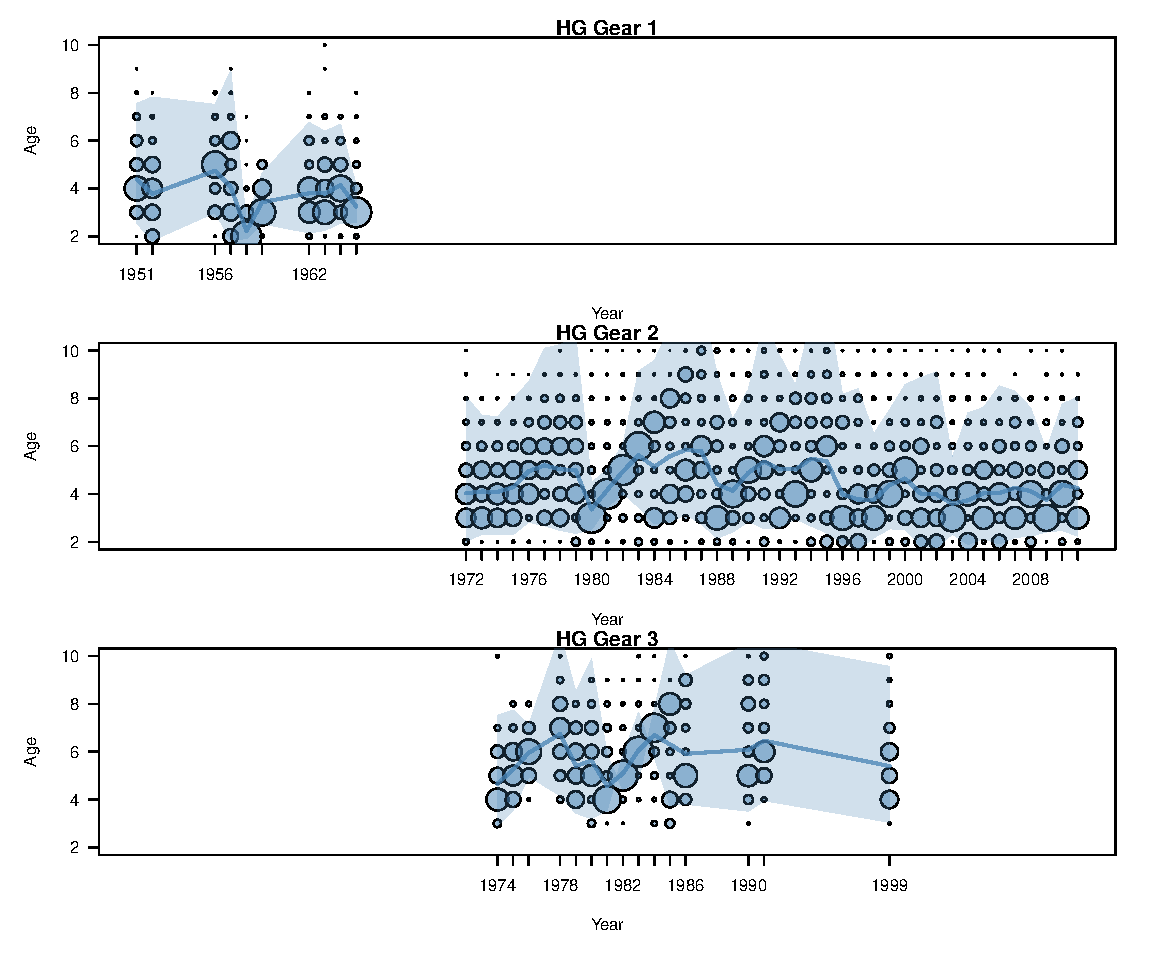
\includegraphics[width=0.85\textwidth]{../Figs/iscam_fig_AgeCompsHG.pdf}\\
	\caption{Bubble plots showing the proportions-at-age versus time for the winter purse seine fishery (top), seine roe fishery (middle) and the gillnet fishery (bottom) in Haida Gwaii.  The area of the circle is proportional to cohort abundance, each column sums to 1, zeros are not shown, and age 10 is a plus group. Also shown is the mean age of the catch (line) and the approximate 95\% distribution of ages (shaded polygon) for each year.}\label{FigAgeCompsHG}
\end{sidewaysfigure}

\begin{sidewaysfigure}[!tbp]
	% Requires \usepackage{graphicx}
	\centering
	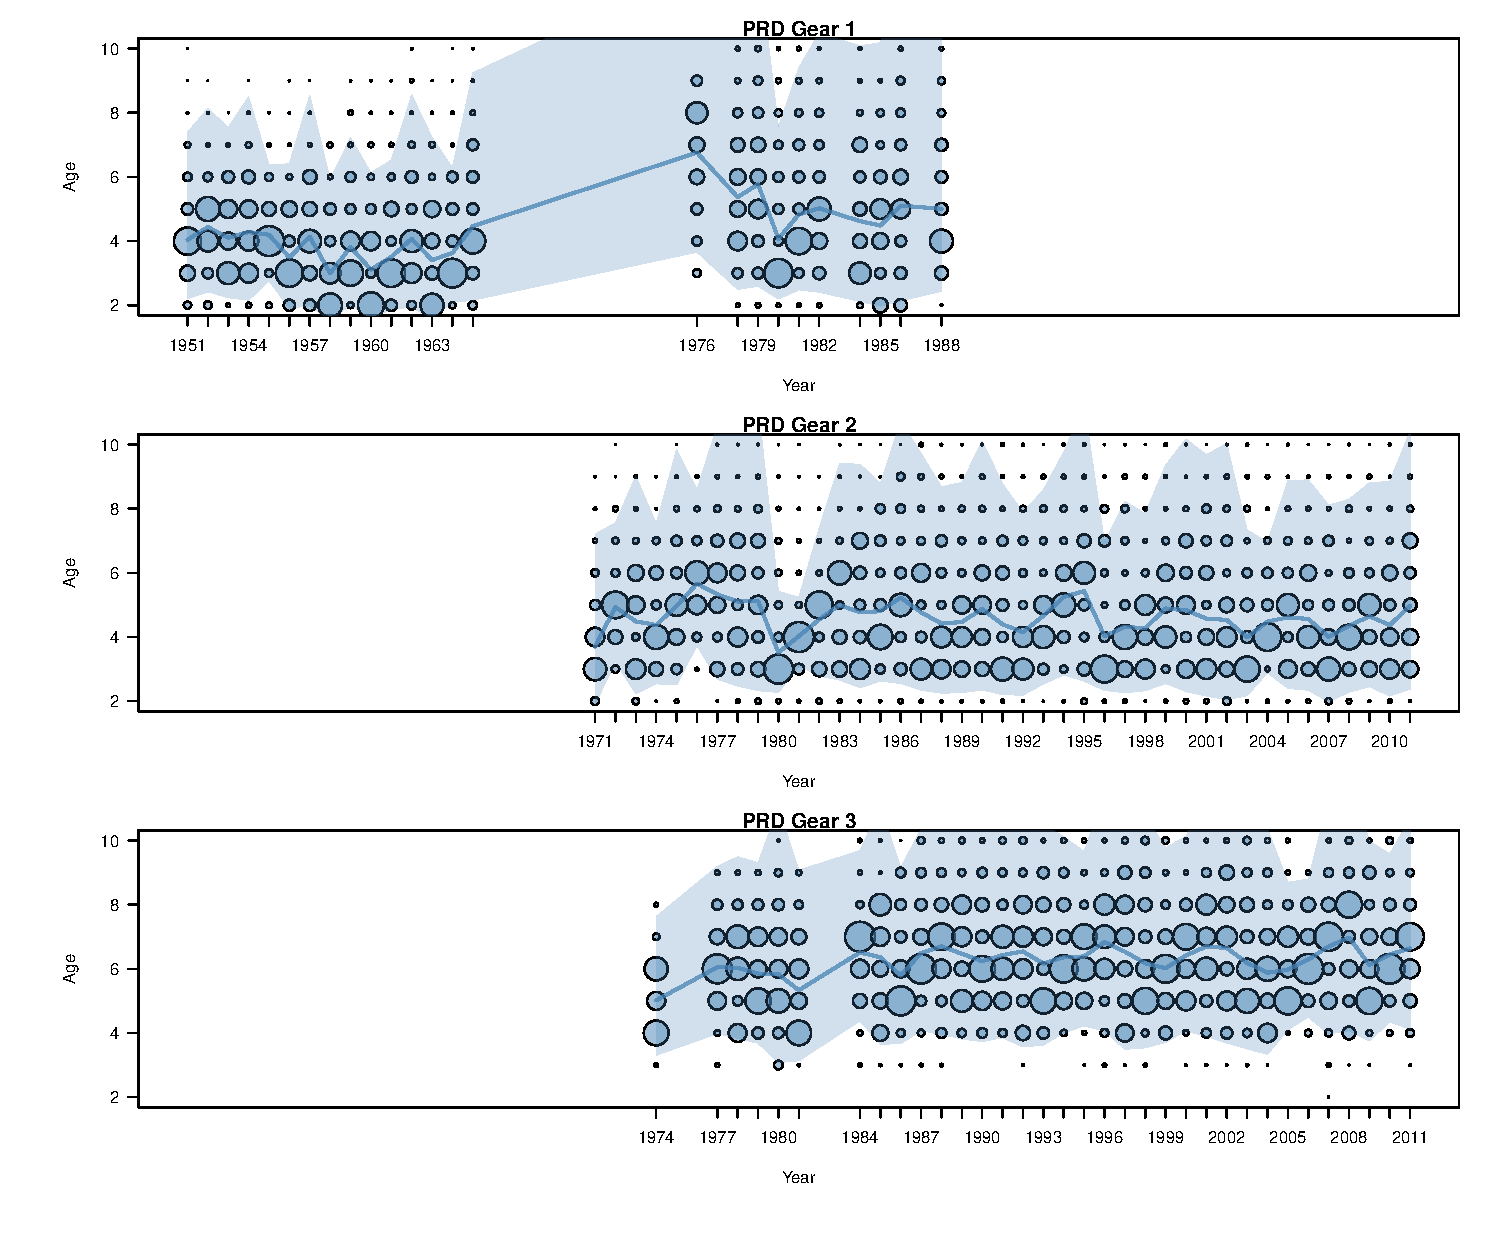
\includegraphics[width=0.85\textwidth]{../Figs/iscam_fig_AgeCompsPRD.pdf}\\
	\caption{Bubble plots showing the proportions-at-age versus time for the winter purse seine fishery (top), seine roe fishery (middle) and the gillnet fishery (bottom) in Prince Rupert District.  The area of the circle is proportional to cohort abundance, each column sums to 1, zeros are not shown, and age 10 is a plus group. Also shown is the mean age of the catch (line) and the approximate 95\% distribution of ages (shaded polygon) for each year.}\label{FigAgeCompsPRD}
\end{sidewaysfigure}

\begin{sidewaysfigure}[!tbp]
	% Requires \usepackage{graphicx}
	\centering
	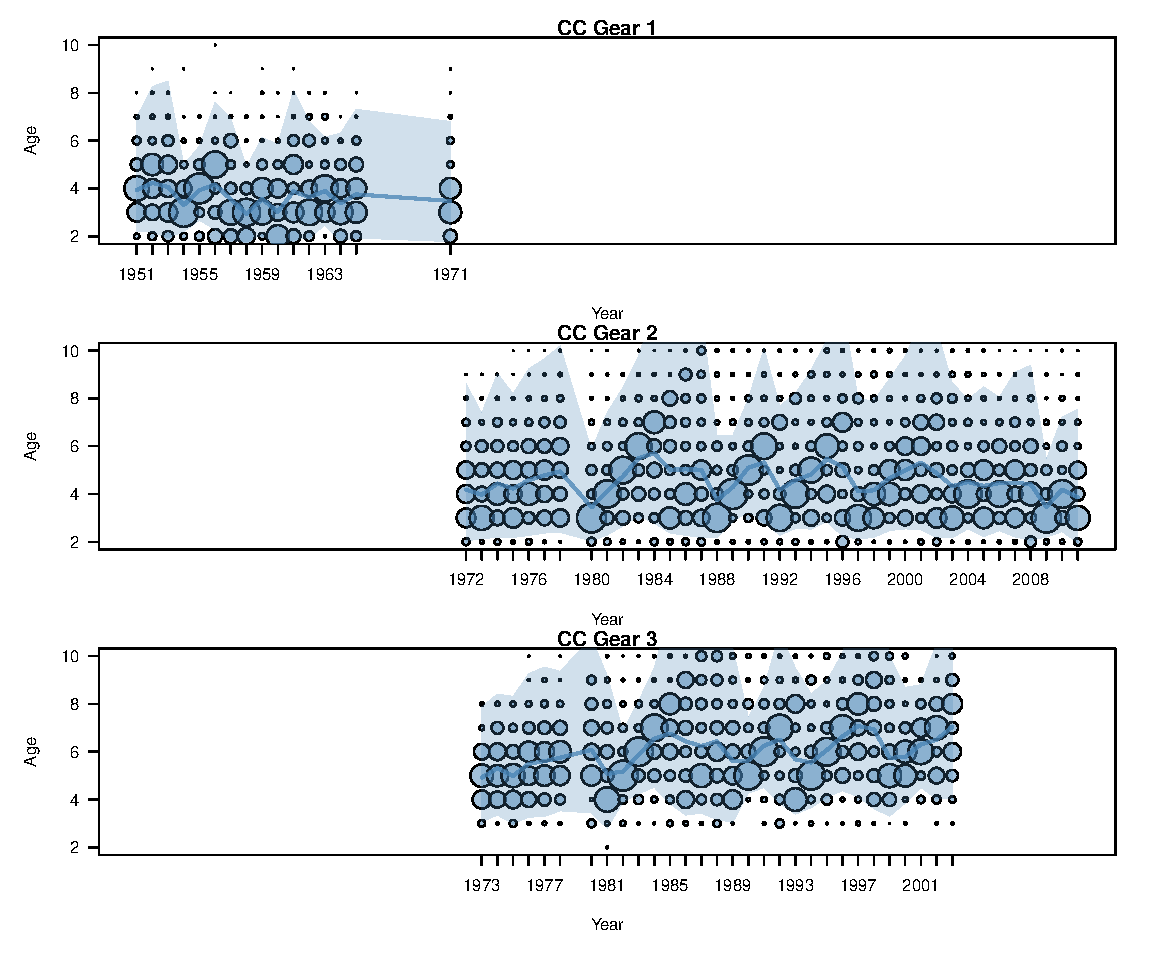
\includegraphics[width=0.85\textwidth]{../Figs/iscam_fig_AgeCompsCC.pdf}\\
	\caption{Bubble plots showing the proportions-at-age versus time for the winter purse seine fishery (top), seine roe fishery (middle) and the gillnet fishery (bottom) in the Central Coast region.  The area of the circle is proportional to cohort abundance, each column sums to 1, zeros are not shown, and age 10 is a plus group. Also shown is the mean age of the catch (line) and the approximate 95\% distribution of ages (shaded polygon) for each year.}\label{FigAgeCompsCC}
\end{sidewaysfigure}

\begin{sidewaysfigure}[!tbp]
	% Requires \usepackage{graphicx}
	\centering
	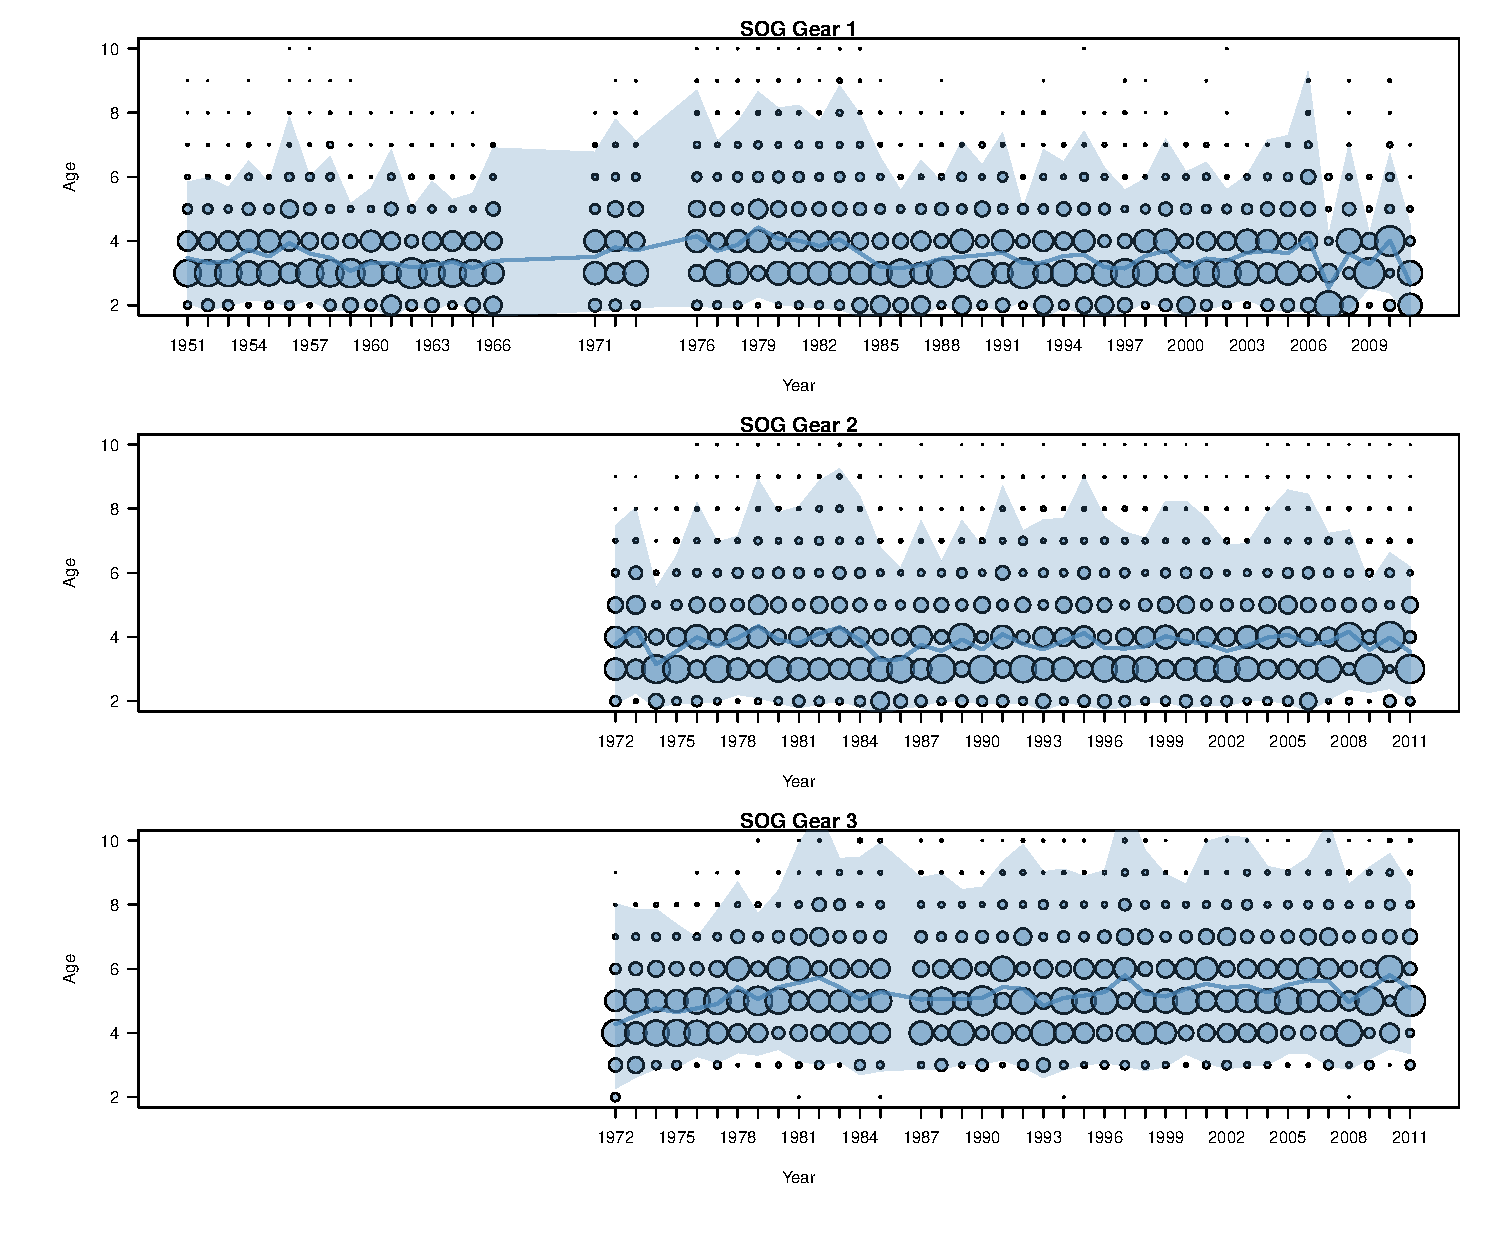
\includegraphics[width=0.85\textwidth]{../Figs/iscam_fig_AgeCompsSOG.pdf}\\
	\caption{Bubble plots showing the proportions-at-age versus time for the winter purse seine fishery (top), seine roe fishery (middle) and the gillnet fishery (bottom) in the Strait of Georgia.  The area of the circle is proportional to cohort abundance, each column sums to 1, zeros are not shown, and age 10 is a plus group. Also shown is the mean age of the catch (line) and the approximate 95\% distribution of ages (shaded polygon) for each year.}\label{FigAgeCompsSOG}
\end{sidewaysfigure}

\begin{sidewaysfigure}[!tbp]
	% Requires \usepackage{graphicx}
	\centering
	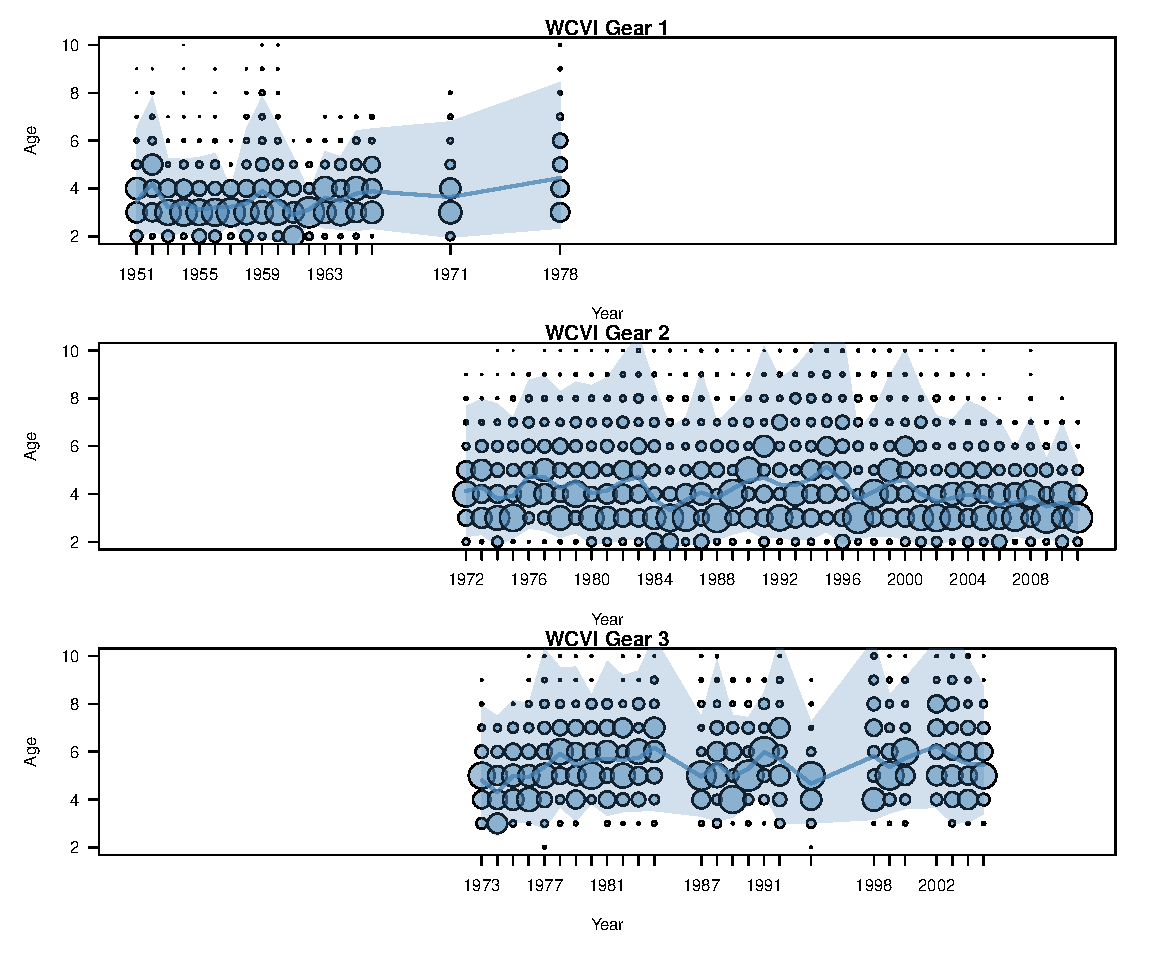
\includegraphics[width=0.85\textwidth]{../Figs/iscam_fig_AgeCompsWCVI.pdf}\\
	\caption{Bubble plots showing the proportions-at-age versus time for the winter purse seine fishery (top), seine roe fishery (middle) and the gillnet fishery (bottom) in the West Coast Vancouver Island region.  The area of the circle is proportional to cohort abundance, each column sums to 1, zeros are not shown, and age 10 is a plus group. Also shown is the mean age of the catch (line) and the approximate 95\% distribution of ages (shaded polygon) for each year.}\label{FigAgeCompsWCVI}
\end{sidewaysfigure}





	\subsubsection{Mean weight-at-age data}

	From the mid-1970s until the present, there has been a measurable decline in weight-at-age for all ages in all major stock areas (Figure \ref{FigMeanWt}). Samples collected during the 2009/10 fishing year indicate weights-at-age that are among the lowest on record. This declining weight-at-age may be attributed to any number of factors, including: fishing effects (i.e., gear selectivity), environmental effects (changes in ocean productivity), or it may even be attributed to changes in sampling protocols (shorter time frame over which samples are collected). Declining weight-at-age has been observed in all five of the major stocks, and despite area closures over the last 10-years, has continued to occur in the QCI and WCVI stocks. Although the direct cause of this decline is still to be investigated, this trend has been observed in B.C. and U.S. waters, from California to Alaska \citep{schweigert2002herring}, and merits further research.	The observed mean weight-at-age data appear to have a few  errors that need to be investigated as well; for example, see the apparently small age-10 fish in 2001 in Figure \ref{FigMeanWt}.

\begin{figure}[!tbp]
	% Requires \usepackage{graphicx}
	\centering
	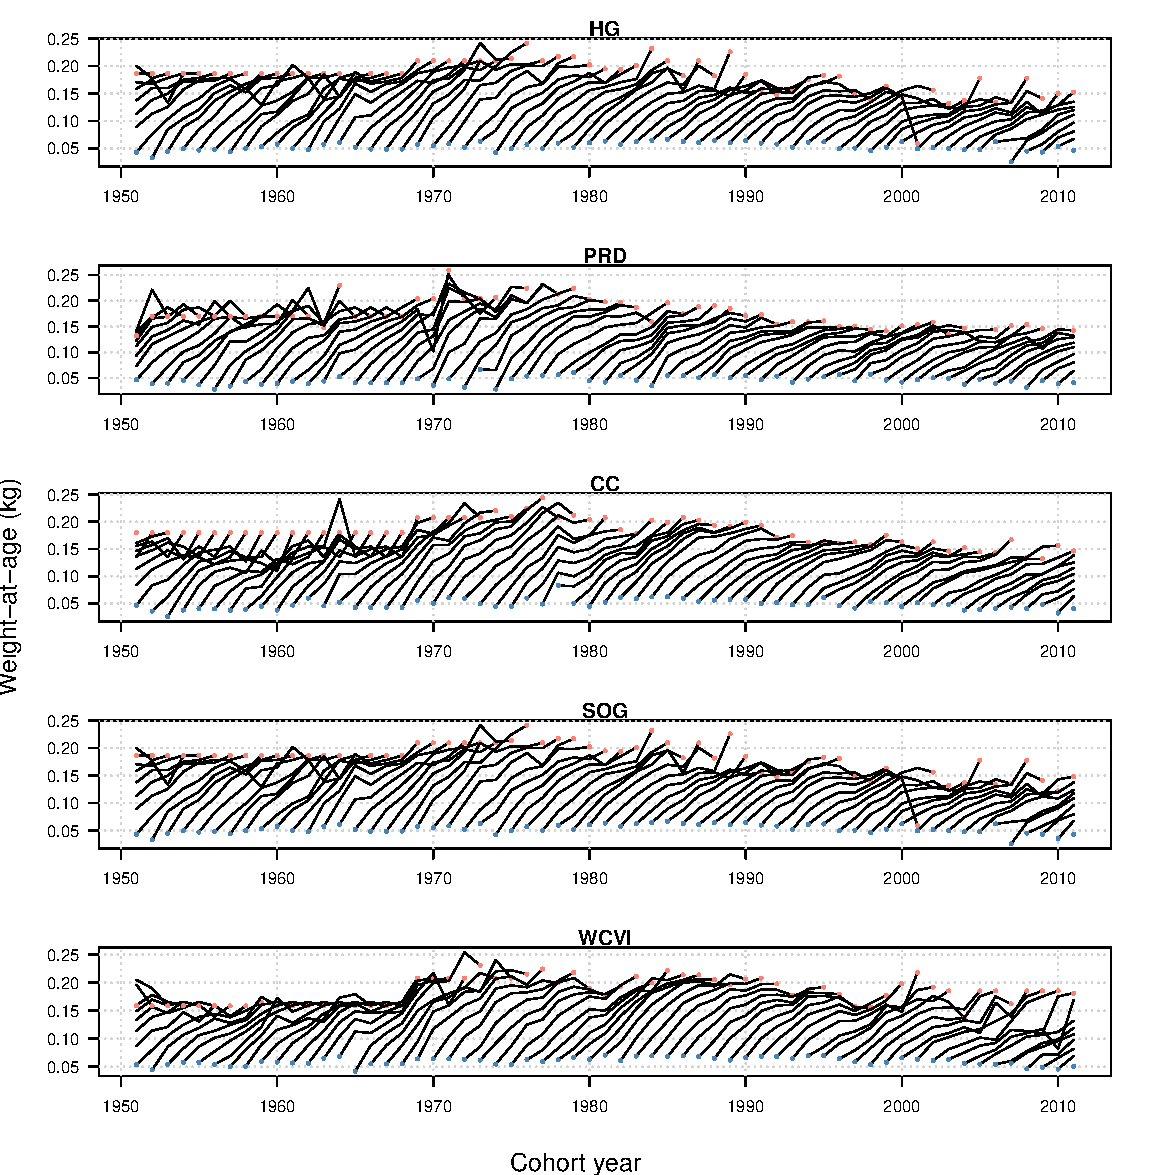
\includegraphics[width=\textwidth]{../Figs/iscam_fig_MeanWt.pdf}\\
	\caption{Empirical mean weight-at-age data by cohort from 1951 to 2011 for ages 2 to 10 in the five major Stock Assessment Regions.}\label{FigMeanWt}
\end{figure}
	

%%%%%%%%%%%%%%%%%%%%%%%%%%%%%%%%%%%%%%%%%%%%%%%%%%%%%%%%%%%%%%%%%%%%%
%%%%%%%%%%%%%%%%%%%%%%%%%%%%%%%%%%%%%%%%%%%%%%%%%%%%%%%%%%%%%%%%%%%%%
%%%%%%%%%%%%%%%%%%%%%%%%%%%%%%%%%%%%%%%%%%%%%%%%%%%%%%%%%%%%%%%%%%%%%	
	\subsection{Analytical methods}

	For the 2011 BC herring assessment, \iscam was used to conduct the stock assessment for each of the five major Stock Assessment Regions (SAR) and two minor assessment areas (Area 2W and Area 27).  The technical details of this model can be found in Appendix \ref{appiSCAM}.
		
	\subsection{Retrospective analysis}
	A retrospective analysis was conducted for each of the major and minor SARs.  The retrospective analysis successively removes the last 10-years of data and examines changes in estimates of terminal spawning biomass.  The results are then plotted on a single panel to compare how estimates of spawning biomass change as successive years of data are omitted from the analysis.
	
	\subsection{Abundance and recruitment forecasts}
	The abundance forecast for the upcoming fishing season, also referred to as pre-fishery biomass, is defined as the predicted biomass of age-4 fish and older plus the number of age-3 fish recruiting in year $T+1$.  The abundance estimates are based on the median values from the sampled posterior distribution.  Age-3 recruits are based on poor, average, and good recruitment scenarios; see next paragraph for definitions of poor, average and good.
	
	The recruitment forecasts are based on the surviving number of age-3 fish at the start of the fishing season times the average weight-at-age 3 in the last 5 years. The definitions of poor, average, and good recruitment are as follows: \textbf{Poor} is the average recruitment from the 0-33 percentile, \textbf{Average} is the average recruitment from the 33-66 percentile, and \textbf{Good} is the average recruitment from the 66-100 percentile.  Note that all cohorts from 1951 to 2011  were included in the calculation of recruitment quantiles.
	
	\subsection{Catch advice}
Catch advice is based on the application of the harvest control rule (HCR). The herring HCR has three components:
\begin{enumerate}
\item Reference points (LRP, USR, and cuttoffs)
\item Harvest rate
\item Decision rules
\end{enumerate}

For each of the five major stocks, the limit reference point (LRP) is the cuttoff value, which is defined here as 0.25\bo\, and the	Upper Stock Reference (USR) is defined as the 1.05*LRP (0.25\bo\ + 0.2*0.25\bo = LRP + 0.05LRP). \textbf{For clarification, references to \bo\ throughout this document refer to the mature spawning stock biomass.} The default harvest rate if the stock is at or above USR is 0.2, and declines linearly to 0 when the stock is at or below the LRP (a default harvest rate of 0.1 is used for the minor stock areas).  The decision rule for the major stock areas operates as follows:

\begin{itemize}
	\item If the forecast run is less than the LRP (cuttoff) then the area is closed to all commercial harvest  (i.e., stock is deemed to be in the critical zone).
	
	\item If the forecast run is greater than the LRP and less than the USR (i.e., cautious zone), then total allowable catch is based on a reduced harvest rate that would deplete the stock to the LRP level.
	
	\item If the forecast run is greater than USR, then the total allowable catch is set at 20\% of the forecast run.
\end{itemize}



	

%    %!TEX root = /Users/stevenmartell/Documents/CURRENT PROJECTS/iSCAM-trunk/fba/BC-herring-2011/WRITEUP/BCHerring2011.tex
\section{Results}
The results section is broken down into three major subsections, Maximum likelihood fits to the data, marginal posterior distributions, and stock forecasts and catch advice based on samples from the joint posterior distribution.

\subsection{Maximum likelihood fits to the data}
Although  the maximum likelihood estimates are not explicitly used for constructing the catch advice, we do present the MLE estimates of the residual patterns and fits to the data for comparisons.

\subsubsection{Catch residuals}
Residuals between the observed and predicted catch are largely determined by the user specified standard deviation in each of the control files.  In this assessment, the assumed variance for all regions (including minor regions) was set at 0.005, which corresponds to a standard deviation of approximately 0.0707.  Overall the residuals for each fishery in each stock assessment region are unremarkable (Fig. \ref{PartII:Results:fig1}), with exception of a  major outlier in the Haida Gwaii in the mide 1950s.  In 1956, the reported catch in Haida Gwaii was extremely large ($>$ 60,000 mt) and the model has a difficult time explaining this large catch. In order to explain this large catch in a single year, a large biomass in the region is required.

\begin{figure}[!tbp]
	% Requires \usepackage{graphicx}
	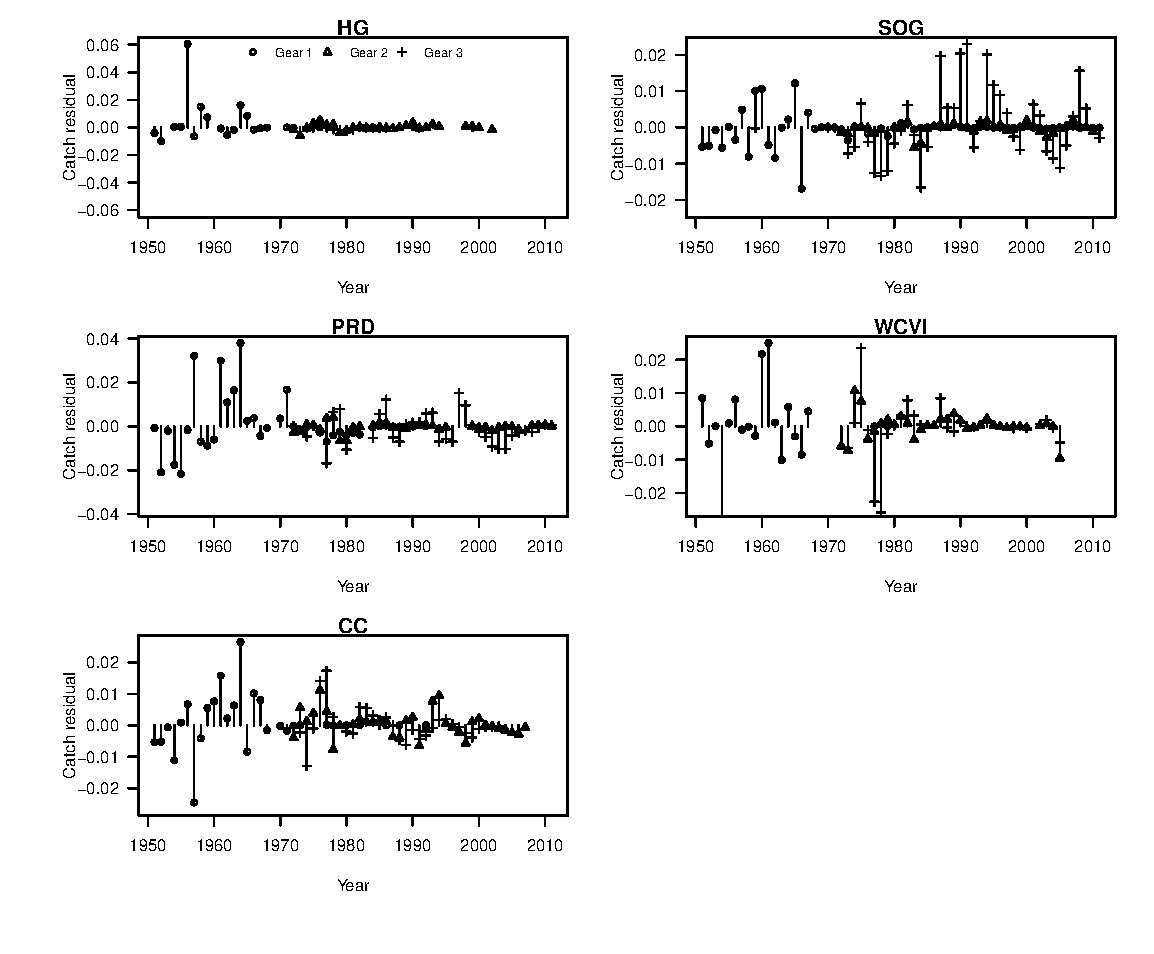
\includegraphics[width=\textwidth]{../FIGS/qPriorFigs/iscam_fig_catchresid.pdf}\\
	\caption{Residual for the log difference between observed and predicted catch for the five major SARs for each gear type (Gear 1 = winter seine fishery, Gear 2 = seine-roe fishery, Gear 3 = gill net fishery).}\label{PartII:Results:fig1}
\end{figure}


\subsubsection{Fits to the spawn survey data}
The residuals between the observed and predicted spawn survey index (on a log scale) are shown in Figure \ref{PartII:Results:fig2}.  Recall that the spawn survey data are treated as two independent time series where data between 1951--1987 were based on surface estimates of spawn area and data post 1988 are based on diver surveys of spawn area.  More weight was assigned to the contemporary data.   

For most areas, there is little pattern in the residuals between the observed and predicted survey data (Fig \ref{PartII:Results:fig2}).  For the HG, PRD and CC regions, there is very good correspondence between the observed and predicted survey data post 1988.  IN the SOG, there is a period of positive residuals between 1999 and 2005 where the predicted spawn biomass fails to increase as much as indicated by the survey.  Similary 3--4 year trends also exist in the WCVI spawn survey data after the year 2000.

\begin{figure}[!tbp]
	% Requires \usepackage{graphicx}
	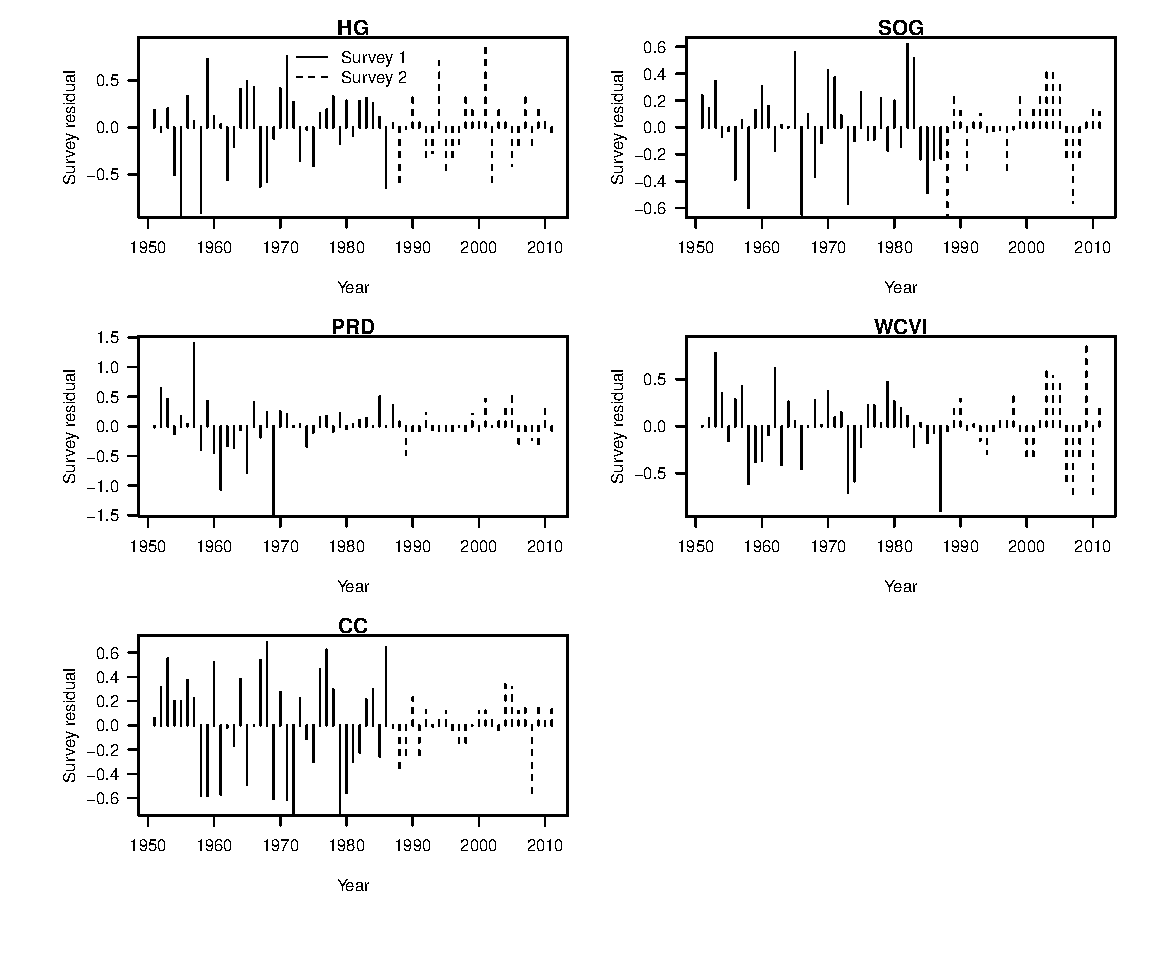
\includegraphics[width=\textwidth]{../FIGS/qPriorFigs/iscam_fig_surveyresid.pdf}\\
	\caption{Residual patterns for the log difference between observed and predicted spawn survey abundance for the five major SARs. Spawn survey data based on surface estimates are show as solid lines and data based on diver surveys is shown as dashed lines.}\label{PartII:Results:fig2}
\end{figure}

In comparison to the previous assessment for Pacific herring using the HCAM model, estimates of the catchability coefficient are very different (HCAM assumed q=1 for post 1988 data).  In each of the five major assessment regions (and the two minor regions) a less informative prior for the catchability coefficient was used (see Appendix \ref{Appendix::q_prior}).  Maximum Likelihood Estimates (MLE) of the catchability coefficients are presented for each region in Fig. \ref{PartII:Results:fig3} along with the observed and predicted trends in the spawn index.  Estimates of $q$ in both time periods are less than 1.0 for all regions with the exception of post 1988 data in the PRD region.  The interpretation of $q=1$ is that the spawn survey data is an absolute measure of spawn abundance, $q<1$ implies that the survey under-estimates the spawn abundance and $q>1$ implies an over-estimate.  For example, in the HG region the MLE values for $q$ are 0.245 and 0.433 for the pre- and post-1988 data, respectively. This could be interpreted as the spawn survey only, on average, sees 24.5\% and 43.3\% of the deposited spawn each year.  This interpretation however is conditional on the specification of mature biomass in the stock assessment model. 

\begin{figure}[!tbp]
	% Requires \usepackage{graphicx}
	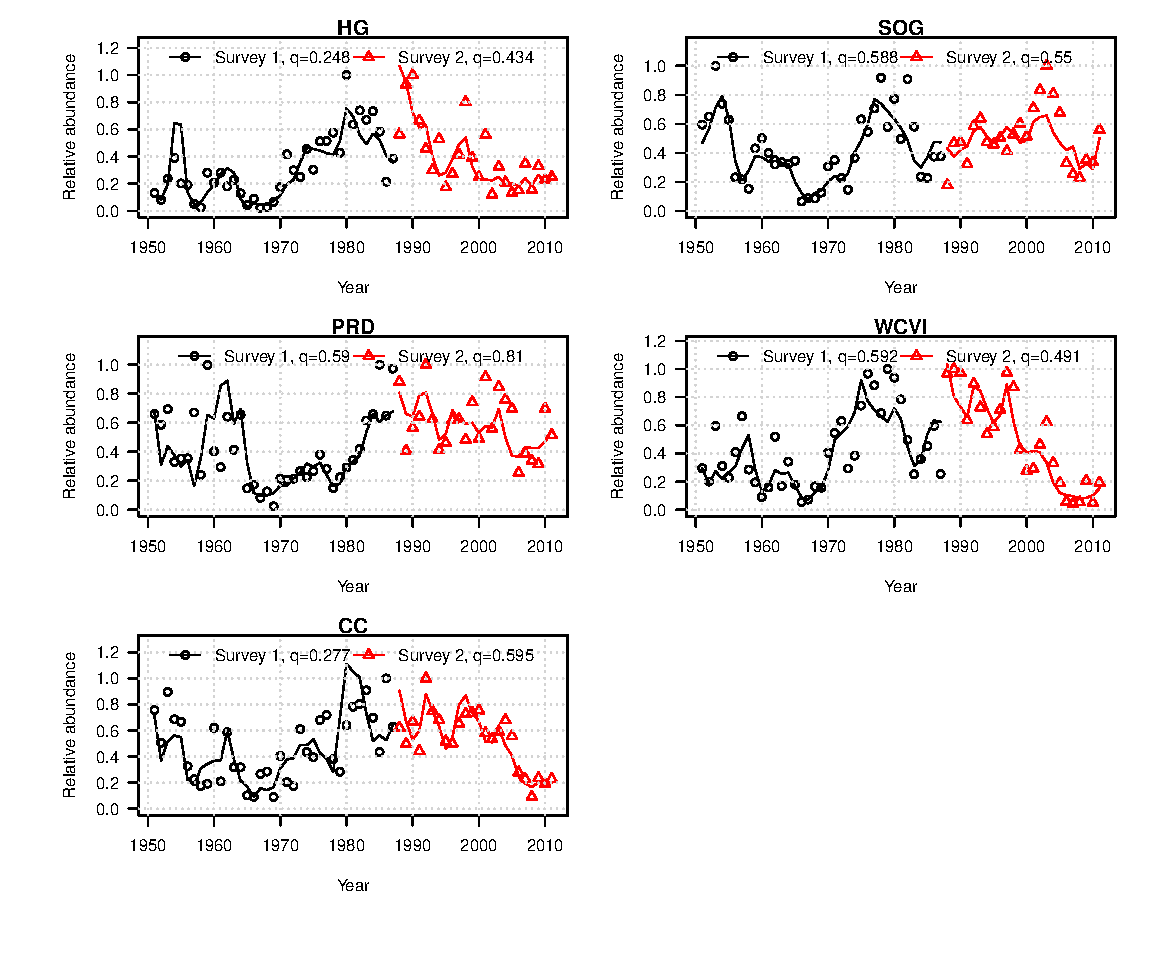
\includegraphics[width=\textwidth]{../FIGS/qPriorFigs/iscam_fig_surveyfit.pdf}\\
	\caption{Observed (points) and predicted (lines) relative abundance data (spawn survey data) for each of the five major SARs.  In each panel, the corresponding scaler ($q$) is presented for each of the surveys.}\label{PartII:Results:fig3}
\end{figure}


\subsubsection{Age composition residuals}

The assumed error distribution for the age-composition data has changed in this assessment from a multinomial distribution implemented in HCAM to a multivariate-logistic distribution. In the former implementation the age-composition data were weighted by the annual samples sizes in each region for each age and year. In the \iscam\ implementation the age-composition data for all years is given the same weight (i.e., we assume the observation errors is homogenous) based on the conditional maximum likelihood estimate of the variance (see Appendix \ref{appiSCAM} for full details).  We further pool age-proportions that are less than 2\% into the adjacent younger year class to reduce the influence of small outliers and weak cohorts.

In HG the MLE estimates of the variance for each gear is 0.102, 0.104 and 0.351, for the winter seine, seine-roe and gill net fleets, respectively (Fig. \ref{PartII:Results:figAgeCompHG}).  In general there is fairly good agreement between the observed and predicted age-composition data in this region, with poorer fits to the gill net age-composition data.  There is no persistent pattern in the residuals. 

\begin{sidewaysfigure}[!tbp]
	% Requires \usepackage{graphicx}
	\centering
	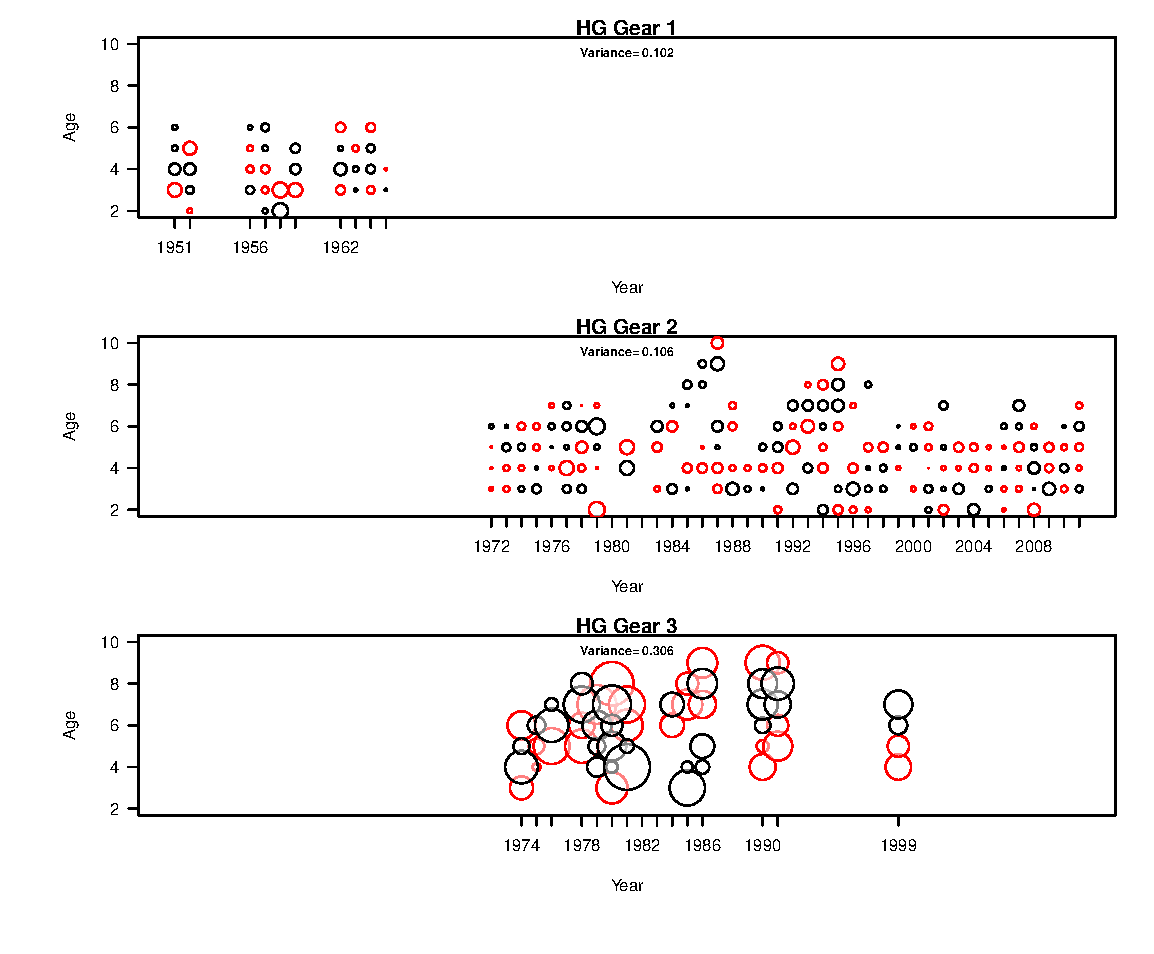
\includegraphics[width=0.9\textwidth]{../FIGS/qPriorFigs/iscam_fig_agecompsresid_HG.pdf}\\
	\caption{Residual difference between the observed and predicted proportions-at-age for HG for each of the three gear types (Gear 1 = winter seine, Gear 2 = seine-roe, Gear 3 = gill net).  The area of each circle is proportional to the residua, black is positive, and red is negative.  The corresponding MLE estimates of the residual variance is displayed in each panel.}\label{PartII:Results:figAgeCompHG}
\end{sidewaysfigure}

For the PRD region, the fits to the age-composition data are slightly poorer, with MLE estimates of the variance ranging from 0.215 to 0.358 for the seine-roe and gill net fleets (Fig. \ref{PartII:Results:figAgeCompPRD}). There is no remarkable pattern in the winter seine fishery, the seine-roe fishery tends to have positive residuals for age-3 and age 7+ fish, and negative residuals for ages 4-6 fish.  Similarly, the is an age-pattern in the residuals for the gill net fishery with negative residuals for age-4 and ages 9+ fish, and positive residuals for ages 5-8.  Residuals in 2011 age-composition data are much larger  than all other years.

\begin{sidewaysfigure}[!tbp]
	% Requires \usepackage{graphicx}
	\centering
	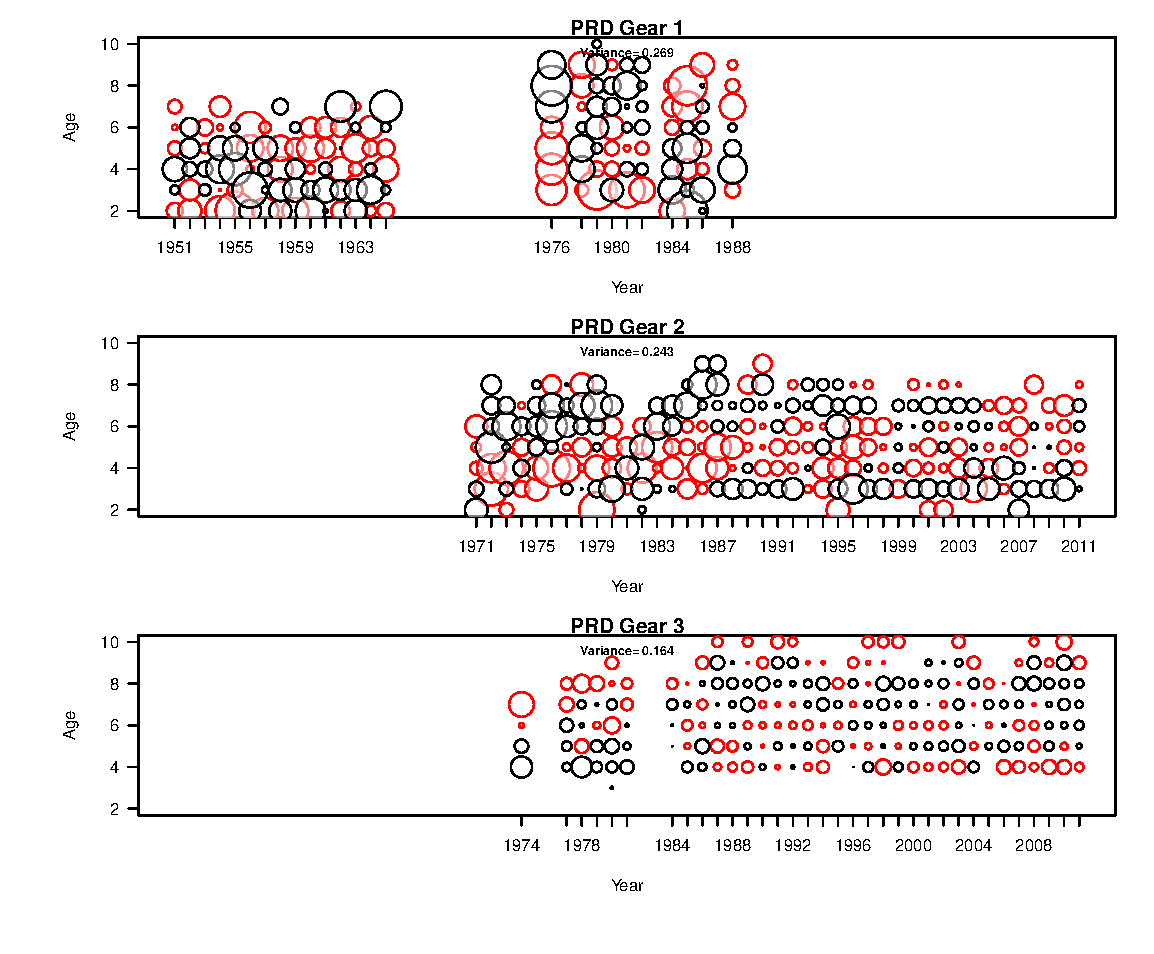
\includegraphics[width=0.9\textwidth]{../FIGS/qPriorFigs/iscam_fig_agecompsresid_PRD.pdf}\\
	\caption{Residual difference between the observed and predicted proportions-at-age for PRD for each of the three gear types (Gear 1 = winter seine, Gear 2 = seine-roe, Gear 3 = gill net).  The area of each circle is proportional to the residua, black is positive, and red is negative.  The corresponding MLE estimates of the residual variance is displayed in each panel.}\label{PartII:Results:figAgeCompPRD}
\end{sidewaysfigure}


For the Central Coast (CC) region, there is also good correspondence between the observed and predicted age-composition data, with MLE estimates of the variance ranging from 0.128 to 0.203 (Fig. \ref{PartII:Results:figAgeCompCC}).  There is no striking temporal pattern in the residuals for any of the fishing fleets.  There is a tendency to overestimate the porportion-at-age 4 and 5 in the seine-roe fishery.


\begin{sidewaysfigure}[!tbp]
	% Requires \usepackage{graphicx}
	\centering
	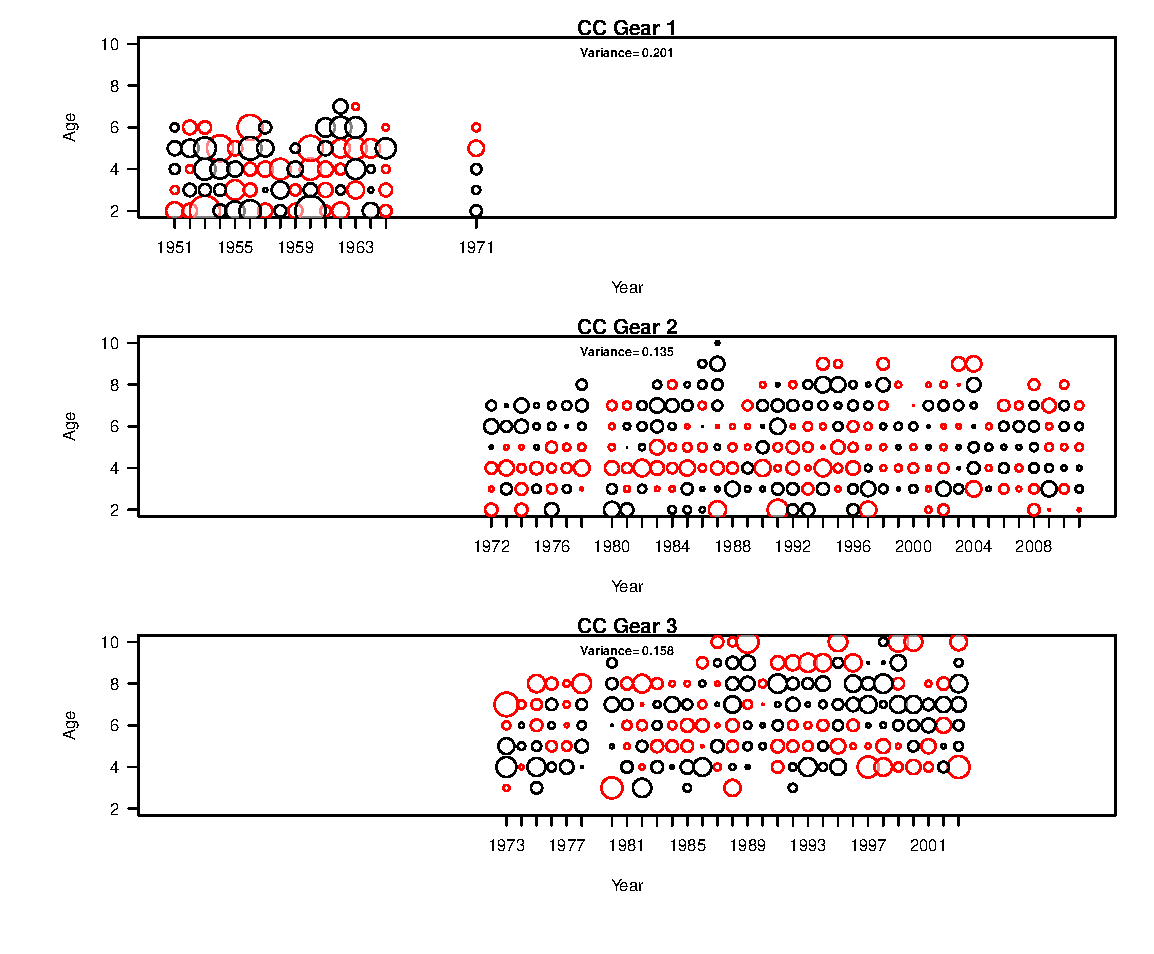
\includegraphics[width=0.9\textwidth]{../FIGS/qPriorFigs/iscam_fig_agecompsresid_CC.pdf}\\
	\caption{Residual difference between the observed and predicted proportions-at-age for CC for each of the three gear types (Gear 1 = winter seine, Gear 2 = seine-roe, Gear 3 = gill net).  The area of each circle is proportional to the residua, black is positive, and red is negative.  The corresponding MLE estimates of the residual variance is displayed in each panel.}\label{PartII:Results:figAgeCompCC}
\end{sidewaysfigure}

For the Strait of Georgia, there is also very good correspondence between the observed and predicated age-composition data for all three gears (Fig \ref{PartII:Results:figAgeCompSOG}).  The MLE estimates of the variance range from 0.088 to 0.021 for the seine-roe and gill net fleets, respectively.  In the gill net fleet  there has been a tendency to under-estimate the proportions-at-age 4-6 between the 1970s and mid 1990s and more recently to over-estimate the proportions-at-age 6-8.  Recall that selectivity for the gill net fishery is a function of the empirical weight-at-age data, which has been trending to small fish in recent years.


\begin{sidewaysfigure}[!tbp]
	% Requires \usepackage{graphicx}
	\centering
	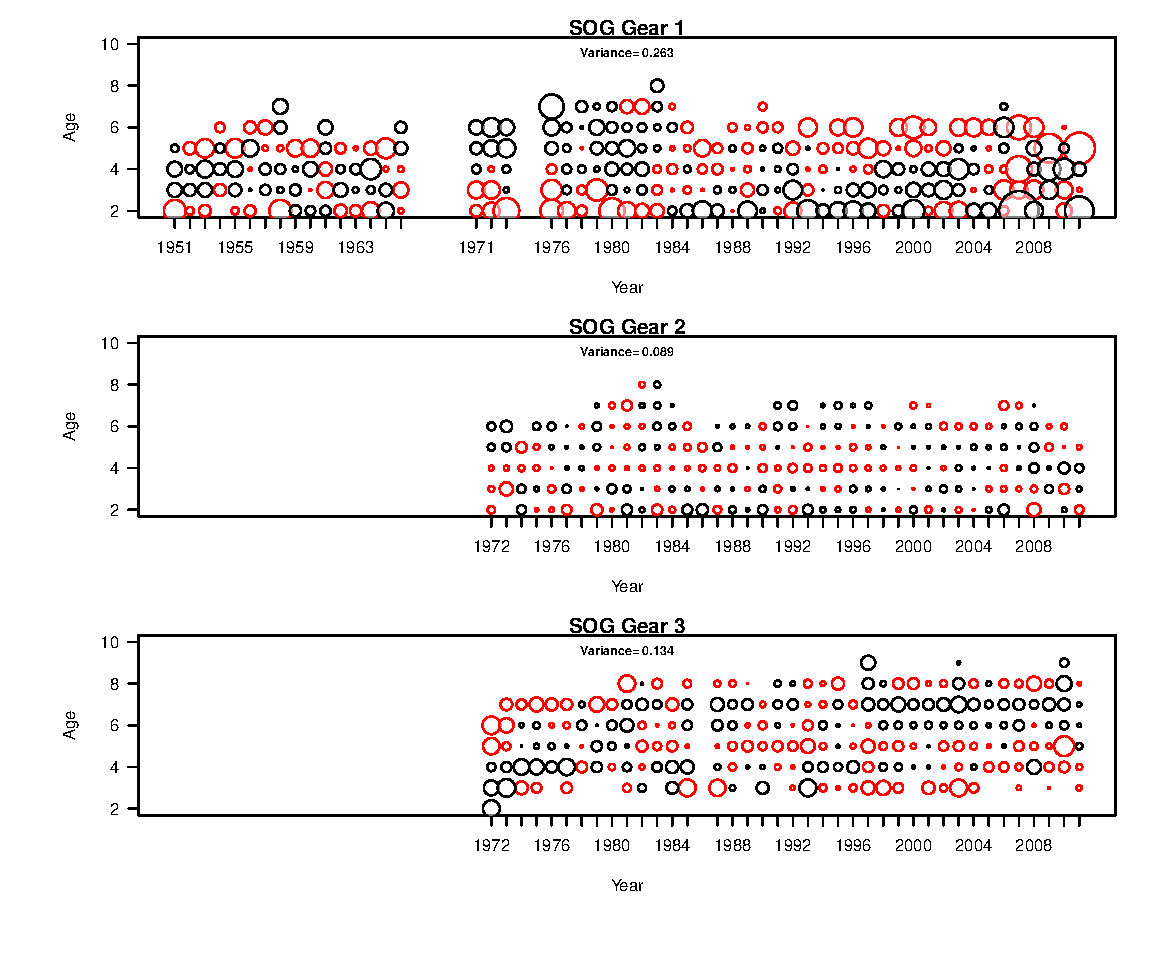
\includegraphics[width=0.9\textwidth]{../FIGS/qPriorFigs/iscam_fig_agecompsresid_SOG.pdf}\\
	\caption{Residual difference between the observed and predicted proportions-at-age for SOG for each of the three gear types (Gear 1 = winter seine, Gear 2 = seine-roe, Gear 3 = gill net).  The area of each circle is proportional to the residua, black is positive, and red is negative.  The corresponding MLE estimates of the residual variance is displayed in each panel.}\label{PartII:Results:figAgeCompSOG}
\end{sidewaysfigure}

In the case of WCVI, there is good correspondence between the observed and predicted age composition data for the seine fisheries and less so for the gill net fishery (Fig \ref{PartII:Results:figAgeCompWCVI}).  The MLE estimates of the variance range fro 0.088 to 0.314 for the seine-roe and gill net fisheries, respectively.  Residual patterns in the seine fisheries are unremarkable, perhaps an age-pattern in the seine roe fishery.  There is a tendency to under-estimate the proportions-at-age in the gill net fishery for ages 5-7.   The size of the residuals are fairly homogenous over time for all gears.


\begin{sidewaysfigure}[!tbp]
	% Requires \usepackage{graphicx}
	\centering
	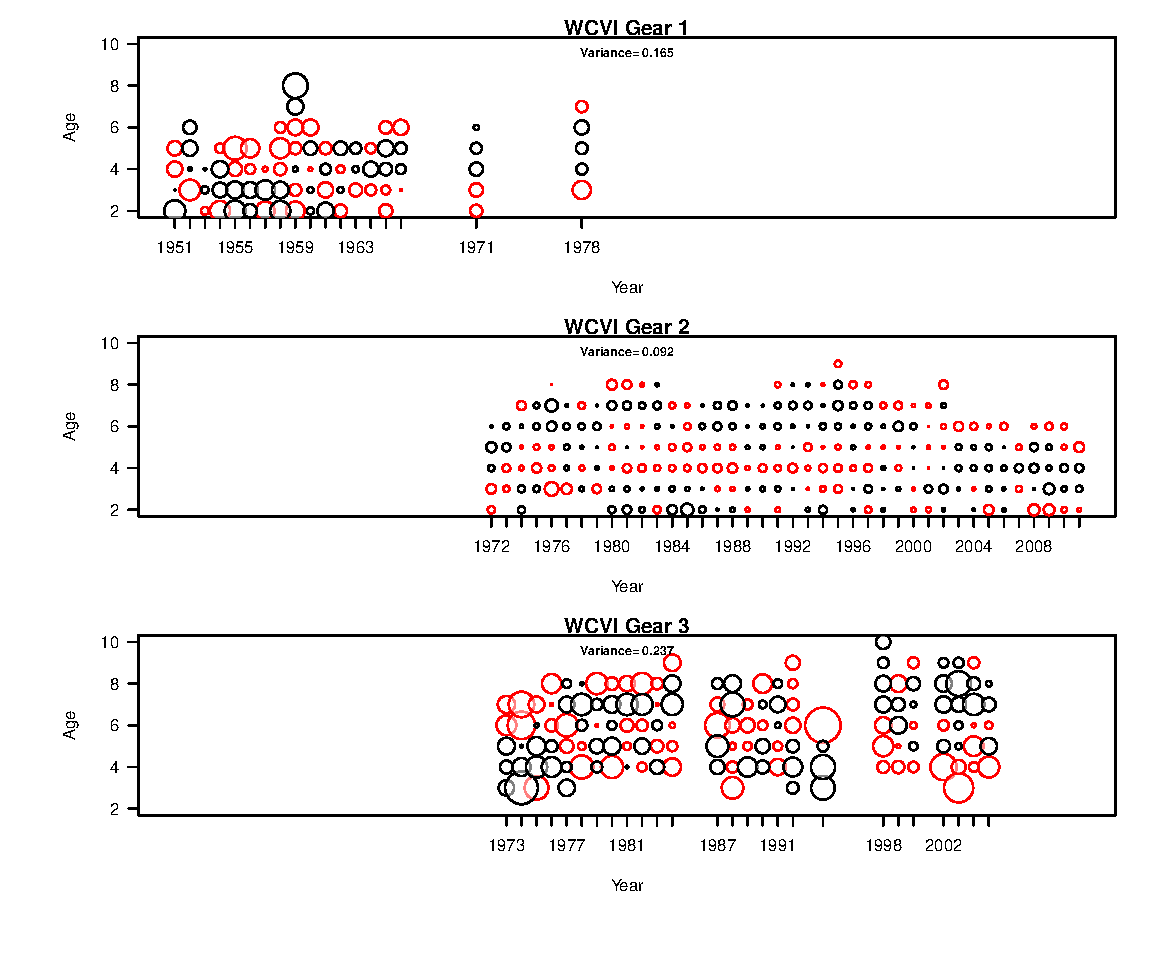
\includegraphics[width=0.9\textwidth]{../FIGS/qPriorFigs/iscam_fig_agecompsresid_WCVI.pdf}\\
	\caption{Residual difference between the observed and predicted proportions-at-age for WCVI for each of the three gear types (Gear 1 = winter seine, Gear 2 = seine-roe, Gear 3 = gill net).  The area of each circle is proportional to the residua, black is positive, and red is negative.  The corresponding MLE estimates of the residual variance is displayed in each panel.}\label{PartII:Results:figAgeCompWCVI}
\end{sidewaysfigure}







\subsubsection{Biomass estimates \& reference points}

Maximum likelihood estimates of total biomass (age 2+) and the spawning stock biomass for each of the five major assessment regions in summarized in Figure \ref{PartII:Results:figBiomass}.  Estimates of spawning stock depletion ($B_t/B_0$) for the five major regions is summarized in Figure \ref{PartII:Results:figDepletion} along with estimates of the sustainable fisheries framework reference points.  With the exception of the SOG, estimates of spawning stock depletion in 2011 are all currently below 40\% of their estimated unfished state, and in PRD, CC and the WCVI  are all estimated to be below 25\% of their unfished state (Fig \ref{PartII:Results:figDepletion}).

Spawning stock biomass in 2011 was estimated as follows: HG -- 16,789 tonnes, PRD -- 18,170 tonnes, CC -- 11,077 tonnes, SOG -- 72,135 tonnes, and WCVI -- 11,764 tonnes (Table \ref{PartII:Table1:referencePoints}).  With the exception of the PRD, these estimates are considerably higher in comparison to last years HCAM estimates; the difference largely owes to the substantial change in spawn survey scaling coefficient ($q$).

In addition to the current estimates of spawning biomass, Table \ref{PartII:Table1:referencePoints} also summarizes estimates of reference points and the total number of estimated parameters for each of the five major stock assessment regions.  Each region contained data from 1951 to 2010, and the number of estimated parameters ranges from 158 in HG to 234 in SOG.  The difference in the number of estimated parameters owes to the difference in the number of years of catch data for each region.

Estimates of unfished spawning biomass for each region is as follows: HG -- 40,960 tonnes, PRD -- 80,247 tonnes, CC -- 56,181 tonnes, SOG --- 116,023 tonnes, and WCVI -- 51,379 tonnes.  Applying the same cuttoff rule used in previous assessments (25\% of $B_0$), the results in a substantial change in the cuttoff levels for PRD, CC, SOG, and WCVI.  The previous cuttoff level for HW was estimated at 10,700 tonnes, and in this assessment there is a minor downward revision to 10,240 tonnes.  In the case of PRD, the previous cuttoff was 12,100 tonnes and in this assessment is now 20,062 tonnes.  For the CC, the previous cuttoff was 17,600 tonnes and now 14,045 tonnes.  For the SOG, the previous cuttoff was 21,200 tonnes, and in this assessment it has been revised upwards to 29,006 tonnes.  Lastly, for the WCVI the cuttoff has decreased from 18,800 tonnes to 12,845 tonnes.


% latex.default(rpTable, file = fn, title = "Stock", longtable = FALSE,      landscape = FALSE, cgroup = NULL, n.cgroup = NULL, caption = cap,      label = "TableRefPoints", na.blank = TRUE, vbar = FALSE,      size = "small") 
%
\begin{table}[!tbp]
 \small
 \caption{Summary of maximum likelihood estimates for  the 
	two minor stock areas.  No. is the total number of estimated 
	parameters, \fmsy\ the average instantaneous fishing rate to 
	achieve the maximum sustainable yield (MSY), \bo\ is the unfished 
	spawning biomass, \bmsy\ is the spawning biomass that achieves 
	maximum sustainable yield,$B_t$ is the spawning biomass at the end 
	of the 2011 fishing season, and $B_t/B_0$ is the spawning depletion 
	level at the end of the 2011 fishing season.\label{TableRefPoints}} 
 \begin{center}
 \begin{tabular}{lll}\hline\hline
\multicolumn{1}{l}{Stock}&\multicolumn{1}{c}{A2W}&\multicolumn{1}{c}{A27}\tabularnewline
\hline
No.&74&79\tabularnewline
\fmsy& 0.34&  1.9\tabularnewline
MSY&  265&  304\tabularnewline
$B_0$&2,915&2,084\tabularnewline
0.25$B_0$&  729&  521\tabularnewline
\bmsy&  705&  447\tabularnewline
0.8\bmsy&  564&  358\tabularnewline
0.4\bmsy&  282&  179\tabularnewline
$B_t$&4,671&  924\tabularnewline
$B_t/B_0$&  1.6& 0.44\tabularnewline
\hline
\end{tabular}

\end{center}

\end{table}




\begin{figure}[!tbp]
	% Requires \usepackage{graphicx}
	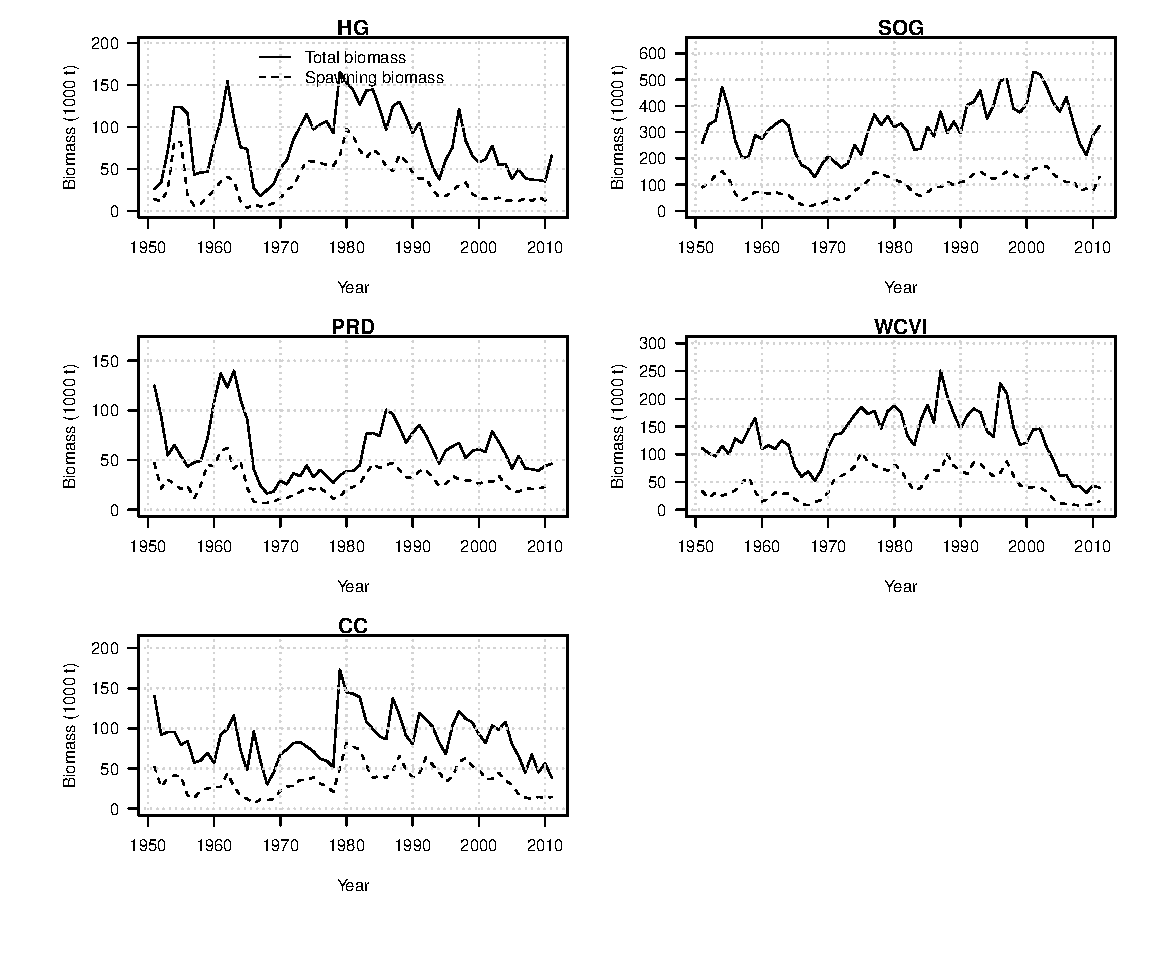
\includegraphics[width=\textwidth]{../FIGS/qPriorFigs/iscam_fig_biomass.pdf}\\
	\caption{Estimates of total biomass at the start of the year (numbers times empirical weight-at-age) and spawning stock biomass (post fishery) for the five major SARs.}\label{PartII:Results:figBiomass}
\end{figure}


\begin{figure}[!tbp]
	% Requires \usepackage{graphicx}
	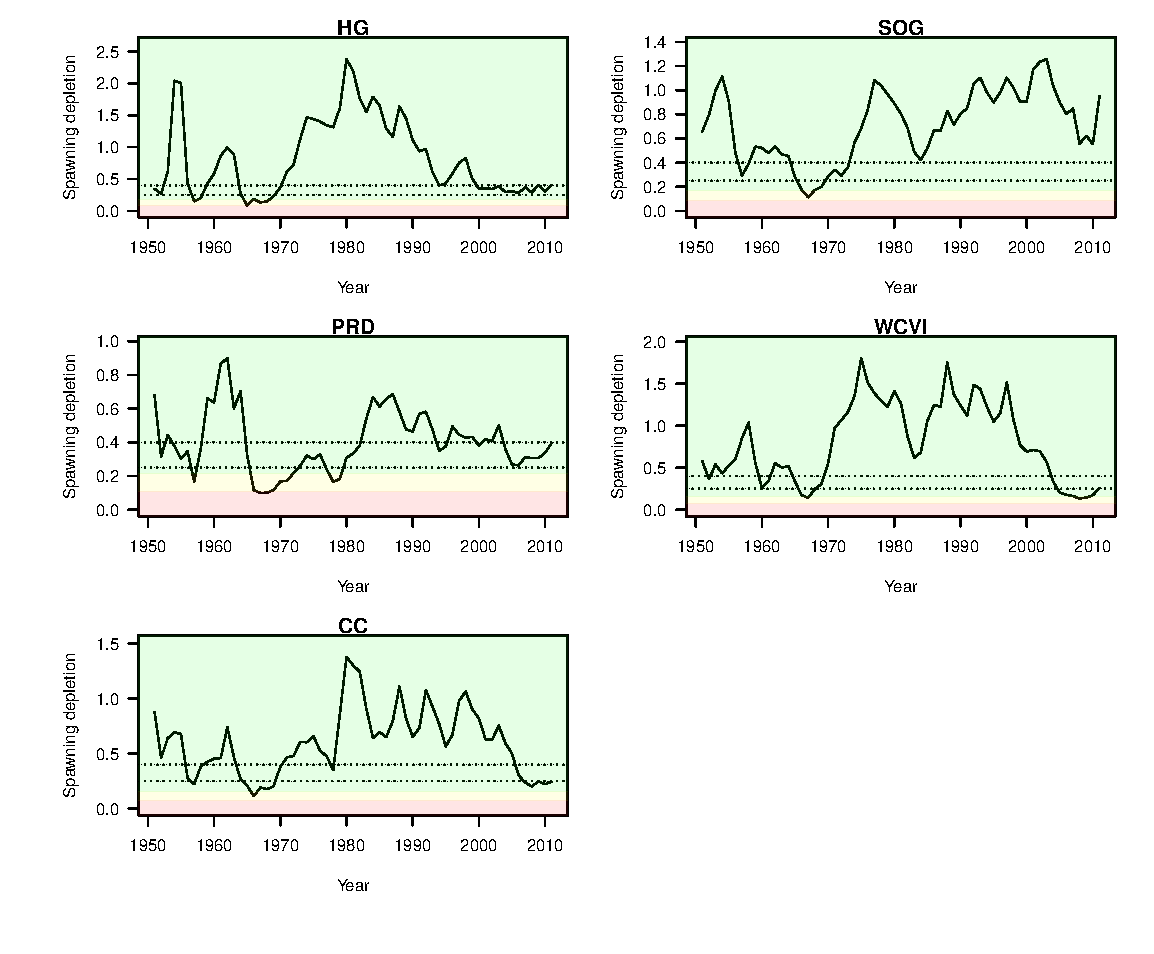
\includegraphics[width=\textwidth]{../FIGS/qPriorFigs/iscam_fig_depletion.pdf}\\
	\caption{Estimates of spawning biomass depletion ($B_t/B_0$) for each of the five major stock areas.  Horizontal dotted lines represent 25\% and 40\% depletion levels, and the shaded regions demarcate reference points based on $<$40\% \bmsy/\bo (critical zone) and 40--80\% \bmsy/\bo(cautious zone) and $>$80\% \bmsy/\bo (healthy zone).}\label{PartII:Results:figDepletion}
\end{figure}




\subsubsection{Estimates of mortality}

The most recent HCAM assessment model allowed for annual estimates of $M_t$ where natural mortality was modelled as a random walk process.  The same random walk model has been adopted in this \iscam\ implementation, however, a reduced number of parameters (12 nodes instead of 60 annual deviations) is estimated and interpolated using a bicubic spline.  The number of estimated nodes does have minor influences on the various trends in natural mortality; we came to arrive at estimating 12 nodes by ensuring the estimated trends were very similar to trends in $M$ when estimated annual natural mortality rates (NB. one could use formal model selection criterion here to determine the optimal number of nodes).

For all of the five major stock assessment regions, estimates of natural mortality rates have trended upwards since the 1950s (Figure \ref{PartII:Results:figMortality}).  Trends in estimates of natural mortality are also consistent with the trends in natural mortality from last years HCAM model  \citep[see Figure 18 in][]{Clear2010}.  In the mid to late 1970s, estimates of natural mortality rates were very low during a time when most of the stocks were recovering from the earlier reduction fishery.  In the last decade, estimates of natural mortality rates for herring have been at an all time high, and in some locations (HG, CC SOG and WCVI) there is indication that natural mortality rates may be declining. Estimates of $M_t$ in the most recent years, however,  are highly suspect because there are incomplete cohorts to infer estimates of total mortality rates.



\begin{figure}[!tbp]
	% Requires \usepackage{graphicx}
	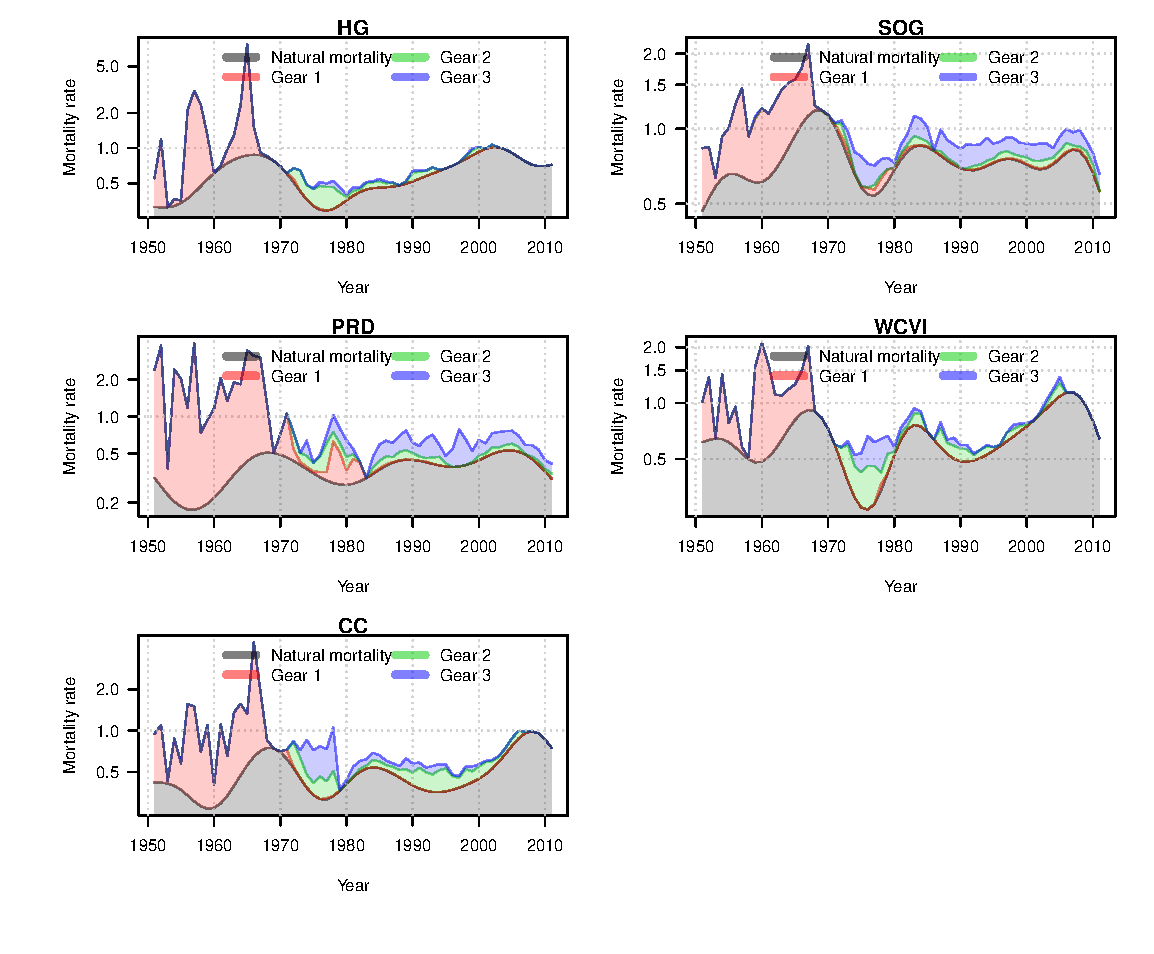
\includegraphics[width=\textwidth]{../FIGS/qPriorFigs/iscam_fig_mortality.pdf}\\
	\caption{Maximum likelihood estimates of the components of average total mortality for each of the five major stock assessment regions. Note that the y-axis is plotted on a log scale, natural mortality (grey) is age-independent, fishing mortality is age-specific and the average fishing mortality rate over all age-classes is plotted here.}\label{PartII:Results:figMortality}
\end{figure}

Estimates of fishing mortality rates in each of the regions, between 1951 and 1970 were very high due to the purse-seine fleet during the reduction fishery.  After the fishery re-opened in the early 1970s fishing mortality rates have been greatly reduced and periodic since the early 1990s due to the cuttoffs.  Of notable exception is the fishing mortality rate for the gill net fishery in PRD in the late 2000s (Fig. \ref{PartII:Results:figMortality}). This appears to be an artifact due to the structural assumption that selectivity is a function of weight-at-age.  Estimates of selectivity for the gill net fleet are all much less than 1 due to the small size of herring in the PRD region in the 2000s.

\subsubsection{Selectivity}

\subsubsection{Recruitment and stock-recruitment relationships}


\subsection{Marginal posterior distributions}

\subsection{Forecast and catch advice based on the joint posterior distribtution}
 The catch advice in Tables \ref{TableCatchAdvice} and \ref{TableCatchAdviceqFix} is based on the old cuttoffs.


% latex.default(xTable, file = fn, rowname = NULL, longtable = FALSE,      landscape = FALSE, cgroup = cgrp, n.cgroup = ncgrp, caption = cap,      label = "TableCatchAdvice", na.blank = TRUE, vbar = FALSE,      size = "small") 
%
\begin{table}[!tbp]
 \small
 \caption{Estimated spawning stock biomass,  age-4+ biomass and pre-fishery biomass for poor average and good recruitment,  cutoffs, and available harvest under the assumption that q=1 for the contemporary spawn survey data.\label{TableCatchAdviceqFix}} 
 \begin{center}
 \begin{tabular}{lllclllclclll}\hline\hline
\multicolumn{3}{c}{\bfseries }&
\multicolumn{1}{c}{\bfseries }&
\multicolumn{3}{c}{\bfseries Pre-fishery forecast biomass}&
\multicolumn{1}{c}{\bfseries }&
\multicolumn{1}{c}{\bfseries }&
\multicolumn{1}{c}{\bfseries }&
\multicolumn{3}{c}{\bfseries Available harvest}
\tabularnewline \cline{1-13}
\multicolumn{1}{c}{Stock}&\multicolumn{1}{c}{SSB}&\multicolumn{1}{c}{4+ Biomass}&\multicolumn{1}{c}{}&\multicolumn{1}{c}{Poor}&\multicolumn{1}{c}{Average}&\multicolumn{1}{c}{Good}&\multicolumn{1}{c}{}&\multicolumn{1}{c}{Cutoff}&\multicolumn{1}{c}{}&\multicolumn{1}{c}{Poor}&\multicolumn{1}{c}{Average}&\multicolumn{1}{c}{Good}\tabularnewline
\hline
HG& 7,147& 2,736&& 4,259& 6,662&12,776&&10,700&&     0&     0& 2,076\tabularnewline
PRD&29,071& 8,427&&10,486&12,649&20,016&&12,100&&     0&   549& 4,003\tabularnewline
CC& 8,427& 4,308&& 6,720& 9,264&15,438&&17,600&&     0&     0&     0\tabularnewline
SOG&51,500&21,640&&31,921&40,236&52,616&&21,200&& 6,384& 8,047&10,523\tabularnewline
WCVI& 6,948& 3,645&& 7,404&11,373&18,438&&18,800&&     0&     0&     0\tabularnewline
\hline
\end{tabular}

\end{center}

\end{table}



% latex.default(xTable, file = fn, rowname = NULL, longtable = FALSE,      landscape = FALSE, cgroup = cgrp, n.cgroup = ncgrp, caption = cap,      label = "TableCatchAdvice", na.blank = TRUE, vbar = FALSE,      size = "small") 
%
\begin{table}[!tbp]
 \small
 \caption{Estimated spawning stock biomass,  age-4+ biomass and pre-fishery biomass for poor average and good recruitment,  cutoffs, and available harvest based on a normal prior ($\mu=0,\sigma=0.274$) for $q$ in both surveys.\label{TableCatchAdvice}} 
 \begin{center}
 \begin{tabular}{lllclllclclll}\hline\hline
\multicolumn{3}{c}{\bfseries }&
\multicolumn{1}{c}{\bfseries }&
\multicolumn{3}{c}{\bfseries Pre-fishery forecast biomass}&
\multicolumn{1}{c}{\bfseries }&
\multicolumn{1}{c}{\bfseries }&
\multicolumn{1}{c}{\bfseries }&
\multicolumn{3}{c}{\bfseries Available harvest}
\tabularnewline \cline{1-13}
\multicolumn{1}{c}{Stock}&\multicolumn{1}{c}{SSB}&\multicolumn{1}{c}{4+ Biomass}&\multicolumn{1}{c}{}&\multicolumn{1}{c}{Poor}&\multicolumn{1}{c}{Average}&\multicolumn{1}{c}{Good}&\multicolumn{1}{c}{}&\multicolumn{1}{c}{Cutoff}&\multicolumn{1}{c}{}&\multicolumn{1}{c}{Poor}&\multicolumn{1}{c}{Average}&\multicolumn{1}{c}{Good}\tabularnewline
\hline
HG&10,474& 7,147&& 9,241&12,159&19,292&&10,700&&     0& 1,459& 3,858\tabularnewline
PRD&17,754&11,125&&13,092&15,210&21,643&&12,100&&   992& 3,042& 4,329\tabularnewline
CC& 6,441& 2,486&& 4,366& 6,487&11,538&&17,600&&     0&     0&     0\tabularnewline
SOG&50,927&26,807&&38,502&49,288&65,667&&21,200&& 7,700& 9,858&13,133\tabularnewline
WCVI& 3,835& 1,284&& 4,447& 7,688&13,333&&18,800&&     0&     0&     0\tabularnewline
\hline
\end{tabular}

\end{center}

\end{table}



% latex.default(xTable, file = fn, rowname = NULL, longtable = FALSE,      landscape = FALSE, cgroup = cgrp, n.cgroup = ncgrp, caption = cap,      label = "TableCatchAdvice", na.blank = TRUE, vbar = FALSE,      size = "small") 
%
\begin{table}[!tbp]
 \small
 \caption{Estimated spawning stock biomass,  age-4+ biomass and pre-fishery
			biomass for poor average and good recruitment,  cutoffs,  and 
			available harvest based on median values from the joint posterior distribution for the two minor areas.  All units are reported in tonnes.\label{TableCatchAdvice}} 
 \begin{center}
 \begin{tabular}{lllclllclclll}\hline\hline
\multicolumn{3}{c}{\bfseries }&
\multicolumn{1}{c}{\bfseries }&
\multicolumn{3}{c}{\bfseries Pre-fishery forecast biomass}&
\multicolumn{1}{c}{\bfseries }&
\multicolumn{1}{c}{\bfseries }&
\multicolumn{1}{c}{\bfseries }&
\multicolumn{3}{c}{\bfseries Available harvest}
\tabularnewline \cline{1-13}
\multicolumn{1}{c}{Stock}&\multicolumn{1}{c}{SSB}&\multicolumn{1}{c}{4+ Biomass}&\multicolumn{1}{c}{}&\multicolumn{1}{c}{Poor}&\multicolumn{1}{c}{Average}&\multicolumn{1}{c}{Good}&\multicolumn{1}{c}{}&\multicolumn{1}{c}{Cutoff}&\multicolumn{1}{c}{}&\multicolumn{1}{c}{Poor}&\multicolumn{1}{c}{Average}&\multicolumn{1}{c}{Good}\tabularnewline
\hline
HG&15,202&10,080&&12,917&16,623&26,056&&     0&& 1,292& 1,662& 2,606\tabularnewline
PRD&14,859&10,272&&12,132&14,262&20,908&&     0&& 1,213& 1,426& 2,091\tabularnewline
CC& 7,213& 2,631&& 4,801& 7,044&12,470&&     0&&   480&   704& 1,247\tabularnewline
SOG&58,691&30,882&&47,169&59,423&76,324&&     0&& 4,717& 5,942& 7,632\tabularnewline
WCVI& 5,187& 1,691&& 5,745& 9,593&16,057&&     0&&   575&   959& 1,606\tabularnewline
\hline
\end{tabular}

\end{center}

\end{table}





%Decision table
Notes from June Meeting:\\
Were not completely comfortable with the q estimates, but we believe the approach used to develop the informative prior for q is better than the ad hoc q=1 assumption.  Assuming $q=1$ is more conservative as there is a tendency for $q<1$ when freely estimated with an informative prior.

%    %!TEX root = /Users/stevenmartell/Documents/iSCAM-project/fba/Halibut/WRITEUP/Halibut.tex

\section{Discussion} % (fold)
\label{sec:discussion}

The overarching objective of this study was to investigate the impacts of bycatch reduction in the BSAI and Gulf of Alaska on the halibut yields, exploitable biomass, spawing biomass and wastage in the directed commercial fishery.  This was accomplished by using a sex/age-structured simulation model to account for future biomass and fishing mortality rates under alternative hypotheses about future recruitment and growth rates of halibut.  The simulation model was, in part, parameterized using estimates of numbers-at-age and sex in the 1996, age-1 recruits from 1996--2006, empirical length-at-age data from the setline survey, a length-weight relationship from a recent study and fishing mortality rates from the directed fishery, 032, U32, recreational and personal use fishing fleets.  All of these parameter inputs were taken from the most recent IPHC assessment of Pacific halibut \citep[see][wobblesq model]{Hare2012Rara}.  The simulation model did not perfectly replicate estimates of exploitable biomass in the IPHC assessment largely due to the differences in the average weight-at-age data.  


The IPHC assessment model uses empirical weight-at-age data obtained from the commercial fishery catch.  At ages 6-10 the mean weight-at-age data samples are largely biased towards faster growing (larger) fish that are of legal size.  For the purposes of simulating future biomass, it was not possible to come up with a simple procedure to replicate this size-selective process.  In lieu, growth curves for female and male halibut were constructed from the empirical length-at-age data obtained in the setline survey between 1996--2011.  Simulated weight-at-age data was then based on the allometric length-weight relationship developed by \cite{courcellesre}.  The net result of using this growth curve is that simulated exploitable biomass between 1996-2011 was scaled downwards.  The overall trends between the biomass simulated in this study and the IPHC assessment were nearly identical.  This difference in projected biomass would change the overall scale of the simulated results, but would have very little influence on the relative changes in simulated exploitable biomass (and spawning biomass) over the two alternative management procedures that involve reducing the bycatch of non-targeted fisheries in the BSAI, or the Gulf of Alaska.


There are alternative approaches to modelling density-dependent growth.  In the case adopted in this model, growth rates of individual cohorts are established at birth and are strictly a function of the density of that cohort relative to the average cohort density.  The reason for adopting this approach, rather than a time-varying approach, is that it conveniently does not allow for individual fish to shrink in length.  Unfortunately, this assumption does not allow for growth rates of individual cohorts to change in response to changing environmental conditions (if they were also modelled) or changes in the density of cohorts associated with fishing.  For example, it may be plausible that growth rates of an individual cohort may increase over time as the density of halibut is reduced through natural and fishing mortality rates.  Growth rate responses to changes in density have been observed in many experimental populations of rainbow trout in freshwater lakes \citep{post1999density}. 

The results of the bycatch reductions in the BSAI and GOA regions do not appear to have much of an influence on the coastwide estimates of exploitable biomass and spawning biomass.  The principle reason is that for every pound of reduced bycatch, there is a corresponding increase in the directed fishery.  However, it appears that the directed fishery has more of an impact on the exploitable biomass than the bycatch fishery.  This was demonstrated by the ratio of lost yield in the directed fishery per pound of bycatch taken by other fisheries.  Or in other words, 10 pounds of bycatch removed is roughly equivalent to 9 pounds of yield lost to the commercial fishery. 

Another important point about bycatch impacts on the halibut stocks lies in the small regional scale.  In both this simulation model and the assessment model developed by the IPHC, there is no explicit  or implicit spatial representation of the large-scale management areas.  Unfortunately, it is not possible to examine how reducing bycath in area 4CDE, would affect the exploitable biomass, spawning biomass, wastage, etc.  in the specific areas.  Migration and movement of halibut between the management areas, and the lack of information about migration,  is one of the primary reasons why the coastwide assessment model was adopted.  It is possible that a reduction in bycatch in a specific area, may provide a local increase in exploitable biomass and impact catch rates in the directed fishery.  But at this time data are insufficient to capture these small scale dynamics.

In summary, reducing halibut bycatch by 50\% in the BSAI or GOA regions by 2.7 million pounds has no large impacts on the projected estimates of coastwide spawning biomass or exploitable biomass.  Further, this reduction of 2.7 million pounds results in about a 2.5 million pound increase in the directed fishery; simulated yield loss ratios were less than 1.0 and are a function of the current age-structure in the population.  The directed commercial fishery is by far the largest component of total mortality in the coastwide assessment model; information is lacking to determine the impacts of various fisheries at smaller spatial scales.

% section discussion (end)

%% -References
\clearpage
%input "Refs.bib"
%\bibliographystyle{plainnat}
\addcontentsline{toc}{section}{References}
\bibliographystyle{apalike}
\bibliography{$HOME/Documents/ARTICLES/Articles-1}

%% -Appendix material Model Description --------------------------------
\newpage
\appendix
	\section{Statistical functions \& probability distributions}
\begin{multicols}{2}
Many of the statistical functions commonly used in R have been written as negative log likelihoods and are in the \texttt{stats.cxx} library.  In this appendix is the documentation for the available functions in the stats.cxx library.  For the most part I have implemented the function based on the description from the R language, so it is possible to use \texttt{?function} name in R to learn more about the funciton.  Here I provide the formula, the actual code used to implement the function and a description of the variables. Note that some of the functions have been overloaded several times to deal with variables, vectors or a matrix.
\end{multicols}

\paragraph{dbeta} The beta distribution.
\[
	p(x|a,b) = - \ln(\Gamma(a+b))+(\ln(\Gamma(a))+\ln(\Gamma(b)))-(a-1)\ln(x)-(b-1)*\ln(1-x)
\]
the mean is given by $a/(a+b)$ and the variance is $\dfrac{ab}{(a+b)^2(a+b+a)}$
\begin{verbatim}
//beta distribution
dvariable dbeta(const dvariable& x, const double a, const double b)
{
	return - gammln(a+b)+(gammln(a)+gammln(b))-(a-1.)*log(x)-(b-1.)*log(1.-x);
}
\end{verbatim}

\paragraph{dgamma} The gamma distribution.
\[
 p(x|a,b) = -a \ln(b)+\ln(\Gamma(a))-(a-1)\ln(x)+bx
\]
where the mean and variance are given by $E(x) = ab$ and $Var(x) = ab^2$. The following code is implemented in \texttt{stats.cxx} library:
\begin{verbatim}
//gamma
dvariable dgamma(const dvariable &x, const double a, const double b)
{
	return -a*log(b)+gammln(a)-(a-1.)*log(x)+b*x;
}
\end{verbatim}


\paragraph{dnorm} The normal distribution
\[
	p(x|\mu,\sigma) = 0.5\ln(2\pi)+\ln(\sigma)+0.5\frac{(x-\mu)^2}{\sigma^2}
\]
where the mean is $\mu$ and the variance is $\sigma^2$.
\begin{verbatim}
//normal distribution
dvariable dnorm(const dvariable& x, const double& mu, const double& std)
{
	double pi=3.141593;
	return 0.5*log(2.*pi)+log(std)+0.5*square(x-mu)/(std*std);
}
\end{verbatim}

\paragraph{dlnorm} The log normal distribution
\[
	p(x|\mu,\sigma) = 0.5\ln(2\pi)+\ln(\sigma)+\ln(x)+0.5\frac{(\ln(x)-\mu)^2}{\sigma^2}
\]
where the log mean is $\mu$ and the log variance is $\sigma^2$.
\begin{verbatim}
//log normal distribution
dvariable dlnorm(const dvariable& x, const double& mu, const double& std)
{
	double pi=3.141593;
	return 0.5*log(2.*pi)+log(std)+log(x)+square(log(x)-mu)/(2.*std*std);
}
\end{verbatim}


\section{R-code for figures and Tables}
\begin{multicols}{2}

%		\tiny
%	\begin{alltt}
%	  \input{../iscam.R}\label{HakeDataFile}
%	\end{alltt}
%	\normalsize

\end{multicols}




\end{document}
